% preamble for the RiTeh thesis template

\documentclass[botnum,a4paper,11,oneside,final]{tex_aux/rithesis}
%\usepackage[latin1]{inputenc}
%\usepackage[T1]{fontenc}
%\usepackage[english]{babel}
%%%%%%% adjustment for croatian
\usepackage[croatian]{babel}
%\usepackage[cp1250]{inputenc}	% this ensures croatian special letters are correctly printed with Windows
\usepackage[utf8]{inputenc}		% allegedly this will produc Croatian special letter correctly in Linux
%::::::::::::::::::::::::::::::::::::::::::::::::::::::::::::::::::::::::::::

\usepackage{enumitem}  % za reguliranje vertikalnoga razmaka izmedju stavki u listi
%\setlist{noitemsep} % or \setlist{nolistsep} to cancel all separations
\setlist[itemize]{itemsep=0pt, topsep=4pt, partopsep=0pt, parsep=1ex}
\setlist[enumerate]{itemsep=0pt, topsep=4pt, partopsep=0pt, parsep=1ex}
\setlist[description]{itemsep=0pt, topsep=4pt, partopsep=0pt, parsep=1ex}
%\setlist[enumerate,1]{leftmargin=1cm}
%\setlist[enumerate,2]{leftmargin=1.5cm}
%::::::::::::::::::::::::::::::::::::::::::::::::::::::::::::::::::::::::::::
%\usepackage{datetime}  % automatic months, years, days
%\newcommand{\MONTH}{%
%  \ifcase\the\month
%  \or sije�anj% 1
%  \or velja�a% 2
%  \or o�ujak% 3
%  \or travanj% 4
%  \or svibanj% 5
%  \or lipanj% 6
%  \or srpanj% 7
%  \or kolovoz% 8
%  \or rujan% 9
%  \or listopad% 10
%  \or studeni% 11
%  \or prosinac% 12
%  \fi}
%%::::::::::::::::::::::::::::::::::::::::::::::::::::::::::::::::::::::::::::
%\usepackage{setspace}
%\usepackage{lipsum,lineno}
\usepackage[pangram]{blindtext}
\usepackage{ragged2e}   % poravnavanje teksta
\usepackage{graphicx}	% this enables import of graphics
\usepackage[labelsep=space,format=hang]{caption}  % adjusts caption style
\usepackage{subfig}	% this enables use of subfigures
\usepackage{amsmath}
\usepackage{amssymb}
%\usepackage{fancyhdr}
\usepackage{amsfonts}
%\usepackage{amsthm}
%\usepackage{pdfsync}
% This package is used to tell TeXShop where things are in the PDF file.
% Command-click at any spot in the PDF and it will jump to the corresponding
% location in the source file.
\usepackage{epsfig}		% to use eps figures; maybe not necessary to use here with Mac
\usepackage{epstopdf}	% this automatically converts any eps-figure into a pdf-figure
\usepackage[section]{placeins} % da slika ne upada u sljedeci section

\hyphenation{sko-ko-vi-toj}

\DeclareGraphicsRule{.tif}{png}{.png}{`convert #1 `dirname #1`/`basename #1 .tif`.png}	% this converts any tif-figure into a png-figure (Mac directly supports pdf, jpg, png, and mps formats, but additionally can use tif and eps when they are automatically converted in png, and pdf, respectively, using the above two packages
\DeclareGraphicsExtensions{.pdf,.jpeg,.jpg,.png}  % ekstenzije koje ne treba pisati uz ime slike
\graphicspath{{slike/}}   % mjesto gdje su smjestene slike

%\usepackage{makeidx}	% this enables creation of index
%\usepackage{showidx}
%\makeindex			% this makes index automatically, based on author's entries

%\usepackage{eufrak}
%\usepackage[mathcal]{euscript}
\usepackage{psfrag}
%\usepackage{url} 
\usepackage{hyperref}
\hypersetup{
breaklinks,
colorlinks=true,
linkcolor=black,
citecolor=black,
filecolor=black,
urlcolor=black
}

\setcounter{topnumber}{1} \setcounter{bottomnumber}{1}

\newcommand{\navod}[1]{``#1''}

\usepackage{glossaries}
\setacronymstyle{long-short}
\makeglossaries


\usepackage {listings}
\renewcommand{\lstlistingname}{Kod}
\renewcommand{\lstlistlistingname}{Popis kodova}
\usepackage{tikz}
\usepackage{algorithm}
\usepackage{algpseudocode}
\usetikzlibrary{arrows.meta}
\usepackage{tkz-euclide}
\usetikzlibrary{trees}
\algrenewcommand\algorithmicrequire{\textbf{Input:}}
\algrenewcommand\algorithmicensure{\textbf{Output:}}
\floatname{algorithm}{Pseudokod}
\renewcommand{\listalgorithmname}{Popis pseudokodova}

\lstdefinestyle{myC++}{
	language        = C++,
	basicstyle      = \fontsize{9}{11}\ttfamily,
	captionpos 	    = b,
	numbers=left, 
	xleftmargin=2.5em,
	numberstyle=\small, 
	%numbersep=8pt, 
	frame = single,
	framexleftmargin=2.5em,
	breaklines=true
}



% pomocu \includeonly moze se kompajlirati samo odredjeno poglavlje, da se skrati vrijeme kompajliranja, dok se ne isprave pogreske u tom poglavlju npr.:

%\includeonly{Poglavlje_4}


\begin{document}

\frontmatter   % - ne dirati

% upisati naziv studija
\degreesubject{Preddiplomski studij ra?unarstva} % upisati odgovarajuci naziv studija

% upisati vrstu rada
\documenttype{Zavr?ni rad}  % Zavrsni rad ili Diplomski rad

\title{Naslov rada}   % upisati specificni naslov rada

\date{\MONTH~\the\year.}   % ne dirati - mjesec i godina �e se upisati sami

\author{Ime Prezime}  % upisati svoje ime i prezime
\jmbag{12345678901}  % upisati vlastiti JMBAG
\maketitle		% ne dirati
%\makecopyright
% Okruzenje za pisanje posvete. Maknuti komentare ukoliko se ?eli napisati posvetu.
%\begin{dedication}
%	Ovo je posveta nekome
%\end{dedication}
\mentor{izv.prof.dr.sc.~Jerko ?kifi?}   % zamijeniti podacima o svojem mentoru
\maketitleabstract
% kreira mjesto za umetnuti stranicu s opisom zadatka - ne dirati
\begin{assignmentpage}
\end{assignmentpage}

% kreira mjesto za umetnuti stranicu s izjavom o samostalnoj izradbi zadatka - ne dirati
\begin{honestystatementpage}
	

{ \large 
\vspace{15pt}
% prilagodite ovu izjavu s obzirom na potrebni rod imenice (izradio ili izradila)
%::::::::::::::::::::::::::::::::::::::::::::::::::::::::::::::::::::::::::::::::
Sukladno članku 9. Pravilnika o završnom radu i završnom ispitu na
preddiplomskim sveučilišnim studijima i stručnim studijima Tehničkog fakulteta
Sveučilišta u Rijeci, izjavljujem
da sam samostalno izradio završni rad na temu: Implementacija algoritama za detekciju sudara
prema zadatku: Klasa: 602-04/17-04/14
Ur.br.: 2170-15-11-17-2, zadanom u Rijeci, 20. 3. 2017. \vspace{7cm} \\ 

%::::::::::::::::::::::::::::::::::::::::::::::::::::::::::::::::::::::::::::::::
% ovo ispod nema potrebe dirati!
%:::::::::::::::::::::::::::::::::::::::::::::::::::::::::::::::::::::::::::::::::::
\noindent Rijeka, \MONTH~\thisyear.   
\hspace{5.5cm}
	\verb|_______________|  % pomoću duzine ove crte regulirati potrebnu sirinu crte za potpis

\begin{flushright}
	\vspace{-15pt}
	Marin Jurjević
	\verb|      |   % pomocu praznih mjesta unutar | | crta, regulirati poravnjanje duzine imena i prezimena s gornjom crtom za potpis
\end{flushright}
%:::::::::::::::::::::::::::::::::::::::::::::::::::::::::::::::::::::::::::::::::::

} % \large
\end{honestystatementpage}

% Okruzenje za pisanje zahvale
\begin{acknowledgments} % staviti znak komentara ukoliko se ne stavlja tekst zahvale
	\vspace{5pt}

\begin{flushleft}
\noindent Zahvaljujem, prije svega, mentoru izv. prof. dr. sc. Jerku Škifiću na odličnom mentoriranju, susretljivosti i detaljnim i jasnim uputama za izradu radu. Nadalje se zahvaljujem kolegi Tomislavu Milanoviću za korisne savjete koji su mi pomogli pri izradi i uređivanju ovoga dokumenta i samoga rada. Na kraju se zahvaljujem i svim kolegama i profesorima koji su mi s razgovorima i diskusijama pomogli pri rješavanju problema na koje sam naišao prilikom izrađivanja rada.
\end{flushleft}  
\end{acknowledgments}

% kreiranje popisa sadrzaja, slika i tabela - ni�ta ne dirati
\tableofcontents
\listoffigures
\listoftables
\clearpage
\addcontentsline{toc}{chapter}{\lstlistlistingname}
\lstlistoflistings

\listofalgorithms




\mainmatter		% ne dirati

% Ovdje pomo�u include funkcije ucitavati kreirana poglavlja. Poglavljima dajte logicna imena s obzirom na sadrzaj prikazan u njima (bez razmaka u imenu).
%\chapter{Kako koristiti paket za pisanje zavr�noga rada u \LaTeX-u}
Ovo su uvodne napomene za kori�tenje predlo�ka za pisanje zavr�noga ili diplomskoga rada studenata Tehni�koga fakulteta u Rijeci. Prije kori�tenja paketa, pro�itajte ovaj tekst jer �e vam dati nu�ne uvodne informacije, znatno vam olak�ati i ubrzati ure�ivanje teksta nakon toga, pri �emu �e vas i voditi kroz uporabu ovoga paketa na prakti�an na�in.

Paket je pripremljen tako da student �to prije mo�e pisati vlastiti tekst u ve� pripremljenom predlo�ku koji �e, uz minimalno u�enje sintakse \LaTeX-a, studentu olak�ati urediti svoj rad. U paketu su uklju�ene potrebne upute i sintakti�ke strukture koje bi trebale udovoljiti potrebama ve�ine studenta, a dodatne informacije postoje u dvama priru�nicima koji su uklju�eni u ovom paketu te, naravno, na raznim web stranicama na internetu koje su posve�ene \LaTeX-u (vidi u nastavku).

{\color{red} POZOR: paket treba biti prekopiran negdje na disk ne mijenjaju�i originalnu strukturu mapa (foldera) i ne mijenjaju�i nazive datoteka koje su u mapi \emph{tex\_aux}!}


\section{Opis sadr�aja paketa}
\vspace{-2ex}
Paket se sastoji od:
\begin{itemize}
 \item datoteke \href{run:UPUTE.pdf}{{\color{blue} UPUTE.pdf}} koja sadr�i postupak instalacije potrebnih alata na ra�unalo te kori�tenja paketa. \emph{UPUTE} su bazirane na Windows OS, a korisnici drugih OS-ova si na nazna�enim web lokacijama samo trebaju na�i instalacije za njihov OS.
 %
 \item datoteke \verb|JMBAG_Ime_Prezime.tex| koja je sredi�nja datoteka koja povezuje sve cjeline i kompajliranjem koje se dobije izlazni \verb|JMBAG_Ime_Prezime.pdf| dokument (naravno, tijekom rada, upisat �ete svoj specifi�ni JMBAG i ime i prezime).\\ U ovoj se datoteci inicijalno nalaze i upute za kori�tenje paketa kao i primjeri osnovne uporabe naj�e��ih sintakti�kih struktura u \LaTeX-u koje bi trebale biti dovoljne ve�ini studenata za pisanje rada.
 %
 \item mape \verb|tex_aux| u kojoj su \emph{interne datoteke} koje definiraju stilove, formate i sl.\ koji slu�e u slaganju izlaznoga formata. \textbf{Student/ica s njima ne treba \emph{ni�ta} raditi}, ali one trebaju biti u \verb|tex_aux| mapi pod glavnom mapom zavr�noga rada, kao �to je postavljeno u ovom paketu.
 %
 \item mape \emph{slike} u koju student treba pohraniti sve slike koje �e koristiti u radu. Ime mape se ne smije preimenovati bez boljega poznavanja sintakse \LaTeX-a jer ovaj paket da bi ispravno radio o�ekuje ba� takvo ime mape!
 %
 \item datoteke \verb|sintaksa_cestih_struktura.tex| koja ne sudjeluje izravno u kompajliranju pdf dokumenta, nego slu�i kao repozitorij u kojemu su sadr�ane naj�e��e potrebne sintakti�ke strukture koje su spremne za kopiranje u va� tekst uz minimalnu prilagodbu parametara (npr.\ opis slike, ime datoteke specifi�ne slike koju se ubacuje i proizvoljni ID te slike za kasnije referenciranje).
 %
 \item mape \href{run:prirucnici}{{\color{blue}prirucnici}} u kojoj se nalazi nekoliko najpopularnijih priru�nika za uporabu \LaTeX-a. 
\end{itemize}
%%%%%%%%%%%%%%%%%%%%%%%%%%%%%%%%%%%%%%%%%%%%%%%%%%%%%%%%%%%%%%%

\section{�ime se opremiti za pisanje rada}
Da bi se rad napisao pomo�u \LaTeX-a (a to vrijedi svake lipe!), najprije je na ra�unalo potrebno instalirati:
\begin{enumerate}
	\item obavezno: \LaTeX{} software 
	\item obavezno: editor za ure�ivanje teksta 
	\item neobavezno, ali korisno: softver za opis literature. (Premda dodatni softver nije nu�an jer se popis literature mo�e obraditi i ru�no (no to je manje sofisticirano kod uvr�tavanja referenca), sugeriram instalaciju softvera koji pomo�u intuitivnih su�elja korisniku omogu�ava opis pojedine kori�tene literature (kao mala baza podataka), a potom se pojedina jedinica literature jednostavno ubacuje u tekst, a popis literature se na kraju automatski formira (vi�e o tome pro�itajte u nastavku).
\end{enumerate}

\subsection{Instalacija \LaTeX-a}
\begin{enumerate}
	\item odite na sredi�nji \LaTeX{} portal \cite{latex_project}: \url{http://www.latex-project.org/}
	\item kliknite na poveznicu \href{http://www.latex-project.org/ftp.html}{Getting LaTeX} i potom uo�ite i povucite instalaciju koja odgovara va�em OS-u (npr.\ proTeXt za Windows, MacTeX za Mac, TeX Live za Linux). Pozor: instalacijski paket je velik i mo�e du�e potrajati �ak i na brzoj vezi---dajte si dovoljno vremena za obaviti download.
	\item Instalirajte \LaTeX{} slijede�i upute koje su prilo�ene za odabranu instalaciju (npr.\ proTeXt za Windowse daje kratki pdf s uputama koje vas vode kroz instalaciju korak po korak).
\end{enumerate}

\subsection{Instalacija editora teksta}
Instalirajte editor koji je pogodan za pisanje \LaTeX{} koda. \textbf{Za Windows OS, toplo preporu�am}  \href{http://www.texstudio.org}{{\color{blue} TeXstudio}} \cite{texstudio} jer je bogat opcijama, ugodan za rad i stabilan, a instalacije postoje i za Linux i Mac OS. TeXstudio se zasebno povu�e i instalira na ra�unalo, a neke editore teksta koji ve� do�u u paketu za instalaciju LaTeXa mo�ete ignorirati (npr.\ za Windows je do nedavno bio popularan \emph{TeXnicCenter} i dolazi ve� upakiran u proTeXt-u (a mo�da �ete na�i i \emph{TeXworks}), za Mac je kvalitetan \emph{TeXShop} koji sada tako�er dolazi u paketu s MacTeX-om). 

\label{encoding1} {\color{red} POZOR: Premda �e ovo biti jo� napomenuto na stranici~\pageref{encoding2}, prije samoga po�etka pisanja va�ega rada, �to prije �elim napomenuti sljede�i va�ni detalj: za svaki va� tekst koji pi�ete u editoru teksta, uvjerite se da je kodna stranica postavljena na \navod{windows-1250}, �to je klju�no da bi se u izlaznom pdf-u ispravno ispisivali hrvatski dijakriti�ki znakovi! U TeXstudiu, aktualnu kodnu stranicu se mo�e vidjeti i promijeniti preko maloga izbornika u doljnjem desnom kutu glavnoga prozora, gdje se nalazi opcija ``Encoding''. Ukoliko tu ne pi�e ``windows-1250'', kliknite na izbornik, odaberite opciju ``More Encodings'' pa u potom otvorenom su�elju odaberite kodnu stranicu ``windows-1250 / CP 1250'' i potvrdu sa ``Change To''.}

\subsection{Instalacija programa za opis kori�tene literature}
\emph{Ponavljamo: Kori�tenje BiBTeX programa za opis literature \textbf{nije} neophodno, ali jest korisno. U datoteci po imenu \href{run:Literatura.tex}{{\color{blue}Literatura.tex}}, koja je uklju�ena u ovaj paket, ve� su namje�tene postavke kao da �e se literatura opisati pomo�u BiBTeX programa (npr.\ JabRef-a) i ne treba ni�ta mijenjati, ali ispod toga se mo�e prona�i i upute i za drugi--ru�ni-- na�in (p)opisivanja literature.}

Kao bibtex program za opis literature, preporu�am \href{http://www.jabref.org}{{\color{blue} JabRef}} program \cite{jabref}. To je legalno besplatno dostupni program za Windows OS (ali postoji i za Mac, a i platformski neovisna instalacija) koji nam omogu�ava opisivanje literature na lak na�in pomo�u intuitivnih su�elja, a kao rezultat kreira \emph{BibTeX} datoteku \emph{Literatura.bib} (gdje je (\emph{Literatura} naziv koji korisnik treba dodijeliti pri pohrani JabRef datoteke na disk u slu�aju ovoga predlo�ka, da bi paket funkcionirao) u kojoj je literatura opisana na na�in koji \LaTeX{} razumije. 

Uo�ite da ako ne koristite JabRef, ve� se odlu�ite za ru�ni unos literature, �to se isprva doima jednostavnijim, tada �e vam redoslijed referenca u popisu literature odgovarati to�no redoslijedu koji ste naveli u tom popisu --- dakle morate paziti da redoslijed formirate onim redom kojim pozivate reference u va�em tekstu (�to kod nekog kasnije ubacivanja dodatne reference unutar ve� postoje�ega redoslijeda tra�i brigu da ju se ubaci na odgovaraju�e mjesto u popisu literature), a tako�er trebate paziti i na formatiranje teksta svake reference! 

Za razliku od toga, kori�tenjem JabRef-a, izbjegavate ru�no formiranje popisa literature i ne trebate brinuti o redoslijedu referenca, ve� samo pomo�u JabRefa trebate unijeti sve jedinice literature koju �ete navesti, a \LaTeX{} �e vam automatski formirati listu referenca onim redoslijedom kojim reference bude pozivali u tekstu!

Nakon �to kompajlirate projekt, stvorit �e vam se pomo�na datoteka imena \href{run:JMBAG_Ime_Prezime.bbl}{{\color{blue}JMBAG\_Ime\_Prezime.bbl}} u kojoj �e jedinice literature tijekom kompilacije biti formatirane i odatle se ubacuju u kona�nu verziju teksta. Stoga, \textbf{ukoliko ima ikakvih detalja koje u opisu literature treba prilagoditi, a ne mo�ete automatskim putem}, uvijek vam kao ``zadnja crta obrane'' ostaje otvoriti \verb|bbl| datoteku i tamo ru�no napraviti izmjene. Potom ponovo kompajlirajte projekt i te �e se promjene vidjeti u pdf-u tj.\ ru�no unijete promjene ne�e biti poni�tene sve dok ne obri�ete cijelu datoteku.

Umjesto da rukom pi�ete cijelu bibliografiju, vremenski vam je vjerojatno u�inko\-vitije popis literature generirate uporabom JabRef-a, a potom ako i�ta jo� treba prilagoditi, onda samo to napraviti ru�no u \verb|bbl| datoteci.


\subsubsection{Osnovna uporaba JabRef programa}
Upoznajte se s najva�nijim opcijama u \emph{JabRef}-u:
\begin{itemize}
	\item uo�ite ikonu (pod znakom ``+'' i tekstom \emph{New BibTeX Entry}) za unos nove jedinice literature (npr. knjige, �lanka, web portala i sl.)
	%
	\item kada kliknete za unos nove stavke literature, uo�ite kakvi se sve tipovi literature nude za odabir. Odabirom opcije koja odgovara naslovu koji �elite unijeti, otvorit �e vam se novi prozor s poljima u koja se mo�e unijeti informacije o literaturi. Za odabrani tip literature samo su neka polja obavezna (nalaze se pod karticom (eng.\ \emph{tabom}) \emph{Required fields}), dok se pod drugim karticama mo�e i ne mora unijeti dodatne informacije. U slu�aju na�ih zavr�nih/diplomskih radova, bit �e znatan udjeli literature koja je na internetu pa za formatiranje iste, pro�itajte upute i napomene u nastavku ove sekcije.
	%
	\item kada je vi�e autora, njihova imena se u JabRefu polju za unos autora razdvajaju pisanjem klju�ne rije�i \verb|and| (a ne razmakom, zarezom ili to�ka-zarezom!)
	%
	\item U popisu literature se ne�e uvijek pojam prepisati onako kako ste ga vi zapisali u JabRefu! To je posljedica stilova koji su definirani u \verb|bst| datoteci (ne zamarajte se time sada jer je za naprednu razinu \LaTeX-a). No, ako neki pojam ba� ne ispadne suvislo napisan u popisu literature ili ba� �elite forsirati odre�eni na�in zapisa (�esto slu�aj kada se rije� s velikim slovima ne interpretira onako kako �elite), tada to�no odre�eni zapis mo�ete forsirati na na�in da \verb|{tu rije� ili frazu stavite unutar viti�astih zagrada}|
	%
	\item prije nego pohranite pojedinu stavku pomo�u \emph{Ctrl+S}, \textbf{morate svakoj jedinici literature dodijeliti jedinstveni identifikator}, tzv.\ \emph{Bibtexkey}, �to je jedno od polja koja su obavezna za unos. Mo�ete ru�no upisati neki proizvoljni string, ali pogodnije je generirati ga automatski.\\ Za to u�initi me�u ikonama na vrhu imate ikonu koja izgleda kao (�arobni) �tapi� sa zvjezdicama oko njega, klikom na kojega \emph{JabRef} automatski dodijeli jedinstveni BibTeX \emph{klju�} za tu bibliografsku jedinicu. Pomo�u toga klju�a se poslije bilo kada i bilo gdje u pisanju va�ega rada mo�ete pozvati na tu referencu, a \LaTeX{} �e sve ostalo obaviti za vas tj.\ dodijeliti joj odgovaraju�i broj u tekstu i s tim brojem uvrstiti u popis literature.
	%
	\item korisnik ima mogu�nost i promijeniti uzorak po kojem se kreira struktura automatski generiranoga jedinstvenoga BibTeX klju�a tako da se otvori opcija izbornika \emph{Options $>>$ Preferences $>>$ BibTeX key generator}, gdje je na vrhu prozora prikazan \emph{default} uzorak, npr. \verb|[auth]:[year]| �to zna�i da se klju� kreira na bazi \verb|prezime(autora):godina(rada)|. To se sada mo�e urediti po nekom novom uzorku, no ovako definirani uzorak u biti zadovoljava, a ako igdje ima potrebe za dodatnim razlikovanjem, mo�e se na automatski generiranom klju�u jo� ru�no napraviti korekcija dodavanjem nekog znaka na kraju, kao npr.\ dodavanjem \verb|_a| i sl. (Klikom na karticu \emph{BibTeX source} mo�ete vidjeti kako �e unos va�ih podataka zapravo biti zapisan u va�oj \emph{Literatura.bib} datoteci koja �e se formirati od svih bibliografskih jedinica koje unesete.)
	%
	%
	\item Za \emph{ime} va�e bibliografske datoteke kod pohrane na disk obavezno upi�ite  \emph{Literatura} jer to ime o�ekuje ovaj paket. Pozor: Datoteka \emph{Literatura.bib}, koju ste tako kreirali, mora se nalaziti unutar mape ovoga paketa da bi sve ispravno radilo! U paketu je za primjer ve� kreirana jedna datoteka istoga imena koju za vje�bu student mo�e i otvoriti u \emph{JabRef}-u, ali to su samo pokazne bibliografske jedinice unesene kao primjer, koje student treba u kona�nici zamijeniti svojim bibliografskim jedinicama.
	%
	\item Za ``elektroni�ke'' izvore literature (tj.\ sve �to ste kao informaciju na�li na webu), JabRef nudi tip literature pod nazivom ``Electronic'' (vidi Sl.~\ref{fig:jabref}). U njemu pod karticom (eng.\ tabom) \emph{Optional fields} pod poljem \verb|Title| mo�ete upisati ime web stranice (autor, tvrtka i sl.), pod poljem \verb|url| mo�ete upisati URL adresu te web stranice, a pod poljem \verb|Note| upisati datum kada ste posjetili tu web stranicu (npr.\ \emph{srpanj 2016.} ili \emph{3.~rujna~2016.}). Rezultat toga �e u pdf-u biti da je sve napisano redoslijedom koji je predvi�en u Uputama RiTeha za pisanje diplomskog rada \cite{riteh_upute}, \emph{osim �to u ovom Predlo�ku do sada nisam uspio rije�iti ubacivanje zareza izme�u URL adrese i datuma posjeta toj URL adresi}, koji bi ta dva podatka odvojio, pa je tu potrebna mala ru�na \emph{prilagodba na jedan od ovih dvaju na�ina}:
	\begin{enumerate}[label=\textbf{\roman*)}]
		\item kod unosa datuma u polje \verb|Note| (u su�elju JabRef-a), upi�ite datum na sljede�i na�in: \verb|{, <datum>}|, gdje je \verb|<datum>| va� specifi�ni datum, dok �e \emph{zarez} iza prve zagrade izvr�iti razdvajanje URL adrese i datuma, a \textbf{viti�aste zagrade} osigurati da se to ba� tako to�no prenese u pdf-dokument (uklju�uju�i i da se mjesec napi�e malim po�etnim slovom, �to ina�e ne bi bio slu�aj). (Za neke druge tipove referenca kao npr.\ tip \emph{manual}, zarez vam prije datuma ne�e trebati jer �e naziv literature zavr�iti zarezom.) U Jabrefu vam i ina�e vrijedi da kada �elite forsirati da se pojam ba� to�no u popisu literature zapi�e onako kao ste htjeli, onda se pojam stavi unutar viti�astih zagrada \verb|{kao u ovom primjeru}|.
		\item ako u polju \verb|Note| ne upi�ete datum na prethodno opisani na�in, onda vam u pdf dokumentu ne�e biti upisan zarez izme�u URL adrese i datuma koji ste unijeli, a tako�er �e i mjesec biti napisan velikim po�etnim slovom (�to nije stra�no, ali je manje po�eljno). To mo�ete \emph{ru�no} prilagoditi tako da otvorite \verb|.bbl| datoteku i pomo�u \emph{Find/Replace} operacije sve nazive mjeseca zamijenite na na�in da po�inju malim po�etnim slovom (�to nije te�ko kada vam je ve�ina datuma u popisu literature navedena u istom mjesecu), ali zareze �ete svakako morati ubacivati ru�no u svaku pojedinu stavku literature jer ne�e biti nekog predlo�ka kojim biste to rije�ili automatski pomo�u \emph{Find/Replace} operacije. Na kraju opet kompajlirajte projekt. S obzirom na navedeno, prvi na�in je vremenski �tedljiviji!
	\end{enumerate}
\end{itemize}

%%%%%%%%%%%%%%%%%%%%%%%%%%%%%%%%%%%%%%%%%%%%%%%%%%%


\chapter{Primjeri naj�e��ih sintakti�kih struktura}
Prije stvarnoga po�etka pisanja svoga rada, upoznajte se s osnovnim sintakti�kim strukturama koje �e vam trebati tijekom pisanja rada.

U nastavku su opisane naj�e��e sintakti�ke strukture (dio njih mo�ete na�i i u datoteci \emph{Intro.tex}), a dodatne slo�enije strukture su pohranjene u datoteci \href{run:sintaksa_cestih_struktura.tex}{{\color{blue}sintaksa\_cestih\_struktura.tex}} koja je sastavni dio glave mape ovoga paketa. 

\section{Postavljanje naslova poglavlja i sekcija}
\begin{itemize}
	\item \verb|\chapter{Naslov poglavlja}|: za definiranje naslova poglavlja
	\item \verb|\section{Naslov sekcije}|: za definiranje naslova sekcije unutar poglavlja
	\item \verb|\subsection{Naslov podsekcije}|: za definiranje naslova podsekcije
\end{itemize}


\section{Reference na literaturu} \label{sec:RefLit}
Za referencu na pojedini kori�teni izvor informacije (tj.\ jedinicu literature), koristimo naredbu \\
\verb|\cite{bibtexkey}|, gdje je \emph{bibtexkey} jedinstveni klju� kojim prethodno ozna�imo tu jedinicu literature. \verb|Bibtexkey| mo�emo definirati na jedan od sljede�ih na�ina:
\begin{description}
	\item[I)] ako popis literature definiramo izravno u datoteci \href{run:Literatura.tex}{{\color{blue}Literatura.tex}} (opcija (I) u datoteci), onda ispred svake stavke literature treba definirati i jedinstveni \verb|bibtexkey| pomo�u naredbe \verb|\bibitem{bibtexkey}| (vidi predlo�ak u datoteci)
	\item[II)] ako literaturu opisujemo pomo�u JabRef datoteke \emph{Literatura.bib} (opcija (II) u datoteci), onda se tamo uz svaku stavku definira \verb|bibtexkey| (bude na dnu JabRef obrasca za upis pojedine jedinice literature)
\end{description}
%
Npr.\ ako negdje u tekstu napi�emo \verb|\cite{latex_wiki}|, gdje je \verb|latex_wiki| prethodno definirani \emph{bibtexkey}, tada �e se u tekstu u uglatoj zagradi pokazati broj  te bibliografske jedinice pod kojim se nalazi u popisu literature (Bibliografiji) na kraju rada (u ovom primjeru, to je broj \cite{latex_wiki}).


\section{Referenca na sekciju, sliku, tabelu ili stranicu} \label{sec:RefText}

Za referenciranje na pojedine dijelove teksta unutar rada, koristimo
{\color{red} \verb|\label{ID}|} i {\color{red} \verb|\ref{ID}|} na na�in da se \verb|\label{ID}| postavi uz dio teksta koji �elimo ozna�iti internom oznakom i poslije �emo se u tekstu na to referencirati, a \verb|\ref{ID}| upotrijebimo na mjestu s kojega se referenciramo na dio teksta koji je ranije ozna�en pomo�u \verb|\label{ID}|.

Ako se �elimo referencirati na specifi�nu sliku ili tabelu ili sekciju ili jednad�bu u tekstu, tada unutar bloka toga sadr�aja stavimo oznaku \verb|\label{prefiks:ID_objekta}| gdje je \emph{objekt} slika ili tablica ili sekcija teksta ili jednad�ba, a na �eljenom mjestu u tekstu se na to referiramo pomo�u \verb|\ref{prefiks:ID_objekta}| (u slu�aju referenciranja jednad�be, bolji oblik naredbe je {\color{red} \verb|\eqref{prefiks:ID_objekta}|}).

\verb|ID_objekta| je proizvoljni string (bez razmaka) koji dodijelimo objektu od interesa, a radi preglednijega ure�ivanja teksta, uobi�ajeno je u \LaTeX-u za pojedine tipove oznaka staviti i odgovaraju�i \emph{prefiks}, kao npr.\ \emph{sec} za oznaku sekcije, \emph{fig} za oznaku slike, \emph{tab} za oznaku tabele, \emph{eq} za oznaku jednad�be i sl. (Tako bi za sliku kojoj dodijelimo $ID=prva$ bilo \verb|\label{fig:prva}|, za tablicu \verb|\label{tab:prva}|, za sekciju \verb|\label{sec:prva}|, a za jednad�bu \verb|\label{eq:prva}|.)

Za referencirati se na \emph{stranicu} u tekstu gdje se nalazi ne�to na �to se �elite osvrnuti, koristi naredba {\color{red} \verb|\pageref{prefiks:ID_objekta}|}. Za njenu primjenu se tako�er prethodno treba ozna�iti �eljeni tekst pomo�u naredbe \verb|\label|.

Tako npr.\ mo�emo staviti da je primjer kreiranja tabele \emph{prva} opisan na stranici~\verb|\pageref{tab:prva}|, �to �e za rezultat imati tekst u kojem pi�e ``da je primjer kreiranja tabele \emph{prva} opisan na stranici~\pageref{tab:prva}'' (jer se u tekstu ta tabela nakon kompajliranja npr.\ na�e na stranici 12). Kako god se tekst smanjivao ili pove�avao i navedena tablica mijenjala broj stranice na kojoj se u kona�nici nalazi, mi ne moramo o tome brinuti jer \LaTeX{} brine o tome i na kraju napi�e to�ni broj stranice! (To je jo� jedna o pogodnosti zbog �ega se ljudi i odlu�e, uz ne�to po�etnoga truda, za kori�tenje \LaTeX-a!).



\section{Poveznica na neki dokument ili URL adresu}
Naredbe \verb|\url| i \verb|\href| slu�e za kreiranje poveznice na neku URL adresu ili neki dokument na disku.

{\color{red}\verb|\url{adresa}|} �e otisnuti URL adresu to�no onako kako je \emph{adresa} navedena unutar zagrada.

{\color{red}\verb|\href{akcija:destinacija}{opis}|} �e na papiru/ekranu ispisati tekst \emph{opis} koji je naveden u drugoj zagradi, i izvr�iti \emph{akciju} prema \emph{destinaciji} koja je navedena u prvoj zagradi. 
\emph{Akcija} mo�e npr.\ glasiti \emph{run} ili \emph{mailto}, gdje �e prvi oblik otvoriti mapu ili datoteku staza koje je navedena kao \emph{destinacija}, a drugi oblik pokrenuti pisanje emaila prema email adresi koja je navedena kao \emph{destinacija}.

Ne pretjerujte ipak s uporabom ovih struktura, odnosno uop�e ne morate to koristiti u radu, nego za vanjske reference koristiti samo \verb|\cite{bibtexkey}| naredbu, a za unutra�nje reference (na dijelove teksta) kombinaciju naredbi \verb|\label{ID}| i \verb|\ref{ID}| kako je to opisano u Sekciji~\ref{sec:RefText}. 


\section{Ubacivanje slike}
Sliku mo�emo ubaciti pomo�u sljede�ega bloka naredbi:
\begin{verbatim}
\begin{figure}[!htbp]
	\begin{center}
 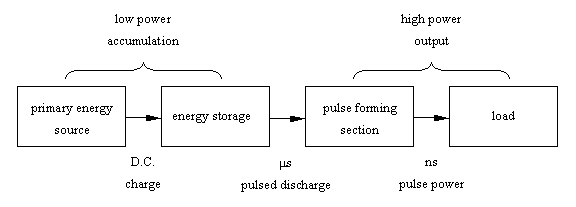
\includegraphics[height=4cm,width=8cm,keepaspectratio=true]{HPMsystem}
 \caption{Primjer ubacivanja slike.}
 \label{fig:prva}
	\end{center}
\end{figure}
\end{verbatim}
Uo�ite uporabu naredbe \verb|\label| unutar bloka. Na nju se potom u tekstu mo�emo referencirati pisanjem npr.\ \verb|Na Slici~\ref{fig:prva}| �ime \LaTeX{} u tekst uvrsti pripadaju�i broj slike, kao npr.\ ``Na Slici~\ref{fig:prva} prikazana je osnovna shema HPM sustava.''
Znak \verb|~| iza rije�i Slici osigurava to�no jedan znak razmaka, �to poma�e ukoliko je rije� Slika na kraju retka, da ne razdvoji rije� Slika i pripadaju�i broj slike.

\begin{figure}[!htbp]
	\begin{center}
 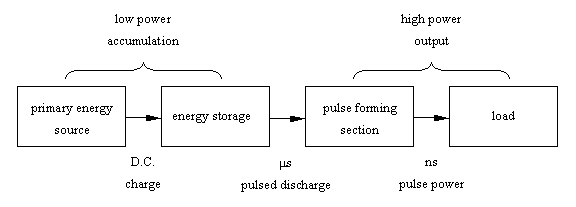
\includegraphics[height=4cm,width=8cm,keepaspectratio=true]{HPMsystem}
 \caption{Primjer ubacivanja slike.}
 \label{fig:prva}
	\end{center}
\end{figure}

Uo�ite i na�in prilago�avanja veli�ine slike. Parametri slike \emph{width} i \emph{height} odre�uju maksimalne dopu�tene dimenzije pri �emu se primarno po�tuje manju navedenu dimenziju, a \emph{keepaspectratio} osigurava zadr�avanje odnosa dimenzija slike, odnosno sprje�ava deformaciju slike, nakon proizvoljno unesenih veli�ina.

Uo�ite da sve oznake tj.\ \emph{labeli} ne smiju imati razmak u imenu. To vrijedi i op�enito, a ne samo za slike.

Tako�er, uo�ite da nije potrebno pisati ekstenziju slike jer to je ure�eno u postavkama glavnoga dokumenta pa time �tedi trud. Ekstenzije koje se mo�e izostaviti su: \emph{jpg}, \emph{jpeg}, \emph{png} i \emph{pdf}.

Shema prikazana na Slici~\ref{fig:prva} �e biti kori�tena i za potrebe idu�ih primjera, a {\color{blue} u mapi na va�em disku ju obri�ite nakon �to po�nete pohranjivati vlastite slike vezane uz va� rad}.


\section{Ubacivanje podslika}
Ponekada se jedna slika sastoji od dvije ili vi�e podslika kojima �elimo opisati neku cjelinu. Slika �e dobiti pripadni broj, a podslike slova (a), (b) itd.
To se mo�e posti�i sljede�om strukturom:
\begin{verbatim}
\begin{figure}[!htpb]
 \begin{center}
  \subfloat[Blok shema HPM sustava.]{\label{fig:HPM}
   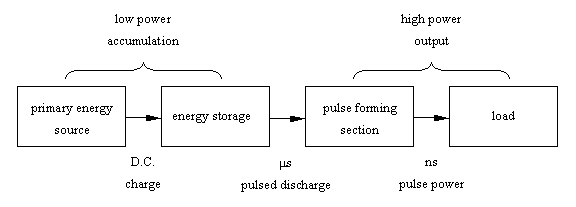
\includegraphics[height=5cm,width=10cm,keepaspectratio=true]{HPMsystem}}\\ 
	    %\hspace{10pt}
   \subfloat[JabRef su�elje za unos ``elektroni�ke'' reference.]
   {\label{fig:jabref}
   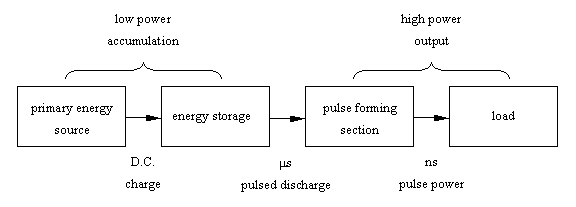
\includegraphics[height=7cm,keepaspectratio=true]{HPMsystem}}
\caption{Primjer ubacivanja vi�e podslika. Ovo je opis cijele slike.}
\label{fig:dvije_podslike}
  \end{center}
\end{figure}
\end{verbatim}
�to �e uvrstiti ono �to se vidi na Slici~\ref{fig:dvije_podslike}, koja se sastoji od dviju podslika.
Podslika~\ref{fig:HPM} pokazuje shemu HPM sustava, a podslika~\ref{fig:jabref} su�elje JabRef programa za unos bibliografskih jedinica.

\begin{figure}[!htpb]
	  \begin{center}
	   \subfloat[Blok shema HPM sustava.]{\label{fig:HPM} 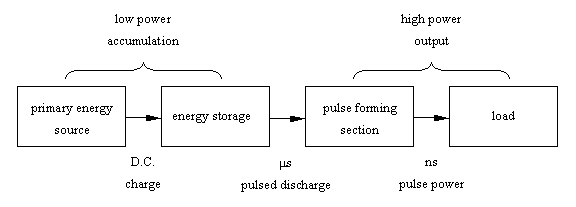
\includegraphics[height=5cm,width=10cm,keepaspectratio=true]{HPMsystem}} \\ %\hspace{10pt}
	   \subfloat[JabRef su�elje za unos ``elektroni�ke'' reference.]{\label{fig:jabref} 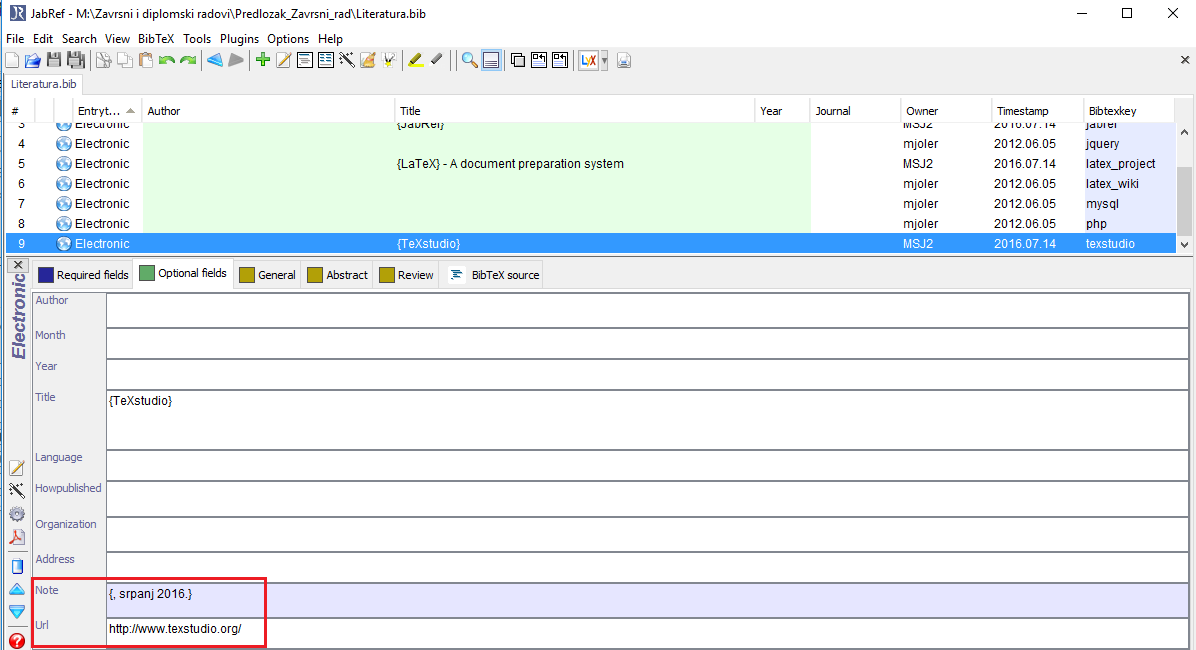
\includegraphics[height=7cm,keepaspectratio=true]{jabref}}
\caption{Primjer ubacivanja vi�e podslika. Ovo je opis cijele slike.}
\label{fig:dvije_podslike}
	  \end{center}
\end{figure}



\section{Ubacivanje tabele} 
Vi�e detalja o kreiranju tabela pro�itajte u literaturi, a sljede�i blok vam omogu�ava kreiranje jednostavne tabele, kao �to je prikazano u Tabeli~\ref{tab:prva}.
\begin{verbatim}
\begin{table}[!htbp]
\renewcommand{\arraystretch}{1.2}
\caption{Ovo je primjer izrade tabele.}
\centering
\begin{tabular}{|c|c|c|}
\hline
variabla & vrijednost 1 & vrijednost 2  \\ [0.5ex]
\hline \hline  
A & 5 & 3 \\ [0.5ex] % razmak do iducega retka
B & 4 & 2 \\ [0.5ex]
\hline
\end{tabular}
\label{tab:prva}
\end{table}
\end{verbatim}

\begin{table}[!htbp]
\renewcommand{\arraystretch}{1.2}
\caption{Ovo je primjer izrade tabele.}
\centering
\begin{tabular}{|c|c|c|}
\hline
variabla & vrijednost 1 & vrijednost 2  \\ [0.5ex]
\hline \hline 
A & 5 & 3 \\ [0.5ex] % razmak do iducega retka
B & 4 & 2 \\ [0.5ex]
\hline
\end{tabular}
\label{tab:prva}
\end{table}
%
Podaci koji su u stupcima se u tabeli razdvajaju znakom \&. Novi redak se na kraju aktualnoga retka formira znakom \verb|\\|. Broj stupaca se definira iza \emph{tabular} time �to se navedu slova koja ozna�avaju poravnavanje teksta u svakom stupcu, a broj slova zna�i broj stupaca koji �e biti kreiran u tabeli. Vertikalni razmak izme�u redaka u tabeli mo�ete za cijelu tabelu prilagoditi uporabom sljede�e sintakse prije strukture za tabelu:\\
\verb| \renewcommand{\arraystretch}{1.2} | gdje broj u zagradi na kraju (ovdje je 1.2) prilagodite sukladno va�oj preferenciji. Mo�e se prilagoditi i razmak za svaki pojedini redak (uo�ite \verb|[0.5ex]| na kraju redaka), ali to je manje od interesa jer tipi�no �elimo da svi retci imaju jednaki razmak jedni od drugih.

Sli�no mo�ete u�initi i za razmak izme�u stupaca tabele navo�enjem sljede�e sintakse prije bloka tabele:\\
\verb| \renewcommand{\tabcolsep}{0.3cm} |.



\section{Uporaba kratica u tekstu. Automatsko generiranje popisa kratica.}  \label{sec:kratice}
Listu kratica definirajte u datoteci \verb|Kratice.tex| (vidjeti predlo�ak unutar datoteke). U redovitom tekstu, kraticu  mo�ete ubaciti kori�tenjem naredbe \verb|\gls{ID_kratice}| gdje je \verb|ID_kraticE| identifikator kratice kako je definiran u datoteci \emph{Kratice.tex}. Pri prvoj uporabi naredbe \verb|\gls|, ispisat �e se najprije puni naziv pojma pa u zagradi kratica, a kod svake sljede�e uporabe, ispisat �e se samo kratica. Na primjer, kada (nakon prethodnog deklariranja u datoteci \verb|Kratice.tex|) upotrijebite \verb|\gls{gsm}| prvi puta, u tekstu �e se ispisati \gls{gsm}, a kada upotrijebite \verb|\gls{gsm}| drugi puta i dalje, u tekstu �e se ispisati samo \gls{gsm} (usporedi s definicijom kratice u datoteci \verb|Kratice.tex|). 
 
{\color{red} Listu kratica generirate sljede�im postupkom:} \label{generiranje_liste_kratica}
\begin{enumerate}
	\item Pokrenite kompilaciju cijeloga teksta jedanputa (to �e generirati neke datoteke koje su potrebne za daljnju obradu, specifi�no one s ekstenzijama .ist i .glo).
	\item Otvorite \emph{Command Prompt} aplikaciju na va�em ra�unalu i postavite se u radnu mapu gdje su vam datoteke za diplomski rad. 
	\item Potom pokrenite \emph{makeindex} rutinu (ona �e tipi�no biti ve� prisutna na va�em ra�unalu) upisuju�i sljede�u sintaksu: \\
	\verb|makeindex   -s myDoc.ist  -o myDoc.gls   myDoc.glo| \\
	gdje naziv datoteke \emph{myDoc} treba zamijeniti nazivom va�e glavne .tex datoteke, (npr. \verb|JMBAG_Ime_Prezime.tex|).
	\item Pokrenite \LaTeX{} jo� jednom ili dva puta, ako treba, dok se u uvodu pdf dokumenta ne pojavi lista kratica (pod naslovom \emph{Pojmovnik}).	
\end{enumerate}

Mo�da isprva zvu�i slo�eno, ali zapravo nije (bar ne uz ovako precizne upute!). Svaki puta kada dodate nove definicije kratica, potrebno je ponoviti ovaj postupak da bi se a�urirale odgovaraju�e datoteke i uredno prikazala potpuna lista u pdf-u (a i izbjegle poruke o pogre�kama tijekom kompajliranja teksta). 

Nije te�ko nakon �to prvi puta pro�ete ovaj postupak i omogu�ava vam u tekstu biti dosljedan u uporabi odre�ene kratice. Da izbjegnete �u�enje, va�no je jo� re�i da �e se ovim postupkom automatski stvoriti tek lista kratica koje ste u tekstu upotrijebili uporabom sintakse \verb|\gls|, a ne na temelju liste definicija koje ste naveli u datoteci \verb|Kratice.tex|. Zato, ako nijednom u tekstu ne upotrijebite sintaksu \verb|\gls|, ne�e biti ispisan ni popis kratica tj.\ \emph{Pojmovnik}. {\color{blue} Kako \LaTeX{} na kraju uvijek nagradi trud koji je ulo�en u savladavanje njegove sintakse, pogodnost ovakvoga automatskoga kreiranja Pojmovnika je i to �to uz svaki kraticu \LaTeX{} automatski ispi�e i brojeve stranica na kojima se doti�na kratica pojavljuje!} U elektroni�kom pdf dokumentu, brojevi stranica su ujedno i hiper-veze na te stranice pa se tako mo�e odmah sko�iti na stranicu gdje je pojedina kratica upotrijebljena.

Ukoliko vam se prethodno opisani postupak �ini preslo�enim, popis kratica mo�ete napraviti i ru�no, isto pomo�u datoteke Kratice.tex, u kojoj tako�er postoji kratki predlo�ak i za takav pristup. Za to je onda u osnovnoj datoteci \verb|JMBAG_Ima_Prezime.tex| potrebno deaktivirati liniju koda koja po�inje sa \verb|\printglossary|, a aktivirati blok koji po�inje sa \verb|\begin{glossary}| i zavr�ava sa \verb|end{glossary}|.



\section{Nagla�avanje teksta}
\subsection{Navodnici}
Za navodnike s lijeve strane fraze (otvaranje navodnika) koristi se 2x jednostruki navodnik koji se na tipkovnici nalazi lijevo od broja 1, a za navodnike s desne strane fraze (zatvaranje navodnika), koristi se 2x jednostruki navodnik koji se na tipkovnici nalazi na tipki \emph{�}, �to proizvede npr.\ ``abc''.

{\color{blue} Alternativno, u ovom paketu je pripremljena i naredba {\color{red} \verb|\navod{abc}|} gdje je \emph{abc} tekst koji se stavlja izme�u navodnika, tj.\ \navod{abc}.}

\subsection{Kosa i podebljana slova}
Nagla�avanje neke rije�i ili fraze pomo�u kosih (italic) slova mo�emo dobiti uporabom naredbe {\color{red} \verb|\emph{abc}|} ili pomo�u  {\color{red}\verb|\textit{abc}|} gdje je \emph{abc} neki tekst koji se �eli naglasiti.

\textbf{Podebljana slova} mo�emo posti�i uporabom naredbe {\color{red} \verb|\textbf{abc}|} gdje je \textit{abc} neki tekst koji �elimo podebljati.

\section{Verbatim: okru�enje za doslovni tekst}
Verbatim okru�enje omogu�ava ispis teksta u izvornom obliku, bez da ga \LaTeX{} tuma�i po svojiim sintakti�kim pravilima. To je pogodno kada se na stranicu  npr.\ �eli kopirati dio programskoga koda iz nekog jezika i kada �elimo zadr�ati sve izvorne znakove u nekoj frazi, bez da \LaTeX{} po�ne javljati pogre�ke kod kompajliranja, �to bi se moglo pojaviti kada se ne bi koristilo \emph{verbatim okru�enje}, po�to bi neke znakove interpretirao kao pogre�ke u sintaksi.

Postoji kra�i i du�i oblik verbatima. Kra�i slu�i za kra�u frazu od jedne ili par rije�i, a du�i za vi�e redaka.

\noindent Kra�i oblik verbatima ima sintaksu: \verb+\verb|neka fraza|+

\noindent Du�i oblik verbatima ima sintaksu:\\
\verb|\begin{verbatim}| \\
\verb|neki tekst| \\
\verb|\end{verbatim}| \\


\section{Kreiranje jedne jednad�be ili serije jednad�ba}

\subsection{Kreiranje jedne jednad�be}
Jednad�ba se napi�e u posebnom matemati�kom modu koji se kreira pomo�u bloka:
\begin{verbatim}
	\begin{equation}
		 A = B + C   \label{eq:prva}
	\end{equation}
\end{verbatim}
�to �e dati sljede�i izgled:
\begin{equation}
	 A = B + C   \label{eq:prva}
\end{equation}
Da bi se na nju referenciralo, na �eljenom mjestu u tekstu upi�emo \verb|\eqref{eq:prva}|, �ime �e se uvrstiti njezin pripadni (automatski generirani) broj, a za potpuniji smisao mo�emo npr.\ napisati \verb| Jednad�ba~\eqref{eq:prva}|, rezultat �ega je da �e u tekstu pisati Jednad�ba~\eqref{eq:prva}. 
Ako ju se ne �eli numerirati, onda se nakon rije�i \emph{begin} stavi zvjezdica, tj.\ \verb|begin*{equation}|.

\subsection{Kreiranje grupe jednad�ba}
Grupa jednad�ba se kreira uporabom \emph{subequations} sintakse. Na primjer, sljede�i blok �e definirati dvije podjednad�be u grupi, gdje �e svaka biti numerirana istim brojem, a razlikovati slovom iza broja.
\begin{verbatim}
	\begin{subequations}
		\begin{align}
		        A &= B + C  	\label{subeq:prva} \\
		        D &= F + G		\label{subeq:druga}
		\end{align}
	\label{subeq:obje}
	\end{subequations}
\end{verbatim}

To �e u izlaznom dokumentu rezultirati sljede�im izgledom:
\begin{subequations}
\begin{align}
        A &= B + C  	\label{subeq:prva} \\
        D &= F + G		\label{subeq:druga}
\end{align}
\label{subeq:obje}
\end{subequations}
U \eqref{subeq:prva} je prikazano dobivanje vrijednosti $A$, a u \eqref{subeq:druga} je prikazano dobivanje vrijednosti $D$. Jednad�ba~\eqref{subeq:obje} je \emph{�uveni studentov zakon}!



\section{Liste}
Liste su �este forme u tekstu kojima se na pregledni na�in nabrajaju neke stavke. Stavke obi�no navodimo ili s to�kama na po�etku, s brojevima ili sa slovima. U \LaTeX-u su upravo ta tri stila unaprijed definirana, a mogu�e su i slo�enije definicije stilova i kombinacije lista.

\subsection{Lista s to�kama}
Lista s to�kama se postigne blokom
\begin{verbatim}
\begin{itemize}
    \item prva nenumerirana stavka
    \item druga nenumerirana stavka
\end{itemize}
\end{verbatim}
�to na ekranu proizvede:
\begin{itemize}
% \setlength\itemsep{1ex}   % za lokalnu prilagodbu
	\item prva nenumerirana stavka
	\item druga nenumerirana stavka
\end{itemize}

\subsection{Lista s brojevima}
Numerirana lista s brojevima se postigne blokom
\begin{verbatim}
\begin{enumerate}[itemsep=1ex, topsep=4pt, partopsep=0pt]
     \item prva numerirana stavka
     \item druga numerirana stavka
\end{enumerate}
\end{verbatim}
U uglatoj zagradi su tri parametra kojima se to�no mo�e kontrolirati vertikalni razmak izme�u stavki u listi (\emph{itemsep}), razmak izme�u prethodnoga teksta i prve stavke u listi (\emph{topsep}) i dodatni prostor izme�u liste i prethodnoga paragrafa kada lista zapo�inje novi paragraf (\emph{partopsep}), ali te parametre \textbf{ne morate navoditi} tj.\ tu uglatu zagradu ne morate pisati. Tada �e se primijeniti vrijednosti parametara koje su definirane za cijeli dokument, a ove parametre se mo�e upotrijebiti tek da u nekom pojedinom slu�aju prilagodite razmake.
Za osjetiti efekte ovih parametara, najbolje se malo sam poigrati razli�itim vrijednostima parametara i vidjeti posljedice toga na listu (pri tome se uz brojeve kao prikladne jedinice za razmak mogu koristiti \emph{pt}, \emph{ex} ili \emph{em}).

\subsection{Proizvoljno ozna�ena lista}
Takva se lista mo�e posti�i u sklopu op�enitije forme koja omogu�uje proizvoljni opis ispred pojedine stavke, pomo�u sljede�ega bloka:
\begin{verbatim}
\begin{description}
     \item[a)] prva opisna stavka
     \item[b)] druga opisna stavka
\end{description}
\end{verbatim}
�to na ekranu proizvede:
\begin{description}%[itemsep=1ex, topsep=4pt, partopsep=0pt] za lokalnu prilagodbu
	\item[a)] prva opisna stavka
	\item[b)] druga opisna stavka \\
\end{description}
%
Kod ove strukture, u uglatu zagradu iza naredbe \verb|\item|, navodi se proizvoljna oznaka kojom se �eli na neki na�in ``numerirati'' listu.
%:::::::::::::::::::::::::::::::::::::::::::::::::::
\chapter{Dodatne informacije}
\section{Primjeri uporabe sintakti�kih struktura}
\begin{enumerate}
	\item Za uvid u kontekstualnu primjenu raznih sintakti�kih struktura, mo�ete otvoriti datoteku \href{run:Intro.tex}{{\color{blue}Intro.tex}}, unutar koje su napisane i ove upute. 
	\item Primjere slo�enijih sintakti�kih struktura, kao �to su ubacivanje slike, tabele ili jednad�be, mo�ete na�i u datoteci \href{run:sintaksa_cestih_struktura.tex}{{\color{blue}sintaksa\_cestih\_struktura.tex}} koja je dio paketa. Odabrane se strukture mo�e kopirati i zalijepiti u va� tekst, uz minimalne prilagodbe kao �to su naziv slike, veli�ina slike, opis i ID slike, a analogno i za tabele i jednad�be.
	\item Kona�no, za vi�e detalja o bilo �emu, potra�ite informacije u dvama priru�nicima koji su prilo�eni u mapi \href{run:prirucnici}{{\color{blue}prirucnici}} ili na webu, gdje se, me�u obiljem drugih informacija, nalaze i korisne wiki stranice \cite{latex_wiki,tex_exchange} o \LaTeX-u pomo�u kojih se obi�no brzo prona�e upute i zadovoljavaju�e rje�enje kakvom sintaksom se mo�e urediti �eljeni dio teksta.
\end{enumerate}

\section{Savjeti za lak�e ure�ivanje teksta}
Vjerujem da vam ovaj dokument mo�e uvelike pomo�i u pripremi teksta va�ega zavr�nog/diplomskog rada i omogu�iti da glavninu vremena tro�ite na sadr�aj rada, a manje na formatiranje rada jer to �e za vas sada obaviti \LaTeX{}! 

No, korektnosti radi, potrebno je napomenuti i sljede�e: \LaTeX{} je vrlo osjetljiv na pogre�ke u sintaksi naredbi (da, ba� kao �to su i programski jezici) pa vas mo�e povremeno ugnjaviti javljanjem pogre�ke koju nikako ne uspijevate uo�iti gdje je. Iskustvo kojim se izbjegava ta nelagoda jest sljede�e:
\begin{itemize}
	\item svako poglavlje napi�ite u novoj datoteci (da biste koli�inu teksta razdvojili na preglednije i manje cjeline) koju imenujte prikladnim imenom (bez razmaka u imenu). Potom te datoteke samo pozivajte iz glavnoga dokumenta \verb|JMBAG_Ime_Prezime.tex| pomo�u naredbe \verb|\include{ime_datoteke}|. Takav je pristup upravo i kori�ten u pripremi ovoga paketa.
	%
	\item {\color{red} budite koncentrirani dok pi�ete \LaTeX{} naredbe, poglavito zagrade, posebne znakove i matemati�ki tekst gdje se zahtijeva uporaba znaka \$!}
	%
	\item kompajlirajte tekst prije nego se skupi puno teksta jer tako �ete imati manje teksta za prekontrolirati u slu�aju pogre�ke. Tako�er vam za provjeru tek manjega dijela dokumenta mo�e pomo�i paket \verb|\usepackage{syntonly}| i naredba \verb|syntaxonly|, a isto tako i naredba \verb|\includeonly{ime_datoteke}| kojom �ete kompajlirati samo tu navedenu datoteku, �ime  ispred ``ne�eljenih'' datoteka ne morate stavljati znak ``komentara'' (\%).
	%
	\item ako niste sigurni ho�e li vam raditi neka naredba nakon pisanja, radije tekst kompajlirajte odmah po pisanju te naredbe---da vidite �to �ete dobiti i rije�ite dvojbu, nego da �ekate da se skupi jo� dubioznih mjesta u tekstu, kada �e nakon kompajliranja biti te�e detektirati koja linija teksta zapravo izaziva probleme (\LaTeX-ov prozor s porukama �esto nije odve� precizan u lociranju i opisu pogre�aka, ovisno o editoru teksta koji koristite).
\end{itemize}


\section{Zavr�ne napomene}
Ovime zaklju�ujemo uvodne upute koje �e najve�em broju studenata biti dovoljne (ili barem dovoljna osnova) za uspje�no pisanje zavr�nog odnosno diplomskog rada.

Prije nego prije�ete na kreiranje vlastitoga sadr�aja u�inite jo� sljede�e akcije kojima �ete deaktivirati dio paketa koji �e biti nepotreban:
\begin{enumerate}
	\item u mapi \href{run:slike}{{\color{blue}slike}}, obri�ite datoteke \verb|HPMsystem.png| i \verb|jabref.png| jer su one slu�ile tek za ilustracije u ovim Uputama.
	%
	\item u glavnoj datoteci  \href{run:JMBAG\_Ime\_Prezime.tex}{{\color{blue}JMBAG\_Ime\_Prezime.tex}} stavite znak komentara ``\%'' ispred linije \verb|\chapter{Kako koristiti paket za pisanje zavr�noga rada u \LaTeX-u}
Ovo su uvodne napomene za kori�tenje predlo�ka za pisanje zavr�noga ili diplomskoga rada studenata Tehni�koga fakulteta u Rijeci. Prije kori�tenja paketa, pro�itajte ovaj tekst jer �e vam dati nu�ne uvodne informacije, znatno vam olak�ati i ubrzati ure�ivanje teksta nakon toga, pri �emu �e vas i voditi kroz uporabu ovoga paketa na prakti�an na�in.

Paket je pripremljen tako da student �to prije mo�e pisati vlastiti tekst u ve� pripremljenom predlo�ku koji �e, uz minimalno u�enje sintakse \LaTeX-a, studentu olak�ati urediti svoj rad. U paketu su uklju�ene potrebne upute i sintakti�ke strukture koje bi trebale udovoljiti potrebama ve�ine studenta, a dodatne informacije postoje u dvama priru�nicima koji su uklju�eni u ovom paketu te, naravno, na raznim web stranicama na internetu koje su posve�ene \LaTeX-u (vidi u nastavku).

{\color{red} POZOR: paket treba biti prekopiran negdje na disk ne mijenjaju�i originalnu strukturu mapa (foldera) i ne mijenjaju�i nazive datoteka koje su u mapi \emph{tex\_aux}!}


\section{Opis sadr�aja paketa}
\vspace{-2ex}
Paket se sastoji od:
\begin{itemize}
 \item datoteke \href{run:UPUTE.pdf}{{\color{blue} UPUTE.pdf}} koja sadr�i postupak instalacije potrebnih alata na ra�unalo te kori�tenja paketa. \emph{UPUTE} su bazirane na Windows OS, a korisnici drugih OS-ova si na nazna�enim web lokacijama samo trebaju na�i instalacije za njihov OS.
 %
 \item datoteke \verb|JMBAG_Ime_Prezime.tex| koja je sredi�nja datoteka koja povezuje sve cjeline i kompajliranjem koje se dobije izlazni \verb|JMBAG_Ime_Prezime.pdf| dokument (naravno, tijekom rada, upisat �ete svoj specifi�ni JMBAG i ime i prezime).\\ U ovoj se datoteci inicijalno nalaze i upute za kori�tenje paketa kao i primjeri osnovne uporabe naj�e��ih sintakti�kih struktura u \LaTeX-u koje bi trebale biti dovoljne ve�ini studenata za pisanje rada.
 %
 \item mape \verb|tex_aux| u kojoj su \emph{interne datoteke} koje definiraju stilove, formate i sl.\ koji slu�e u slaganju izlaznoga formata. \textbf{Student/ica s njima ne treba \emph{ni�ta} raditi}, ali one trebaju biti u \verb|tex_aux| mapi pod glavnom mapom zavr�noga rada, kao �to je postavljeno u ovom paketu.
 %
 \item mape \emph{slike} u koju student treba pohraniti sve slike koje �e koristiti u radu. Ime mape se ne smije preimenovati bez boljega poznavanja sintakse \LaTeX-a jer ovaj paket da bi ispravno radio o�ekuje ba� takvo ime mape!
 %
 \item datoteke \verb|sintaksa_cestih_struktura.tex| koja ne sudjeluje izravno u kompajliranju pdf dokumenta, nego slu�i kao repozitorij u kojemu su sadr�ane naj�e��e potrebne sintakti�ke strukture koje su spremne za kopiranje u va� tekst uz minimalnu prilagodbu parametara (npr.\ opis slike, ime datoteke specifi�ne slike koju se ubacuje i proizvoljni ID te slike za kasnije referenciranje).
 %
 \item mape \href{run:prirucnici}{{\color{blue}prirucnici}} u kojoj se nalazi nekoliko najpopularnijih priru�nika za uporabu \LaTeX-a. 
\end{itemize}
%%%%%%%%%%%%%%%%%%%%%%%%%%%%%%%%%%%%%%%%%%%%%%%%%%%%%%%%%%%%%%%

\section{�ime se opremiti za pisanje rada}
Da bi se rad napisao pomo�u \LaTeX-a (a to vrijedi svake lipe!), najprije je na ra�unalo potrebno instalirati:
\begin{enumerate}
	\item obavezno: \LaTeX{} software 
	\item obavezno: editor za ure�ivanje teksta 
	\item neobavezno, ali korisno: softver za opis literature. (Premda dodatni softver nije nu�an jer se popis literature mo�e obraditi i ru�no (no to je manje sofisticirano kod uvr�tavanja referenca), sugeriram instalaciju softvera koji pomo�u intuitivnih su�elja korisniku omogu�ava opis pojedine kori�tene literature (kao mala baza podataka), a potom se pojedina jedinica literature jednostavno ubacuje u tekst, a popis literature se na kraju automatski formira (vi�e o tome pro�itajte u nastavku).
\end{enumerate}

\subsection{Instalacija \LaTeX-a}
\begin{enumerate}
	\item odite na sredi�nji \LaTeX{} portal \cite{latex_project}: \url{http://www.latex-project.org/}
	\item kliknite na poveznicu \href{http://www.latex-project.org/ftp.html}{Getting LaTeX} i potom uo�ite i povucite instalaciju koja odgovara va�em OS-u (npr.\ proTeXt za Windows, MacTeX za Mac, TeX Live za Linux). Pozor: instalacijski paket je velik i mo�e du�e potrajati �ak i na brzoj vezi---dajte si dovoljno vremena za obaviti download.
	\item Instalirajte \LaTeX{} slijede�i upute koje su prilo�ene za odabranu instalaciju (npr.\ proTeXt za Windowse daje kratki pdf s uputama koje vas vode kroz instalaciju korak po korak).
\end{enumerate}

\subsection{Instalacija editora teksta}
Instalirajte editor koji je pogodan za pisanje \LaTeX{} koda. \textbf{Za Windows OS, toplo preporu�am}  \href{http://www.texstudio.org}{{\color{blue} TeXstudio}} \cite{texstudio} jer je bogat opcijama, ugodan za rad i stabilan, a instalacije postoje i za Linux i Mac OS. TeXstudio se zasebno povu�e i instalira na ra�unalo, a neke editore teksta koji ve� do�u u paketu za instalaciju LaTeXa mo�ete ignorirati (npr.\ za Windows je do nedavno bio popularan \emph{TeXnicCenter} i dolazi ve� upakiran u proTeXt-u (a mo�da �ete na�i i \emph{TeXworks}), za Mac je kvalitetan \emph{TeXShop} koji sada tako�er dolazi u paketu s MacTeX-om). 

\label{encoding1} {\color{red} POZOR: Premda �e ovo biti jo� napomenuto na stranici~\pageref{encoding2}, prije samoga po�etka pisanja va�ega rada, �to prije �elim napomenuti sljede�i va�ni detalj: za svaki va� tekst koji pi�ete u editoru teksta, uvjerite se da je kodna stranica postavljena na \navod{windows-1250}, �to je klju�no da bi se u izlaznom pdf-u ispravno ispisivali hrvatski dijakriti�ki znakovi! U TeXstudiu, aktualnu kodnu stranicu se mo�e vidjeti i promijeniti preko maloga izbornika u doljnjem desnom kutu glavnoga prozora, gdje se nalazi opcija ``Encoding''. Ukoliko tu ne pi�e ``windows-1250'', kliknite na izbornik, odaberite opciju ``More Encodings'' pa u potom otvorenom su�elju odaberite kodnu stranicu ``windows-1250 / CP 1250'' i potvrdu sa ``Change To''.}

\subsection{Instalacija programa za opis kori�tene literature}
\emph{Ponavljamo: Kori�tenje BiBTeX programa za opis literature \textbf{nije} neophodno, ali jest korisno. U datoteci po imenu \href{run:Literatura.tex}{{\color{blue}Literatura.tex}}, koja je uklju�ena u ovaj paket, ve� su namje�tene postavke kao da �e se literatura opisati pomo�u BiBTeX programa (npr.\ JabRef-a) i ne treba ni�ta mijenjati, ali ispod toga se mo�e prona�i i upute i za drugi--ru�ni-- na�in (p)opisivanja literature.}

Kao bibtex program za opis literature, preporu�am \href{http://www.jabref.org}{{\color{blue} JabRef}} program \cite{jabref}. To je legalno besplatno dostupni program za Windows OS (ali postoji i za Mac, a i platformski neovisna instalacija) koji nam omogu�ava opisivanje literature na lak na�in pomo�u intuitivnih su�elja, a kao rezultat kreira \emph{BibTeX} datoteku \emph{Literatura.bib} (gdje je (\emph{Literatura} naziv koji korisnik treba dodijeliti pri pohrani JabRef datoteke na disk u slu�aju ovoga predlo�ka, da bi paket funkcionirao) u kojoj je literatura opisana na na�in koji \LaTeX{} razumije. 

Uo�ite da ako ne koristite JabRef, ve� se odlu�ite za ru�ni unos literature, �to se isprva doima jednostavnijim, tada �e vam redoslijed referenca u popisu literature odgovarati to�no redoslijedu koji ste naveli u tom popisu --- dakle morate paziti da redoslijed formirate onim redom kojim pozivate reference u va�em tekstu (�to kod nekog kasnije ubacivanja dodatne reference unutar ve� postoje�ega redoslijeda tra�i brigu da ju se ubaci na odgovaraju�e mjesto u popisu literature), a tako�er trebate paziti i na formatiranje teksta svake reference! 

Za razliku od toga, kori�tenjem JabRef-a, izbjegavate ru�no formiranje popisa literature i ne trebate brinuti o redoslijedu referenca, ve� samo pomo�u JabRefa trebate unijeti sve jedinice literature koju �ete navesti, a \LaTeX{} �e vam automatski formirati listu referenca onim redoslijedom kojim reference bude pozivali u tekstu!

Nakon �to kompajlirate projekt, stvorit �e vam se pomo�na datoteka imena \href{run:JMBAG_Ime_Prezime.bbl}{{\color{blue}JMBAG\_Ime\_Prezime.bbl}} u kojoj �e jedinice literature tijekom kompilacije biti formatirane i odatle se ubacuju u kona�nu verziju teksta. Stoga, \textbf{ukoliko ima ikakvih detalja koje u opisu literature treba prilagoditi, a ne mo�ete automatskim putem}, uvijek vam kao ``zadnja crta obrane'' ostaje otvoriti \verb|bbl| datoteku i tamo ru�no napraviti izmjene. Potom ponovo kompajlirajte projekt i te �e se promjene vidjeti u pdf-u tj.\ ru�no unijete promjene ne�e biti poni�tene sve dok ne obri�ete cijelu datoteku.

Umjesto da rukom pi�ete cijelu bibliografiju, vremenski vam je vjerojatno u�inko\-vitije popis literature generirate uporabom JabRef-a, a potom ako i�ta jo� treba prilagoditi, onda samo to napraviti ru�no u \verb|bbl| datoteci.


\subsubsection{Osnovna uporaba JabRef programa}
Upoznajte se s najva�nijim opcijama u \emph{JabRef}-u:
\begin{itemize}
	\item uo�ite ikonu (pod znakom ``+'' i tekstom \emph{New BibTeX Entry}) za unos nove jedinice literature (npr. knjige, �lanka, web portala i sl.)
	%
	\item kada kliknete za unos nove stavke literature, uo�ite kakvi se sve tipovi literature nude za odabir. Odabirom opcije koja odgovara naslovu koji �elite unijeti, otvorit �e vam se novi prozor s poljima u koja se mo�e unijeti informacije o literaturi. Za odabrani tip literature samo su neka polja obavezna (nalaze se pod karticom (eng.\ \emph{tabom}) \emph{Required fields}), dok se pod drugim karticama mo�e i ne mora unijeti dodatne informacije. U slu�aju na�ih zavr�nih/diplomskih radova, bit �e znatan udjeli literature koja je na internetu pa za formatiranje iste, pro�itajte upute i napomene u nastavku ove sekcije.
	%
	\item kada je vi�e autora, njihova imena se u JabRefu polju za unos autora razdvajaju pisanjem klju�ne rije�i \verb|and| (a ne razmakom, zarezom ili to�ka-zarezom!)
	%
	\item U popisu literature se ne�e uvijek pojam prepisati onako kako ste ga vi zapisali u JabRefu! To je posljedica stilova koji su definirani u \verb|bst| datoteci (ne zamarajte se time sada jer je za naprednu razinu \LaTeX-a). No, ako neki pojam ba� ne ispadne suvislo napisan u popisu literature ili ba� �elite forsirati odre�eni na�in zapisa (�esto slu�aj kada se rije� s velikim slovima ne interpretira onako kako �elite), tada to�no odre�eni zapis mo�ete forsirati na na�in da \verb|{tu rije� ili frazu stavite unutar viti�astih zagrada}|
	%
	\item prije nego pohranite pojedinu stavku pomo�u \emph{Ctrl+S}, \textbf{morate svakoj jedinici literature dodijeliti jedinstveni identifikator}, tzv.\ \emph{Bibtexkey}, �to je jedno od polja koja su obavezna za unos. Mo�ete ru�no upisati neki proizvoljni string, ali pogodnije je generirati ga automatski.\\ Za to u�initi me�u ikonama na vrhu imate ikonu koja izgleda kao (�arobni) �tapi� sa zvjezdicama oko njega, klikom na kojega \emph{JabRef} automatski dodijeli jedinstveni BibTeX \emph{klju�} za tu bibliografsku jedinicu. Pomo�u toga klju�a se poslije bilo kada i bilo gdje u pisanju va�ega rada mo�ete pozvati na tu referencu, a \LaTeX{} �e sve ostalo obaviti za vas tj.\ dodijeliti joj odgovaraju�i broj u tekstu i s tim brojem uvrstiti u popis literature.
	%
	\item korisnik ima mogu�nost i promijeniti uzorak po kojem se kreira struktura automatski generiranoga jedinstvenoga BibTeX klju�a tako da se otvori opcija izbornika \emph{Options $>>$ Preferences $>>$ BibTeX key generator}, gdje je na vrhu prozora prikazan \emph{default} uzorak, npr. \verb|[auth]:[year]| �to zna�i da se klju� kreira na bazi \verb|prezime(autora):godina(rada)|. To se sada mo�e urediti po nekom novom uzorku, no ovako definirani uzorak u biti zadovoljava, a ako igdje ima potrebe za dodatnim razlikovanjem, mo�e se na automatski generiranom klju�u jo� ru�no napraviti korekcija dodavanjem nekog znaka na kraju, kao npr.\ dodavanjem \verb|_a| i sl. (Klikom na karticu \emph{BibTeX source} mo�ete vidjeti kako �e unos va�ih podataka zapravo biti zapisan u va�oj \emph{Literatura.bib} datoteci koja �e se formirati od svih bibliografskih jedinica koje unesete.)
	%
	%
	\item Za \emph{ime} va�e bibliografske datoteke kod pohrane na disk obavezno upi�ite  \emph{Literatura} jer to ime o�ekuje ovaj paket. Pozor: Datoteka \emph{Literatura.bib}, koju ste tako kreirali, mora se nalaziti unutar mape ovoga paketa da bi sve ispravno radilo! U paketu je za primjer ve� kreirana jedna datoteka istoga imena koju za vje�bu student mo�e i otvoriti u \emph{JabRef}-u, ali to su samo pokazne bibliografske jedinice unesene kao primjer, koje student treba u kona�nici zamijeniti svojim bibliografskim jedinicama.
	%
	\item Za ``elektroni�ke'' izvore literature (tj.\ sve �to ste kao informaciju na�li na webu), JabRef nudi tip literature pod nazivom ``Electronic'' (vidi Sl.~\ref{fig:jabref}). U njemu pod karticom (eng.\ tabom) \emph{Optional fields} pod poljem \verb|Title| mo�ete upisati ime web stranice (autor, tvrtka i sl.), pod poljem \verb|url| mo�ete upisati URL adresu te web stranice, a pod poljem \verb|Note| upisati datum kada ste posjetili tu web stranicu (npr.\ \emph{srpanj 2016.} ili \emph{3.~rujna~2016.}). Rezultat toga �e u pdf-u biti da je sve napisano redoslijedom koji je predvi�en u Uputama RiTeha za pisanje diplomskog rada \cite{riteh_upute}, \emph{osim �to u ovom Predlo�ku do sada nisam uspio rije�iti ubacivanje zareza izme�u URL adrese i datuma posjeta toj URL adresi}, koji bi ta dva podatka odvojio, pa je tu potrebna mala ru�na \emph{prilagodba na jedan od ovih dvaju na�ina}:
	\begin{enumerate}[label=\textbf{\roman*)}]
		\item kod unosa datuma u polje \verb|Note| (u su�elju JabRef-a), upi�ite datum na sljede�i na�in: \verb|{, <datum>}|, gdje je \verb|<datum>| va� specifi�ni datum, dok �e \emph{zarez} iza prve zagrade izvr�iti razdvajanje URL adrese i datuma, a \textbf{viti�aste zagrade} osigurati da se to ba� tako to�no prenese u pdf-dokument (uklju�uju�i i da se mjesec napi�e malim po�etnim slovom, �to ina�e ne bi bio slu�aj). (Za neke druge tipove referenca kao npr.\ tip \emph{manual}, zarez vam prije datuma ne�e trebati jer �e naziv literature zavr�iti zarezom.) U Jabrefu vam i ina�e vrijedi da kada �elite forsirati da se pojam ba� to�no u popisu literature zapi�e onako kao ste htjeli, onda se pojam stavi unutar viti�astih zagrada \verb|{kao u ovom primjeru}|.
		\item ako u polju \verb|Note| ne upi�ete datum na prethodno opisani na�in, onda vam u pdf dokumentu ne�e biti upisan zarez izme�u URL adrese i datuma koji ste unijeli, a tako�er �e i mjesec biti napisan velikim po�etnim slovom (�to nije stra�no, ali je manje po�eljno). To mo�ete \emph{ru�no} prilagoditi tako da otvorite \verb|.bbl| datoteku i pomo�u \emph{Find/Replace} operacije sve nazive mjeseca zamijenite na na�in da po�inju malim po�etnim slovom (�to nije te�ko kada vam je ve�ina datuma u popisu literature navedena u istom mjesecu), ali zareze �ete svakako morati ubacivati ru�no u svaku pojedinu stavku literature jer ne�e biti nekog predlo�ka kojim biste to rije�ili automatski pomo�u \emph{Find/Replace} operacije. Na kraju opet kompajlirajte projekt. S obzirom na navedeno, prvi na�in je vremenski �tedljiviji!
	\end{enumerate}
\end{itemize}

%%%%%%%%%%%%%%%%%%%%%%%%%%%%%%%%%%%%%%%%%%%%%%%%%%%


\chapter{Primjeri naj�e��ih sintakti�kih struktura}
Prije stvarnoga po�etka pisanja svoga rada, upoznajte se s osnovnim sintakti�kim strukturama koje �e vam trebati tijekom pisanja rada.

U nastavku su opisane naj�e��e sintakti�ke strukture (dio njih mo�ete na�i i u datoteci \emph{Intro.tex}), a dodatne slo�enije strukture su pohranjene u datoteci \href{run:sintaksa_cestih_struktura.tex}{{\color{blue}sintaksa\_cestih\_struktura.tex}} koja je sastavni dio glave mape ovoga paketa. 

\section{Postavljanje naslova poglavlja i sekcija}
\begin{itemize}
	\item \verb|\chapter{Naslov poglavlja}|: za definiranje naslova poglavlja
	\item \verb|\section{Naslov sekcije}|: za definiranje naslova sekcije unutar poglavlja
	\item \verb|\subsection{Naslov podsekcije}|: za definiranje naslova podsekcije
\end{itemize}


\section{Reference na literaturu} \label{sec:RefLit}
Za referencu na pojedini kori�teni izvor informacije (tj.\ jedinicu literature), koristimo naredbu \\
\verb|\cite{bibtexkey}|, gdje je \emph{bibtexkey} jedinstveni klju� kojim prethodno ozna�imo tu jedinicu literature. \verb|Bibtexkey| mo�emo definirati na jedan od sljede�ih na�ina:
\begin{description}
	\item[I)] ako popis literature definiramo izravno u datoteci \href{run:Literatura.tex}{{\color{blue}Literatura.tex}} (opcija (I) u datoteci), onda ispred svake stavke literature treba definirati i jedinstveni \verb|bibtexkey| pomo�u naredbe \verb|\bibitem{bibtexkey}| (vidi predlo�ak u datoteci)
	\item[II)] ako literaturu opisujemo pomo�u JabRef datoteke \emph{Literatura.bib} (opcija (II) u datoteci), onda se tamo uz svaku stavku definira \verb|bibtexkey| (bude na dnu JabRef obrasca za upis pojedine jedinice literature)
\end{description}
%
Npr.\ ako negdje u tekstu napi�emo \verb|\cite{latex_wiki}|, gdje je \verb|latex_wiki| prethodno definirani \emph{bibtexkey}, tada �e se u tekstu u uglatoj zagradi pokazati broj  te bibliografske jedinice pod kojim se nalazi u popisu literature (Bibliografiji) na kraju rada (u ovom primjeru, to je broj \cite{latex_wiki}).


\section{Referenca na sekciju, sliku, tabelu ili stranicu} \label{sec:RefText}

Za referenciranje na pojedine dijelove teksta unutar rada, koristimo
{\color{red} \verb|\label{ID}|} i {\color{red} \verb|\ref{ID}|} na na�in da se \verb|\label{ID}| postavi uz dio teksta koji �elimo ozna�iti internom oznakom i poslije �emo se u tekstu na to referencirati, a \verb|\ref{ID}| upotrijebimo na mjestu s kojega se referenciramo na dio teksta koji je ranije ozna�en pomo�u \verb|\label{ID}|.

Ako se �elimo referencirati na specifi�nu sliku ili tabelu ili sekciju ili jednad�bu u tekstu, tada unutar bloka toga sadr�aja stavimo oznaku \verb|\label{prefiks:ID_objekta}| gdje je \emph{objekt} slika ili tablica ili sekcija teksta ili jednad�ba, a na �eljenom mjestu u tekstu se na to referiramo pomo�u \verb|\ref{prefiks:ID_objekta}| (u slu�aju referenciranja jednad�be, bolji oblik naredbe je {\color{red} \verb|\eqref{prefiks:ID_objekta}|}).

\verb|ID_objekta| je proizvoljni string (bez razmaka) koji dodijelimo objektu od interesa, a radi preglednijega ure�ivanja teksta, uobi�ajeno je u \LaTeX-u za pojedine tipove oznaka staviti i odgovaraju�i \emph{prefiks}, kao npr.\ \emph{sec} za oznaku sekcije, \emph{fig} za oznaku slike, \emph{tab} za oznaku tabele, \emph{eq} za oznaku jednad�be i sl. (Tako bi za sliku kojoj dodijelimo $ID=prva$ bilo \verb|\label{fig:prva}|, za tablicu \verb|\label{tab:prva}|, za sekciju \verb|\label{sec:prva}|, a za jednad�bu \verb|\label{eq:prva}|.)

Za referencirati se na \emph{stranicu} u tekstu gdje se nalazi ne�to na �to se �elite osvrnuti, koristi naredba {\color{red} \verb|\pageref{prefiks:ID_objekta}|}. Za njenu primjenu se tako�er prethodno treba ozna�iti �eljeni tekst pomo�u naredbe \verb|\label|.

Tako npr.\ mo�emo staviti da je primjer kreiranja tabele \emph{prva} opisan na stranici~\verb|\pageref{tab:prva}|, �to �e za rezultat imati tekst u kojem pi�e ``da je primjer kreiranja tabele \emph{prva} opisan na stranici~\pageref{tab:prva}'' (jer se u tekstu ta tabela nakon kompajliranja npr.\ na�e na stranici 12). Kako god se tekst smanjivao ili pove�avao i navedena tablica mijenjala broj stranice na kojoj se u kona�nici nalazi, mi ne moramo o tome brinuti jer \LaTeX{} brine o tome i na kraju napi�e to�ni broj stranice! (To je jo� jedna o pogodnosti zbog �ega se ljudi i odlu�e, uz ne�to po�etnoga truda, za kori�tenje \LaTeX-a!).



\section{Poveznica na neki dokument ili URL adresu}
Naredbe \verb|\url| i \verb|\href| slu�e za kreiranje poveznice na neku URL adresu ili neki dokument na disku.

{\color{red}\verb|\url{adresa}|} �e otisnuti URL adresu to�no onako kako je \emph{adresa} navedena unutar zagrada.

{\color{red}\verb|\href{akcija:destinacija}{opis}|} �e na papiru/ekranu ispisati tekst \emph{opis} koji je naveden u drugoj zagradi, i izvr�iti \emph{akciju} prema \emph{destinaciji} koja je navedena u prvoj zagradi. 
\emph{Akcija} mo�e npr.\ glasiti \emph{run} ili \emph{mailto}, gdje �e prvi oblik otvoriti mapu ili datoteku staza koje je navedena kao \emph{destinacija}, a drugi oblik pokrenuti pisanje emaila prema email adresi koja je navedena kao \emph{destinacija}.

Ne pretjerujte ipak s uporabom ovih struktura, odnosno uop�e ne morate to koristiti u radu, nego za vanjske reference koristiti samo \verb|\cite{bibtexkey}| naredbu, a za unutra�nje reference (na dijelove teksta) kombinaciju naredbi \verb|\label{ID}| i \verb|\ref{ID}| kako je to opisano u Sekciji~\ref{sec:RefText}. 


\section{Ubacivanje slike}
Sliku mo�emo ubaciti pomo�u sljede�ega bloka naredbi:
\begin{verbatim}
\begin{figure}[!htbp]
	\begin{center}
 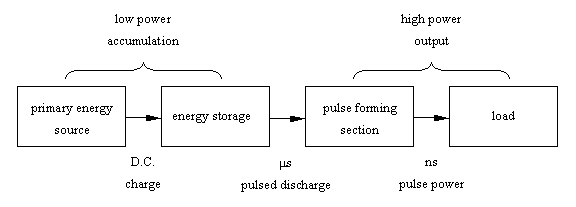
\includegraphics[height=4cm,width=8cm,keepaspectratio=true]{HPMsystem}
 \caption{Primjer ubacivanja slike.}
 \label{fig:prva}
	\end{center}
\end{figure}
\end{verbatim}
Uo�ite uporabu naredbe \verb|\label| unutar bloka. Na nju se potom u tekstu mo�emo referencirati pisanjem npr.\ \verb|Na Slici~\ref{fig:prva}| �ime \LaTeX{} u tekst uvrsti pripadaju�i broj slike, kao npr.\ ``Na Slici~\ref{fig:prva} prikazana je osnovna shema HPM sustava.''
Znak \verb|~| iza rije�i Slici osigurava to�no jedan znak razmaka, �to poma�e ukoliko je rije� Slika na kraju retka, da ne razdvoji rije� Slika i pripadaju�i broj slike.

\begin{figure}[!htbp]
	\begin{center}
 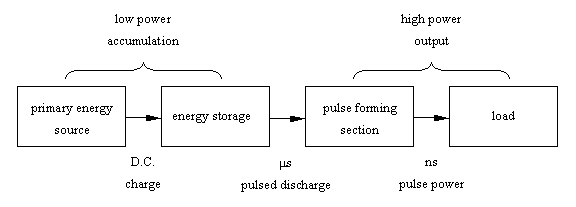
\includegraphics[height=4cm,width=8cm,keepaspectratio=true]{HPMsystem}
 \caption{Primjer ubacivanja slike.}
 \label{fig:prva}
	\end{center}
\end{figure}

Uo�ite i na�in prilago�avanja veli�ine slike. Parametri slike \emph{width} i \emph{height} odre�uju maksimalne dopu�tene dimenzije pri �emu se primarno po�tuje manju navedenu dimenziju, a \emph{keepaspectratio} osigurava zadr�avanje odnosa dimenzija slike, odnosno sprje�ava deformaciju slike, nakon proizvoljno unesenih veli�ina.

Uo�ite da sve oznake tj.\ \emph{labeli} ne smiju imati razmak u imenu. To vrijedi i op�enito, a ne samo za slike.

Tako�er, uo�ite da nije potrebno pisati ekstenziju slike jer to je ure�eno u postavkama glavnoga dokumenta pa time �tedi trud. Ekstenzije koje se mo�e izostaviti su: \emph{jpg}, \emph{jpeg}, \emph{png} i \emph{pdf}.

Shema prikazana na Slici~\ref{fig:prva} �e biti kori�tena i za potrebe idu�ih primjera, a {\color{blue} u mapi na va�em disku ju obri�ite nakon �to po�nete pohranjivati vlastite slike vezane uz va� rad}.


\section{Ubacivanje podslika}
Ponekada se jedna slika sastoji od dvije ili vi�e podslika kojima �elimo opisati neku cjelinu. Slika �e dobiti pripadni broj, a podslike slova (a), (b) itd.
To se mo�e posti�i sljede�om strukturom:
\begin{verbatim}
\begin{figure}[!htpb]
 \begin{center}
  \subfloat[Blok shema HPM sustava.]{\label{fig:HPM}
   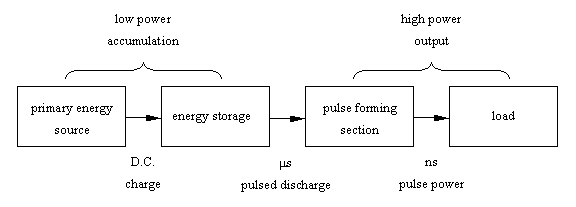
\includegraphics[height=5cm,width=10cm,keepaspectratio=true]{HPMsystem}}\\ 
	    %\hspace{10pt}
   \subfloat[JabRef su�elje za unos ``elektroni�ke'' reference.]
   {\label{fig:jabref}
   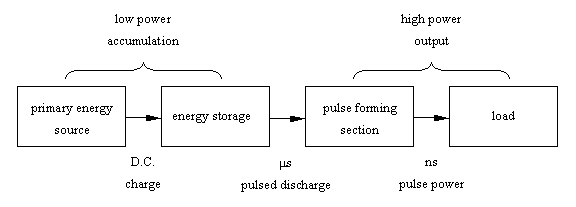
\includegraphics[height=7cm,keepaspectratio=true]{HPMsystem}}
\caption{Primjer ubacivanja vi�e podslika. Ovo je opis cijele slike.}
\label{fig:dvije_podslike}
  \end{center}
\end{figure}
\end{verbatim}
�to �e uvrstiti ono �to se vidi na Slici~\ref{fig:dvije_podslike}, koja se sastoji od dviju podslika.
Podslika~\ref{fig:HPM} pokazuje shemu HPM sustava, a podslika~\ref{fig:jabref} su�elje JabRef programa za unos bibliografskih jedinica.

\begin{figure}[!htpb]
	  \begin{center}
	   \subfloat[Blok shema HPM sustava.]{\label{fig:HPM} 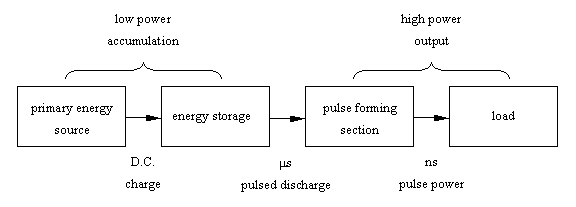
\includegraphics[height=5cm,width=10cm,keepaspectratio=true]{HPMsystem}} \\ %\hspace{10pt}
	   \subfloat[JabRef su�elje za unos ``elektroni�ke'' reference.]{\label{fig:jabref} 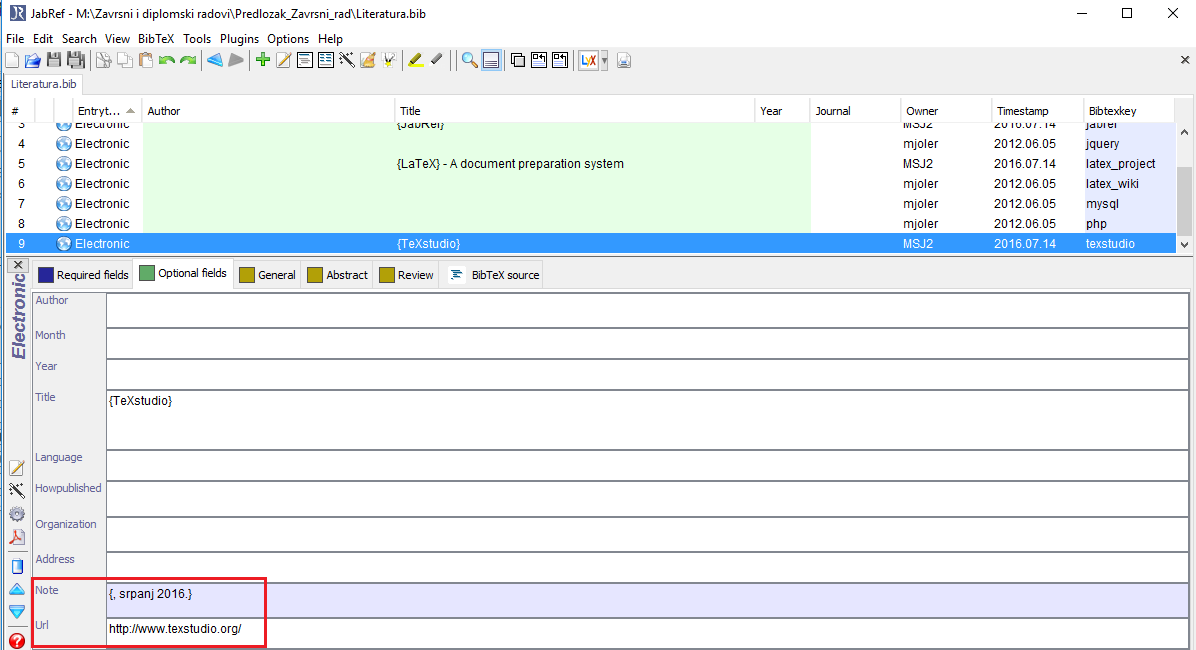
\includegraphics[height=7cm,keepaspectratio=true]{jabref}}
\caption{Primjer ubacivanja vi�e podslika. Ovo je opis cijele slike.}
\label{fig:dvije_podslike}
	  \end{center}
\end{figure}



\section{Ubacivanje tabele} 
Vi�e detalja o kreiranju tabela pro�itajte u literaturi, a sljede�i blok vam omogu�ava kreiranje jednostavne tabele, kao �to je prikazano u Tabeli~\ref{tab:prva}.
\begin{verbatim}
\begin{table}[!htbp]
\renewcommand{\arraystretch}{1.2}
\caption{Ovo je primjer izrade tabele.}
\centering
\begin{tabular}{|c|c|c|}
\hline
variabla & vrijednost 1 & vrijednost 2  \\ [0.5ex]
\hline \hline  
A & 5 & 3 \\ [0.5ex] % razmak do iducega retka
B & 4 & 2 \\ [0.5ex]
\hline
\end{tabular}
\label{tab:prva}
\end{table}
\end{verbatim}

\begin{table}[!htbp]
\renewcommand{\arraystretch}{1.2}
\caption{Ovo je primjer izrade tabele.}
\centering
\begin{tabular}{|c|c|c|}
\hline
variabla & vrijednost 1 & vrijednost 2  \\ [0.5ex]
\hline \hline 
A & 5 & 3 \\ [0.5ex] % razmak do iducega retka
B & 4 & 2 \\ [0.5ex]
\hline
\end{tabular}
\label{tab:prva}
\end{table}
%
Podaci koji su u stupcima se u tabeli razdvajaju znakom \&. Novi redak se na kraju aktualnoga retka formira znakom \verb|\\|. Broj stupaca se definira iza \emph{tabular} time �to se navedu slova koja ozna�avaju poravnavanje teksta u svakom stupcu, a broj slova zna�i broj stupaca koji �e biti kreiran u tabeli. Vertikalni razmak izme�u redaka u tabeli mo�ete za cijelu tabelu prilagoditi uporabom sljede�e sintakse prije strukture za tabelu:\\
\verb| \renewcommand{\arraystretch}{1.2} | gdje broj u zagradi na kraju (ovdje je 1.2) prilagodite sukladno va�oj preferenciji. Mo�e se prilagoditi i razmak za svaki pojedini redak (uo�ite \verb|[0.5ex]| na kraju redaka), ali to je manje od interesa jer tipi�no �elimo da svi retci imaju jednaki razmak jedni od drugih.

Sli�no mo�ete u�initi i za razmak izme�u stupaca tabele navo�enjem sljede�e sintakse prije bloka tabele:\\
\verb| \renewcommand{\tabcolsep}{0.3cm} |.



\section{Uporaba kratica u tekstu. Automatsko generiranje popisa kratica.}  \label{sec:kratice}
Listu kratica definirajte u datoteci \verb|Kratice.tex| (vidjeti predlo�ak unutar datoteke). U redovitom tekstu, kraticu  mo�ete ubaciti kori�tenjem naredbe \verb|\gls{ID_kratice}| gdje je \verb|ID_kraticE| identifikator kratice kako je definiran u datoteci \emph{Kratice.tex}. Pri prvoj uporabi naredbe \verb|\gls|, ispisat �e se najprije puni naziv pojma pa u zagradi kratica, a kod svake sljede�e uporabe, ispisat �e se samo kratica. Na primjer, kada (nakon prethodnog deklariranja u datoteci \verb|Kratice.tex|) upotrijebite \verb|\gls{gsm}| prvi puta, u tekstu �e se ispisati \gls{gsm}, a kada upotrijebite \verb|\gls{gsm}| drugi puta i dalje, u tekstu �e se ispisati samo \gls{gsm} (usporedi s definicijom kratice u datoteci \verb|Kratice.tex|). 
 
{\color{red} Listu kratica generirate sljede�im postupkom:} \label{generiranje_liste_kratica}
\begin{enumerate}
	\item Pokrenite kompilaciju cijeloga teksta jedanputa (to �e generirati neke datoteke koje su potrebne za daljnju obradu, specifi�no one s ekstenzijama .ist i .glo).
	\item Otvorite \emph{Command Prompt} aplikaciju na va�em ra�unalu i postavite se u radnu mapu gdje su vam datoteke za diplomski rad. 
	\item Potom pokrenite \emph{makeindex} rutinu (ona �e tipi�no biti ve� prisutna na va�em ra�unalu) upisuju�i sljede�u sintaksu: \\
	\verb|makeindex   -s myDoc.ist  -o myDoc.gls   myDoc.glo| \\
	gdje naziv datoteke \emph{myDoc} treba zamijeniti nazivom va�e glavne .tex datoteke, (npr. \verb|JMBAG_Ime_Prezime.tex|).
	\item Pokrenite \LaTeX{} jo� jednom ili dva puta, ako treba, dok se u uvodu pdf dokumenta ne pojavi lista kratica (pod naslovom \emph{Pojmovnik}).	
\end{enumerate}

Mo�da isprva zvu�i slo�eno, ali zapravo nije (bar ne uz ovako precizne upute!). Svaki puta kada dodate nove definicije kratica, potrebno je ponoviti ovaj postupak da bi se a�urirale odgovaraju�e datoteke i uredno prikazala potpuna lista u pdf-u (a i izbjegle poruke o pogre�kama tijekom kompajliranja teksta). 

Nije te�ko nakon �to prvi puta pro�ete ovaj postupak i omogu�ava vam u tekstu biti dosljedan u uporabi odre�ene kratice. Da izbjegnete �u�enje, va�no je jo� re�i da �e se ovim postupkom automatski stvoriti tek lista kratica koje ste u tekstu upotrijebili uporabom sintakse \verb|\gls|, a ne na temelju liste definicija koje ste naveli u datoteci \verb|Kratice.tex|. Zato, ako nijednom u tekstu ne upotrijebite sintaksu \verb|\gls|, ne�e biti ispisan ni popis kratica tj.\ \emph{Pojmovnik}. {\color{blue} Kako \LaTeX{} na kraju uvijek nagradi trud koji je ulo�en u savladavanje njegove sintakse, pogodnost ovakvoga automatskoga kreiranja Pojmovnika je i to �to uz svaki kraticu \LaTeX{} automatski ispi�e i brojeve stranica na kojima se doti�na kratica pojavljuje!} U elektroni�kom pdf dokumentu, brojevi stranica su ujedno i hiper-veze na te stranice pa se tako mo�e odmah sko�iti na stranicu gdje je pojedina kratica upotrijebljena.

Ukoliko vam se prethodno opisani postupak �ini preslo�enim, popis kratica mo�ete napraviti i ru�no, isto pomo�u datoteke Kratice.tex, u kojoj tako�er postoji kratki predlo�ak i za takav pristup. Za to je onda u osnovnoj datoteci \verb|JMBAG_Ima_Prezime.tex| potrebno deaktivirati liniju koda koja po�inje sa \verb|\printglossary|, a aktivirati blok koji po�inje sa \verb|\begin{glossary}| i zavr�ava sa \verb|end{glossary}|.



\section{Nagla�avanje teksta}
\subsection{Navodnici}
Za navodnike s lijeve strane fraze (otvaranje navodnika) koristi se 2x jednostruki navodnik koji se na tipkovnici nalazi lijevo od broja 1, a za navodnike s desne strane fraze (zatvaranje navodnika), koristi se 2x jednostruki navodnik koji se na tipkovnici nalazi na tipki \emph{�}, �to proizvede npr.\ ``abc''.

{\color{blue} Alternativno, u ovom paketu je pripremljena i naredba {\color{red} \verb|\navod{abc}|} gdje je \emph{abc} tekst koji se stavlja izme�u navodnika, tj.\ \navod{abc}.}

\subsection{Kosa i podebljana slova}
Nagla�avanje neke rije�i ili fraze pomo�u kosih (italic) slova mo�emo dobiti uporabom naredbe {\color{red} \verb|\emph{abc}|} ili pomo�u  {\color{red}\verb|\textit{abc}|} gdje je \emph{abc} neki tekst koji se �eli naglasiti.

\textbf{Podebljana slova} mo�emo posti�i uporabom naredbe {\color{red} \verb|\textbf{abc}|} gdje je \textit{abc} neki tekst koji �elimo podebljati.

\section{Verbatim: okru�enje za doslovni tekst}
Verbatim okru�enje omogu�ava ispis teksta u izvornom obliku, bez da ga \LaTeX{} tuma�i po svojiim sintakti�kim pravilima. To je pogodno kada se na stranicu  npr.\ �eli kopirati dio programskoga koda iz nekog jezika i kada �elimo zadr�ati sve izvorne znakove u nekoj frazi, bez da \LaTeX{} po�ne javljati pogre�ke kod kompajliranja, �to bi se moglo pojaviti kada se ne bi koristilo \emph{verbatim okru�enje}, po�to bi neke znakove interpretirao kao pogre�ke u sintaksi.

Postoji kra�i i du�i oblik verbatima. Kra�i slu�i za kra�u frazu od jedne ili par rije�i, a du�i za vi�e redaka.

\noindent Kra�i oblik verbatima ima sintaksu: \verb+\verb|neka fraza|+

\noindent Du�i oblik verbatima ima sintaksu:\\
\verb|\begin{verbatim}| \\
\verb|neki tekst| \\
\verb|\end{verbatim}| \\


\section{Kreiranje jedne jednad�be ili serije jednad�ba}

\subsection{Kreiranje jedne jednad�be}
Jednad�ba se napi�e u posebnom matemati�kom modu koji se kreira pomo�u bloka:
\begin{verbatim}
	\begin{equation}
		 A = B + C   \label{eq:prva}
	\end{equation}
\end{verbatim}
�to �e dati sljede�i izgled:
\begin{equation}
	 A = B + C   \label{eq:prva}
\end{equation}
Da bi se na nju referenciralo, na �eljenom mjestu u tekstu upi�emo \verb|\eqref{eq:prva}|, �ime �e se uvrstiti njezin pripadni (automatski generirani) broj, a za potpuniji smisao mo�emo npr.\ napisati \verb| Jednad�ba~\eqref{eq:prva}|, rezultat �ega je da �e u tekstu pisati Jednad�ba~\eqref{eq:prva}. 
Ako ju se ne �eli numerirati, onda se nakon rije�i \emph{begin} stavi zvjezdica, tj.\ \verb|begin*{equation}|.

\subsection{Kreiranje grupe jednad�ba}
Grupa jednad�ba se kreira uporabom \emph{subequations} sintakse. Na primjer, sljede�i blok �e definirati dvije podjednad�be u grupi, gdje �e svaka biti numerirana istim brojem, a razlikovati slovom iza broja.
\begin{verbatim}
	\begin{subequations}
		\begin{align}
		        A &= B + C  	\label{subeq:prva} \\
		        D &= F + G		\label{subeq:druga}
		\end{align}
	\label{subeq:obje}
	\end{subequations}
\end{verbatim}

To �e u izlaznom dokumentu rezultirati sljede�im izgledom:
\begin{subequations}
\begin{align}
        A &= B + C  	\label{subeq:prva} \\
        D &= F + G		\label{subeq:druga}
\end{align}
\label{subeq:obje}
\end{subequations}
U \eqref{subeq:prva} je prikazano dobivanje vrijednosti $A$, a u \eqref{subeq:druga} je prikazano dobivanje vrijednosti $D$. Jednad�ba~\eqref{subeq:obje} je \emph{�uveni studentov zakon}!



\section{Liste}
Liste su �este forme u tekstu kojima se na pregledni na�in nabrajaju neke stavke. Stavke obi�no navodimo ili s to�kama na po�etku, s brojevima ili sa slovima. U \LaTeX-u su upravo ta tri stila unaprijed definirana, a mogu�e su i slo�enije definicije stilova i kombinacije lista.

\subsection{Lista s to�kama}
Lista s to�kama se postigne blokom
\begin{verbatim}
\begin{itemize}
    \item prva nenumerirana stavka
    \item druga nenumerirana stavka
\end{itemize}
\end{verbatim}
�to na ekranu proizvede:
\begin{itemize}
% \setlength\itemsep{1ex}   % za lokalnu prilagodbu
	\item prva nenumerirana stavka
	\item druga nenumerirana stavka
\end{itemize}

\subsection{Lista s brojevima}
Numerirana lista s brojevima se postigne blokom
\begin{verbatim}
\begin{enumerate}[itemsep=1ex, topsep=4pt, partopsep=0pt]
     \item prva numerirana stavka
     \item druga numerirana stavka
\end{enumerate}
\end{verbatim}
U uglatoj zagradi su tri parametra kojima se to�no mo�e kontrolirati vertikalni razmak izme�u stavki u listi (\emph{itemsep}), razmak izme�u prethodnoga teksta i prve stavke u listi (\emph{topsep}) i dodatni prostor izme�u liste i prethodnoga paragrafa kada lista zapo�inje novi paragraf (\emph{partopsep}), ali te parametre \textbf{ne morate navoditi} tj.\ tu uglatu zagradu ne morate pisati. Tada �e se primijeniti vrijednosti parametara koje su definirane za cijeli dokument, a ove parametre se mo�e upotrijebiti tek da u nekom pojedinom slu�aju prilagodite razmake.
Za osjetiti efekte ovih parametara, najbolje se malo sam poigrati razli�itim vrijednostima parametara i vidjeti posljedice toga na listu (pri tome se uz brojeve kao prikladne jedinice za razmak mogu koristiti \emph{pt}, \emph{ex} ili \emph{em}).

\subsection{Proizvoljno ozna�ena lista}
Takva se lista mo�e posti�i u sklopu op�enitije forme koja omogu�uje proizvoljni opis ispred pojedine stavke, pomo�u sljede�ega bloka:
\begin{verbatim}
\begin{description}
     \item[a)] prva opisna stavka
     \item[b)] druga opisna stavka
\end{description}
\end{verbatim}
�to na ekranu proizvede:
\begin{description}%[itemsep=1ex, topsep=4pt, partopsep=0pt] za lokalnu prilagodbu
	\item[a)] prva opisna stavka
	\item[b)] druga opisna stavka \\
\end{description}
%
Kod ove strukture, u uglatu zagradu iza naredbe \verb|\item|, navodi se proizvoljna oznaka kojom se �eli na neki na�in ``numerirati'' listu.
%:::::::::::::::::::::::::::::::::::::::::::::::::::
\chapter{Dodatne informacije}
\section{Primjeri uporabe sintakti�kih struktura}
\begin{enumerate}
	\item Za uvid u kontekstualnu primjenu raznih sintakti�kih struktura, mo�ete otvoriti datoteku \href{run:Intro.tex}{{\color{blue}Intro.tex}}, unutar koje su napisane i ove upute. 
	\item Primjere slo�enijih sintakti�kih struktura, kao �to su ubacivanje slike, tabele ili jednad�be, mo�ete na�i u datoteci \href{run:sintaksa_cestih_struktura.tex}{{\color{blue}sintaksa\_cestih\_struktura.tex}} koja je dio paketa. Odabrane se strukture mo�e kopirati i zalijepiti u va� tekst, uz minimalne prilagodbe kao �to su naziv slike, veli�ina slike, opis i ID slike, a analogno i za tabele i jednad�be.
	\item Kona�no, za vi�e detalja o bilo �emu, potra�ite informacije u dvama priru�nicima koji su prilo�eni u mapi \href{run:prirucnici}{{\color{blue}prirucnici}} ili na webu, gdje se, me�u obiljem drugih informacija, nalaze i korisne wiki stranice \cite{latex_wiki,tex_exchange} o \LaTeX-u pomo�u kojih se obi�no brzo prona�e upute i zadovoljavaju�e rje�enje kakvom sintaksom se mo�e urediti �eljeni dio teksta.
\end{enumerate}

\section{Savjeti za lak�e ure�ivanje teksta}
Vjerujem da vam ovaj dokument mo�e uvelike pomo�i u pripremi teksta va�ega zavr�nog/diplomskog rada i omogu�iti da glavninu vremena tro�ite na sadr�aj rada, a manje na formatiranje rada jer to �e za vas sada obaviti \LaTeX{}! 

No, korektnosti radi, potrebno je napomenuti i sljede�e: \LaTeX{} je vrlo osjetljiv na pogre�ke u sintaksi naredbi (da, ba� kao �to su i programski jezici) pa vas mo�e povremeno ugnjaviti javljanjem pogre�ke koju nikako ne uspijevate uo�iti gdje je. Iskustvo kojim se izbjegava ta nelagoda jest sljede�e:
\begin{itemize}
	\item svako poglavlje napi�ite u novoj datoteci (da biste koli�inu teksta razdvojili na preglednije i manje cjeline) koju imenujte prikladnim imenom (bez razmaka u imenu). Potom te datoteke samo pozivajte iz glavnoga dokumenta \verb|JMBAG_Ime_Prezime.tex| pomo�u naredbe \verb|\include{ime_datoteke}|. Takav je pristup upravo i kori�ten u pripremi ovoga paketa.
	%
	\item {\color{red} budite koncentrirani dok pi�ete \LaTeX{} naredbe, poglavito zagrade, posebne znakove i matemati�ki tekst gdje se zahtijeva uporaba znaka \$!}
	%
	\item kompajlirajte tekst prije nego se skupi puno teksta jer tako �ete imati manje teksta za prekontrolirati u slu�aju pogre�ke. Tako�er vam za provjeru tek manjega dijela dokumenta mo�e pomo�i paket \verb|\usepackage{syntonly}| i naredba \verb|syntaxonly|, a isto tako i naredba \verb|\includeonly{ime_datoteke}| kojom �ete kompajlirati samo tu navedenu datoteku, �ime  ispred ``ne�eljenih'' datoteka ne morate stavljati znak ``komentara'' (\%).
	%
	\item ako niste sigurni ho�e li vam raditi neka naredba nakon pisanja, radije tekst kompajlirajte odmah po pisanju te naredbe---da vidite �to �ete dobiti i rije�ite dvojbu, nego da �ekate da se skupi jo� dubioznih mjesta u tekstu, kada �e nakon kompajliranja biti te�e detektirati koja linija teksta zapravo izaziva probleme (\LaTeX-ov prozor s porukama �esto nije odve� precizan u lociranju i opisu pogre�aka, ovisno o editoru teksta koji koristite).
\end{itemize}


\section{Zavr�ne napomene}
Ovime zaklju�ujemo uvodne upute koje �e najve�em broju studenata biti dovoljne (ili barem dovoljna osnova) za uspje�no pisanje zavr�nog odnosno diplomskog rada.

Prije nego prije�ete na kreiranje vlastitoga sadr�aja u�inite jo� sljede�e akcije kojima �ete deaktivirati dio paketa koji �e biti nepotreban:
\begin{enumerate}
	\item u mapi \href{run:slike}{{\color{blue}slike}}, obri�ite datoteke \verb|HPMsystem.png| i \verb|jabref.png| jer su one slu�ile tek za ilustracije u ovim Uputama.
	%
	\item u glavnoj datoteci  \href{run:JMBAG\_Ime\_Prezime.tex}{{\color{blue}JMBAG\_Ime\_Prezime.tex}} stavite znak komentara ``\%'' ispred linije \verb|\chapter{Kako koristiti paket za pisanje zavr�noga rada u \LaTeX-u}
Ovo su uvodne napomene za kori�tenje predlo�ka za pisanje zavr�noga ili diplomskoga rada studenata Tehni�koga fakulteta u Rijeci. Prije kori�tenja paketa, pro�itajte ovaj tekst jer �e vam dati nu�ne uvodne informacije, znatno vam olak�ati i ubrzati ure�ivanje teksta nakon toga, pri �emu �e vas i voditi kroz uporabu ovoga paketa na prakti�an na�in.

Paket je pripremljen tako da student �to prije mo�e pisati vlastiti tekst u ve� pripremljenom predlo�ku koji �e, uz minimalno u�enje sintakse \LaTeX-a, studentu olak�ati urediti svoj rad. U paketu su uklju�ene potrebne upute i sintakti�ke strukture koje bi trebale udovoljiti potrebama ve�ine studenta, a dodatne informacije postoje u dvama priru�nicima koji su uklju�eni u ovom paketu te, naravno, na raznim web stranicama na internetu koje su posve�ene \LaTeX-u (vidi u nastavku).

{\color{red} POZOR: paket treba biti prekopiran negdje na disk ne mijenjaju�i originalnu strukturu mapa (foldera) i ne mijenjaju�i nazive datoteka koje su u mapi \emph{tex\_aux}!}


\section{Opis sadr�aja paketa}
\vspace{-2ex}
Paket se sastoji od:
\begin{itemize}
 \item datoteke \href{run:UPUTE.pdf}{{\color{blue} UPUTE.pdf}} koja sadr�i postupak instalacije potrebnih alata na ra�unalo te kori�tenja paketa. \emph{UPUTE} su bazirane na Windows OS, a korisnici drugih OS-ova si na nazna�enim web lokacijama samo trebaju na�i instalacije za njihov OS.
 %
 \item datoteke \verb|JMBAG_Ime_Prezime.tex| koja je sredi�nja datoteka koja povezuje sve cjeline i kompajliranjem koje se dobije izlazni \verb|JMBAG_Ime_Prezime.pdf| dokument (naravno, tijekom rada, upisat �ete svoj specifi�ni JMBAG i ime i prezime).\\ U ovoj se datoteci inicijalno nalaze i upute za kori�tenje paketa kao i primjeri osnovne uporabe naj�e��ih sintakti�kih struktura u \LaTeX-u koje bi trebale biti dovoljne ve�ini studenata za pisanje rada.
 %
 \item mape \verb|tex_aux| u kojoj su \emph{interne datoteke} koje definiraju stilove, formate i sl.\ koji slu�e u slaganju izlaznoga formata. \textbf{Student/ica s njima ne treba \emph{ni�ta} raditi}, ali one trebaju biti u \verb|tex_aux| mapi pod glavnom mapom zavr�noga rada, kao �to je postavljeno u ovom paketu.
 %
 \item mape \emph{slike} u koju student treba pohraniti sve slike koje �e koristiti u radu. Ime mape se ne smije preimenovati bez boljega poznavanja sintakse \LaTeX-a jer ovaj paket da bi ispravno radio o�ekuje ba� takvo ime mape!
 %
 \item datoteke \verb|sintaksa_cestih_struktura.tex| koja ne sudjeluje izravno u kompajliranju pdf dokumenta, nego slu�i kao repozitorij u kojemu su sadr�ane naj�e��e potrebne sintakti�ke strukture koje su spremne za kopiranje u va� tekst uz minimalnu prilagodbu parametara (npr.\ opis slike, ime datoteke specifi�ne slike koju se ubacuje i proizvoljni ID te slike za kasnije referenciranje).
 %
 \item mape \href{run:prirucnici}{{\color{blue}prirucnici}} u kojoj se nalazi nekoliko najpopularnijih priru�nika za uporabu \LaTeX-a. 
\end{itemize}
%%%%%%%%%%%%%%%%%%%%%%%%%%%%%%%%%%%%%%%%%%%%%%%%%%%%%%%%%%%%%%%

\section{�ime se opremiti za pisanje rada}
Da bi se rad napisao pomo�u \LaTeX-a (a to vrijedi svake lipe!), najprije je na ra�unalo potrebno instalirati:
\begin{enumerate}
	\item obavezno: \LaTeX{} software 
	\item obavezno: editor za ure�ivanje teksta 
	\item neobavezno, ali korisno: softver za opis literature. (Premda dodatni softver nije nu�an jer se popis literature mo�e obraditi i ru�no (no to je manje sofisticirano kod uvr�tavanja referenca), sugeriram instalaciju softvera koji pomo�u intuitivnih su�elja korisniku omogu�ava opis pojedine kori�tene literature (kao mala baza podataka), a potom se pojedina jedinica literature jednostavno ubacuje u tekst, a popis literature se na kraju automatski formira (vi�e o tome pro�itajte u nastavku).
\end{enumerate}

\subsection{Instalacija \LaTeX-a}
\begin{enumerate}
	\item odite na sredi�nji \LaTeX{} portal \cite{latex_project}: \url{http://www.latex-project.org/}
	\item kliknite na poveznicu \href{http://www.latex-project.org/ftp.html}{Getting LaTeX} i potom uo�ite i povucite instalaciju koja odgovara va�em OS-u (npr.\ proTeXt za Windows, MacTeX za Mac, TeX Live za Linux). Pozor: instalacijski paket je velik i mo�e du�e potrajati �ak i na brzoj vezi---dajte si dovoljno vremena za obaviti download.
	\item Instalirajte \LaTeX{} slijede�i upute koje su prilo�ene za odabranu instalaciju (npr.\ proTeXt za Windowse daje kratki pdf s uputama koje vas vode kroz instalaciju korak po korak).
\end{enumerate}

\subsection{Instalacija editora teksta}
Instalirajte editor koji je pogodan za pisanje \LaTeX{} koda. \textbf{Za Windows OS, toplo preporu�am}  \href{http://www.texstudio.org}{{\color{blue} TeXstudio}} \cite{texstudio} jer je bogat opcijama, ugodan za rad i stabilan, a instalacije postoje i za Linux i Mac OS. TeXstudio se zasebno povu�e i instalira na ra�unalo, a neke editore teksta koji ve� do�u u paketu za instalaciju LaTeXa mo�ete ignorirati (npr.\ za Windows je do nedavno bio popularan \emph{TeXnicCenter} i dolazi ve� upakiran u proTeXt-u (a mo�da �ete na�i i \emph{TeXworks}), za Mac je kvalitetan \emph{TeXShop} koji sada tako�er dolazi u paketu s MacTeX-om). 

\label{encoding1} {\color{red} POZOR: Premda �e ovo biti jo� napomenuto na stranici~\pageref{encoding2}, prije samoga po�etka pisanja va�ega rada, �to prije �elim napomenuti sljede�i va�ni detalj: za svaki va� tekst koji pi�ete u editoru teksta, uvjerite se da je kodna stranica postavljena na \navod{windows-1250}, �to je klju�no da bi se u izlaznom pdf-u ispravno ispisivali hrvatski dijakriti�ki znakovi! U TeXstudiu, aktualnu kodnu stranicu se mo�e vidjeti i promijeniti preko maloga izbornika u doljnjem desnom kutu glavnoga prozora, gdje se nalazi opcija ``Encoding''. Ukoliko tu ne pi�e ``windows-1250'', kliknite na izbornik, odaberite opciju ``More Encodings'' pa u potom otvorenom su�elju odaberite kodnu stranicu ``windows-1250 / CP 1250'' i potvrdu sa ``Change To''.}

\subsection{Instalacija programa za opis kori�tene literature}
\emph{Ponavljamo: Kori�tenje BiBTeX programa za opis literature \textbf{nije} neophodno, ali jest korisno. U datoteci po imenu \href{run:Literatura.tex}{{\color{blue}Literatura.tex}}, koja je uklju�ena u ovaj paket, ve� su namje�tene postavke kao da �e se literatura opisati pomo�u BiBTeX programa (npr.\ JabRef-a) i ne treba ni�ta mijenjati, ali ispod toga se mo�e prona�i i upute i za drugi--ru�ni-- na�in (p)opisivanja literature.}

Kao bibtex program za opis literature, preporu�am \href{http://www.jabref.org}{{\color{blue} JabRef}} program \cite{jabref}. To je legalno besplatno dostupni program za Windows OS (ali postoji i za Mac, a i platformski neovisna instalacija) koji nam omogu�ava opisivanje literature na lak na�in pomo�u intuitivnih su�elja, a kao rezultat kreira \emph{BibTeX} datoteku \emph{Literatura.bib} (gdje je (\emph{Literatura} naziv koji korisnik treba dodijeliti pri pohrani JabRef datoteke na disk u slu�aju ovoga predlo�ka, da bi paket funkcionirao) u kojoj je literatura opisana na na�in koji \LaTeX{} razumije. 

Uo�ite da ako ne koristite JabRef, ve� se odlu�ite za ru�ni unos literature, �to se isprva doima jednostavnijim, tada �e vam redoslijed referenca u popisu literature odgovarati to�no redoslijedu koji ste naveli u tom popisu --- dakle morate paziti da redoslijed formirate onim redom kojim pozivate reference u va�em tekstu (�to kod nekog kasnije ubacivanja dodatne reference unutar ve� postoje�ega redoslijeda tra�i brigu da ju se ubaci na odgovaraju�e mjesto u popisu literature), a tako�er trebate paziti i na formatiranje teksta svake reference! 

Za razliku od toga, kori�tenjem JabRef-a, izbjegavate ru�no formiranje popisa literature i ne trebate brinuti o redoslijedu referenca, ve� samo pomo�u JabRefa trebate unijeti sve jedinice literature koju �ete navesti, a \LaTeX{} �e vam automatski formirati listu referenca onim redoslijedom kojim reference bude pozivali u tekstu!

Nakon �to kompajlirate projekt, stvorit �e vam se pomo�na datoteka imena \href{run:JMBAG_Ime_Prezime.bbl}{{\color{blue}JMBAG\_Ime\_Prezime.bbl}} u kojoj �e jedinice literature tijekom kompilacije biti formatirane i odatle se ubacuju u kona�nu verziju teksta. Stoga, \textbf{ukoliko ima ikakvih detalja koje u opisu literature treba prilagoditi, a ne mo�ete automatskim putem}, uvijek vam kao ``zadnja crta obrane'' ostaje otvoriti \verb|bbl| datoteku i tamo ru�no napraviti izmjene. Potom ponovo kompajlirajte projekt i te �e se promjene vidjeti u pdf-u tj.\ ru�no unijete promjene ne�e biti poni�tene sve dok ne obri�ete cijelu datoteku.

Umjesto da rukom pi�ete cijelu bibliografiju, vremenski vam je vjerojatno u�inko\-vitije popis literature generirate uporabom JabRef-a, a potom ako i�ta jo� treba prilagoditi, onda samo to napraviti ru�no u \verb|bbl| datoteci.


\subsubsection{Osnovna uporaba JabRef programa}
Upoznajte se s najva�nijim opcijama u \emph{JabRef}-u:
\begin{itemize}
	\item uo�ite ikonu (pod znakom ``+'' i tekstom \emph{New BibTeX Entry}) za unos nove jedinice literature (npr. knjige, �lanka, web portala i sl.)
	%
	\item kada kliknete za unos nove stavke literature, uo�ite kakvi se sve tipovi literature nude za odabir. Odabirom opcije koja odgovara naslovu koji �elite unijeti, otvorit �e vam se novi prozor s poljima u koja se mo�e unijeti informacije o literaturi. Za odabrani tip literature samo su neka polja obavezna (nalaze se pod karticom (eng.\ \emph{tabom}) \emph{Required fields}), dok se pod drugim karticama mo�e i ne mora unijeti dodatne informacije. U slu�aju na�ih zavr�nih/diplomskih radova, bit �e znatan udjeli literature koja je na internetu pa za formatiranje iste, pro�itajte upute i napomene u nastavku ove sekcije.
	%
	\item kada je vi�e autora, njihova imena se u JabRefu polju za unos autora razdvajaju pisanjem klju�ne rije�i \verb|and| (a ne razmakom, zarezom ili to�ka-zarezom!)
	%
	\item U popisu literature se ne�e uvijek pojam prepisati onako kako ste ga vi zapisali u JabRefu! To je posljedica stilova koji su definirani u \verb|bst| datoteci (ne zamarajte se time sada jer je za naprednu razinu \LaTeX-a). No, ako neki pojam ba� ne ispadne suvislo napisan u popisu literature ili ba� �elite forsirati odre�eni na�in zapisa (�esto slu�aj kada se rije� s velikim slovima ne interpretira onako kako �elite), tada to�no odre�eni zapis mo�ete forsirati na na�in da \verb|{tu rije� ili frazu stavite unutar viti�astih zagrada}|
	%
	\item prije nego pohranite pojedinu stavku pomo�u \emph{Ctrl+S}, \textbf{morate svakoj jedinici literature dodijeliti jedinstveni identifikator}, tzv.\ \emph{Bibtexkey}, �to je jedno od polja koja su obavezna za unos. Mo�ete ru�no upisati neki proizvoljni string, ali pogodnije je generirati ga automatski.\\ Za to u�initi me�u ikonama na vrhu imate ikonu koja izgleda kao (�arobni) �tapi� sa zvjezdicama oko njega, klikom na kojega \emph{JabRef} automatski dodijeli jedinstveni BibTeX \emph{klju�} za tu bibliografsku jedinicu. Pomo�u toga klju�a se poslije bilo kada i bilo gdje u pisanju va�ega rada mo�ete pozvati na tu referencu, a \LaTeX{} �e sve ostalo obaviti za vas tj.\ dodijeliti joj odgovaraju�i broj u tekstu i s tim brojem uvrstiti u popis literature.
	%
	\item korisnik ima mogu�nost i promijeniti uzorak po kojem se kreira struktura automatski generiranoga jedinstvenoga BibTeX klju�a tako da se otvori opcija izbornika \emph{Options $>>$ Preferences $>>$ BibTeX key generator}, gdje je na vrhu prozora prikazan \emph{default} uzorak, npr. \verb|[auth]:[year]| �to zna�i da se klju� kreira na bazi \verb|prezime(autora):godina(rada)|. To se sada mo�e urediti po nekom novom uzorku, no ovako definirani uzorak u biti zadovoljava, a ako igdje ima potrebe za dodatnim razlikovanjem, mo�e se na automatski generiranom klju�u jo� ru�no napraviti korekcija dodavanjem nekog znaka na kraju, kao npr.\ dodavanjem \verb|_a| i sl. (Klikom na karticu \emph{BibTeX source} mo�ete vidjeti kako �e unos va�ih podataka zapravo biti zapisan u va�oj \emph{Literatura.bib} datoteci koja �e se formirati od svih bibliografskih jedinica koje unesete.)
	%
	%
	\item Za \emph{ime} va�e bibliografske datoteke kod pohrane na disk obavezno upi�ite  \emph{Literatura} jer to ime o�ekuje ovaj paket. Pozor: Datoteka \emph{Literatura.bib}, koju ste tako kreirali, mora se nalaziti unutar mape ovoga paketa da bi sve ispravno radilo! U paketu je za primjer ve� kreirana jedna datoteka istoga imena koju za vje�bu student mo�e i otvoriti u \emph{JabRef}-u, ali to su samo pokazne bibliografske jedinice unesene kao primjer, koje student treba u kona�nici zamijeniti svojim bibliografskim jedinicama.
	%
	\item Za ``elektroni�ke'' izvore literature (tj.\ sve �to ste kao informaciju na�li na webu), JabRef nudi tip literature pod nazivom ``Electronic'' (vidi Sl.~\ref{fig:jabref}). U njemu pod karticom (eng.\ tabom) \emph{Optional fields} pod poljem \verb|Title| mo�ete upisati ime web stranice (autor, tvrtka i sl.), pod poljem \verb|url| mo�ete upisati URL adresu te web stranice, a pod poljem \verb|Note| upisati datum kada ste posjetili tu web stranicu (npr.\ \emph{srpanj 2016.} ili \emph{3.~rujna~2016.}). Rezultat toga �e u pdf-u biti da je sve napisano redoslijedom koji je predvi�en u Uputama RiTeha za pisanje diplomskog rada \cite{riteh_upute}, \emph{osim �to u ovom Predlo�ku do sada nisam uspio rije�iti ubacivanje zareza izme�u URL adrese i datuma posjeta toj URL adresi}, koji bi ta dva podatka odvojio, pa je tu potrebna mala ru�na \emph{prilagodba na jedan od ovih dvaju na�ina}:
	\begin{enumerate}[label=\textbf{\roman*)}]
		\item kod unosa datuma u polje \verb|Note| (u su�elju JabRef-a), upi�ite datum na sljede�i na�in: \verb|{, <datum>}|, gdje je \verb|<datum>| va� specifi�ni datum, dok �e \emph{zarez} iza prve zagrade izvr�iti razdvajanje URL adrese i datuma, a \textbf{viti�aste zagrade} osigurati da se to ba� tako to�no prenese u pdf-dokument (uklju�uju�i i da se mjesec napi�e malim po�etnim slovom, �to ina�e ne bi bio slu�aj). (Za neke druge tipove referenca kao npr.\ tip \emph{manual}, zarez vam prije datuma ne�e trebati jer �e naziv literature zavr�iti zarezom.) U Jabrefu vam i ina�e vrijedi da kada �elite forsirati da se pojam ba� to�no u popisu literature zapi�e onako kao ste htjeli, onda se pojam stavi unutar viti�astih zagrada \verb|{kao u ovom primjeru}|.
		\item ako u polju \verb|Note| ne upi�ete datum na prethodno opisani na�in, onda vam u pdf dokumentu ne�e biti upisan zarez izme�u URL adrese i datuma koji ste unijeli, a tako�er �e i mjesec biti napisan velikim po�etnim slovom (�to nije stra�no, ali je manje po�eljno). To mo�ete \emph{ru�no} prilagoditi tako da otvorite \verb|.bbl| datoteku i pomo�u \emph{Find/Replace} operacije sve nazive mjeseca zamijenite na na�in da po�inju malim po�etnim slovom (�to nije te�ko kada vam je ve�ina datuma u popisu literature navedena u istom mjesecu), ali zareze �ete svakako morati ubacivati ru�no u svaku pojedinu stavku literature jer ne�e biti nekog predlo�ka kojim biste to rije�ili automatski pomo�u \emph{Find/Replace} operacije. Na kraju opet kompajlirajte projekt. S obzirom na navedeno, prvi na�in je vremenski �tedljiviji!
	\end{enumerate}
\end{itemize}

%%%%%%%%%%%%%%%%%%%%%%%%%%%%%%%%%%%%%%%%%%%%%%%%%%%


\chapter{Primjeri naj�e��ih sintakti�kih struktura}
Prije stvarnoga po�etka pisanja svoga rada, upoznajte se s osnovnim sintakti�kim strukturama koje �e vam trebati tijekom pisanja rada.

U nastavku su opisane naj�e��e sintakti�ke strukture (dio njih mo�ete na�i i u datoteci \emph{Intro.tex}), a dodatne slo�enije strukture su pohranjene u datoteci \href{run:sintaksa_cestih_struktura.tex}{{\color{blue}sintaksa\_cestih\_struktura.tex}} koja je sastavni dio glave mape ovoga paketa. 

\section{Postavljanje naslova poglavlja i sekcija}
\begin{itemize}
	\item \verb|\chapter{Naslov poglavlja}|: za definiranje naslova poglavlja
	\item \verb|\section{Naslov sekcije}|: za definiranje naslova sekcije unutar poglavlja
	\item \verb|\subsection{Naslov podsekcije}|: za definiranje naslova podsekcije
\end{itemize}


\section{Reference na literaturu} \label{sec:RefLit}
Za referencu na pojedini kori�teni izvor informacije (tj.\ jedinicu literature), koristimo naredbu \\
\verb|\cite{bibtexkey}|, gdje je \emph{bibtexkey} jedinstveni klju� kojim prethodno ozna�imo tu jedinicu literature. \verb|Bibtexkey| mo�emo definirati na jedan od sljede�ih na�ina:
\begin{description}
	\item[I)] ako popis literature definiramo izravno u datoteci \href{run:Literatura.tex}{{\color{blue}Literatura.tex}} (opcija (I) u datoteci), onda ispred svake stavke literature treba definirati i jedinstveni \verb|bibtexkey| pomo�u naredbe \verb|\bibitem{bibtexkey}| (vidi predlo�ak u datoteci)
	\item[II)] ako literaturu opisujemo pomo�u JabRef datoteke \emph{Literatura.bib} (opcija (II) u datoteci), onda se tamo uz svaku stavku definira \verb|bibtexkey| (bude na dnu JabRef obrasca za upis pojedine jedinice literature)
\end{description}
%
Npr.\ ako negdje u tekstu napi�emo \verb|\cite{latex_wiki}|, gdje je \verb|latex_wiki| prethodno definirani \emph{bibtexkey}, tada �e se u tekstu u uglatoj zagradi pokazati broj  te bibliografske jedinice pod kojim se nalazi u popisu literature (Bibliografiji) na kraju rada (u ovom primjeru, to je broj \cite{latex_wiki}).


\section{Referenca na sekciju, sliku, tabelu ili stranicu} \label{sec:RefText}

Za referenciranje na pojedine dijelove teksta unutar rada, koristimo
{\color{red} \verb|\label{ID}|} i {\color{red} \verb|\ref{ID}|} na na�in da se \verb|\label{ID}| postavi uz dio teksta koji �elimo ozna�iti internom oznakom i poslije �emo se u tekstu na to referencirati, a \verb|\ref{ID}| upotrijebimo na mjestu s kojega se referenciramo na dio teksta koji je ranije ozna�en pomo�u \verb|\label{ID}|.

Ako se �elimo referencirati na specifi�nu sliku ili tabelu ili sekciju ili jednad�bu u tekstu, tada unutar bloka toga sadr�aja stavimo oznaku \verb|\label{prefiks:ID_objekta}| gdje je \emph{objekt} slika ili tablica ili sekcija teksta ili jednad�ba, a na �eljenom mjestu u tekstu se na to referiramo pomo�u \verb|\ref{prefiks:ID_objekta}| (u slu�aju referenciranja jednad�be, bolji oblik naredbe je {\color{red} \verb|\eqref{prefiks:ID_objekta}|}).

\verb|ID_objekta| je proizvoljni string (bez razmaka) koji dodijelimo objektu od interesa, a radi preglednijega ure�ivanja teksta, uobi�ajeno je u \LaTeX-u za pojedine tipove oznaka staviti i odgovaraju�i \emph{prefiks}, kao npr.\ \emph{sec} za oznaku sekcije, \emph{fig} za oznaku slike, \emph{tab} za oznaku tabele, \emph{eq} za oznaku jednad�be i sl. (Tako bi za sliku kojoj dodijelimo $ID=prva$ bilo \verb|\label{fig:prva}|, za tablicu \verb|\label{tab:prva}|, za sekciju \verb|\label{sec:prva}|, a za jednad�bu \verb|\label{eq:prva}|.)

Za referencirati se na \emph{stranicu} u tekstu gdje se nalazi ne�to na �to se �elite osvrnuti, koristi naredba {\color{red} \verb|\pageref{prefiks:ID_objekta}|}. Za njenu primjenu se tako�er prethodno treba ozna�iti �eljeni tekst pomo�u naredbe \verb|\label|.

Tako npr.\ mo�emo staviti da je primjer kreiranja tabele \emph{prva} opisan na stranici~\verb|\pageref{tab:prva}|, �to �e za rezultat imati tekst u kojem pi�e ``da je primjer kreiranja tabele \emph{prva} opisan na stranici~\pageref{tab:prva}'' (jer se u tekstu ta tabela nakon kompajliranja npr.\ na�e na stranici 12). Kako god se tekst smanjivao ili pove�avao i navedena tablica mijenjala broj stranice na kojoj se u kona�nici nalazi, mi ne moramo o tome brinuti jer \LaTeX{} brine o tome i na kraju napi�e to�ni broj stranice! (To je jo� jedna o pogodnosti zbog �ega se ljudi i odlu�e, uz ne�to po�etnoga truda, za kori�tenje \LaTeX-a!).



\section{Poveznica na neki dokument ili URL adresu}
Naredbe \verb|\url| i \verb|\href| slu�e za kreiranje poveznice na neku URL adresu ili neki dokument na disku.

{\color{red}\verb|\url{adresa}|} �e otisnuti URL adresu to�no onako kako je \emph{adresa} navedena unutar zagrada.

{\color{red}\verb|\href{akcija:destinacija}{opis}|} �e na papiru/ekranu ispisati tekst \emph{opis} koji je naveden u drugoj zagradi, i izvr�iti \emph{akciju} prema \emph{destinaciji} koja je navedena u prvoj zagradi. 
\emph{Akcija} mo�e npr.\ glasiti \emph{run} ili \emph{mailto}, gdje �e prvi oblik otvoriti mapu ili datoteku staza koje je navedena kao \emph{destinacija}, a drugi oblik pokrenuti pisanje emaila prema email adresi koja je navedena kao \emph{destinacija}.

Ne pretjerujte ipak s uporabom ovih struktura, odnosno uop�e ne morate to koristiti u radu, nego za vanjske reference koristiti samo \verb|\cite{bibtexkey}| naredbu, a za unutra�nje reference (na dijelove teksta) kombinaciju naredbi \verb|\label{ID}| i \verb|\ref{ID}| kako je to opisano u Sekciji~\ref{sec:RefText}. 


\section{Ubacivanje slike}
Sliku mo�emo ubaciti pomo�u sljede�ega bloka naredbi:
\begin{verbatim}
\begin{figure}[!htbp]
	\begin{center}
 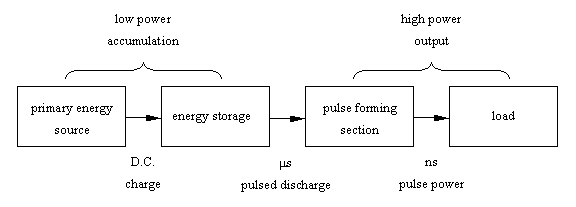
\includegraphics[height=4cm,width=8cm,keepaspectratio=true]{HPMsystem}
 \caption{Primjer ubacivanja slike.}
 \label{fig:prva}
	\end{center}
\end{figure}
\end{verbatim}
Uo�ite uporabu naredbe \verb|\label| unutar bloka. Na nju se potom u tekstu mo�emo referencirati pisanjem npr.\ \verb|Na Slici~\ref{fig:prva}| �ime \LaTeX{} u tekst uvrsti pripadaju�i broj slike, kao npr.\ ``Na Slici~\ref{fig:prva} prikazana je osnovna shema HPM sustava.''
Znak \verb|~| iza rije�i Slici osigurava to�no jedan znak razmaka, �to poma�e ukoliko je rije� Slika na kraju retka, da ne razdvoji rije� Slika i pripadaju�i broj slike.

\begin{figure}[!htbp]
	\begin{center}
 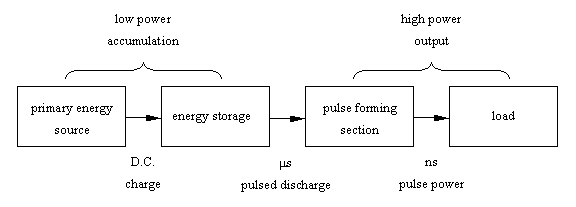
\includegraphics[height=4cm,width=8cm,keepaspectratio=true]{HPMsystem}
 \caption{Primjer ubacivanja slike.}
 \label{fig:prva}
	\end{center}
\end{figure}

Uo�ite i na�in prilago�avanja veli�ine slike. Parametri slike \emph{width} i \emph{height} odre�uju maksimalne dopu�tene dimenzije pri �emu se primarno po�tuje manju navedenu dimenziju, a \emph{keepaspectratio} osigurava zadr�avanje odnosa dimenzija slike, odnosno sprje�ava deformaciju slike, nakon proizvoljno unesenih veli�ina.

Uo�ite da sve oznake tj.\ \emph{labeli} ne smiju imati razmak u imenu. To vrijedi i op�enito, a ne samo za slike.

Tako�er, uo�ite da nije potrebno pisati ekstenziju slike jer to je ure�eno u postavkama glavnoga dokumenta pa time �tedi trud. Ekstenzije koje se mo�e izostaviti su: \emph{jpg}, \emph{jpeg}, \emph{png} i \emph{pdf}.

Shema prikazana na Slici~\ref{fig:prva} �e biti kori�tena i za potrebe idu�ih primjera, a {\color{blue} u mapi na va�em disku ju obri�ite nakon �to po�nete pohranjivati vlastite slike vezane uz va� rad}.


\section{Ubacivanje podslika}
Ponekada se jedna slika sastoji od dvije ili vi�e podslika kojima �elimo opisati neku cjelinu. Slika �e dobiti pripadni broj, a podslike slova (a), (b) itd.
To se mo�e posti�i sljede�om strukturom:
\begin{verbatim}
\begin{figure}[!htpb]
 \begin{center}
  \subfloat[Blok shema HPM sustava.]{\label{fig:HPM}
   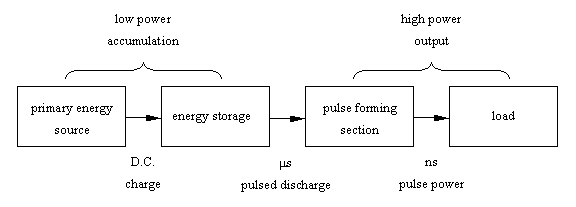
\includegraphics[height=5cm,width=10cm,keepaspectratio=true]{HPMsystem}}\\ 
	    %\hspace{10pt}
   \subfloat[JabRef su�elje za unos ``elektroni�ke'' reference.]
   {\label{fig:jabref}
   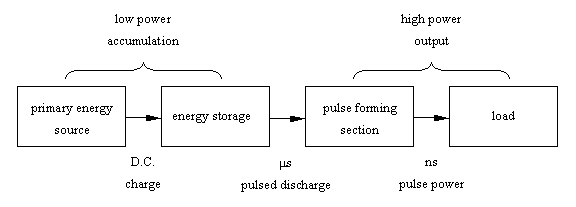
\includegraphics[height=7cm,keepaspectratio=true]{HPMsystem}}
\caption{Primjer ubacivanja vi�e podslika. Ovo je opis cijele slike.}
\label{fig:dvije_podslike}
  \end{center}
\end{figure}
\end{verbatim}
�to �e uvrstiti ono �to se vidi na Slici~\ref{fig:dvije_podslike}, koja se sastoji od dviju podslika.
Podslika~\ref{fig:HPM} pokazuje shemu HPM sustava, a podslika~\ref{fig:jabref} su�elje JabRef programa za unos bibliografskih jedinica.

\begin{figure}[!htpb]
	  \begin{center}
	   \subfloat[Blok shema HPM sustava.]{\label{fig:HPM} 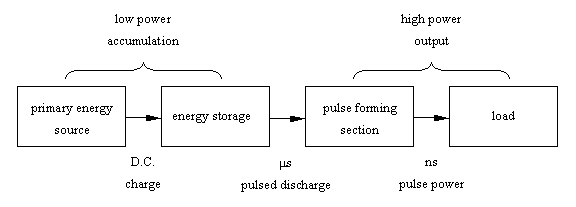
\includegraphics[height=5cm,width=10cm,keepaspectratio=true]{HPMsystem}} \\ %\hspace{10pt}
	   \subfloat[JabRef su�elje za unos ``elektroni�ke'' reference.]{\label{fig:jabref} 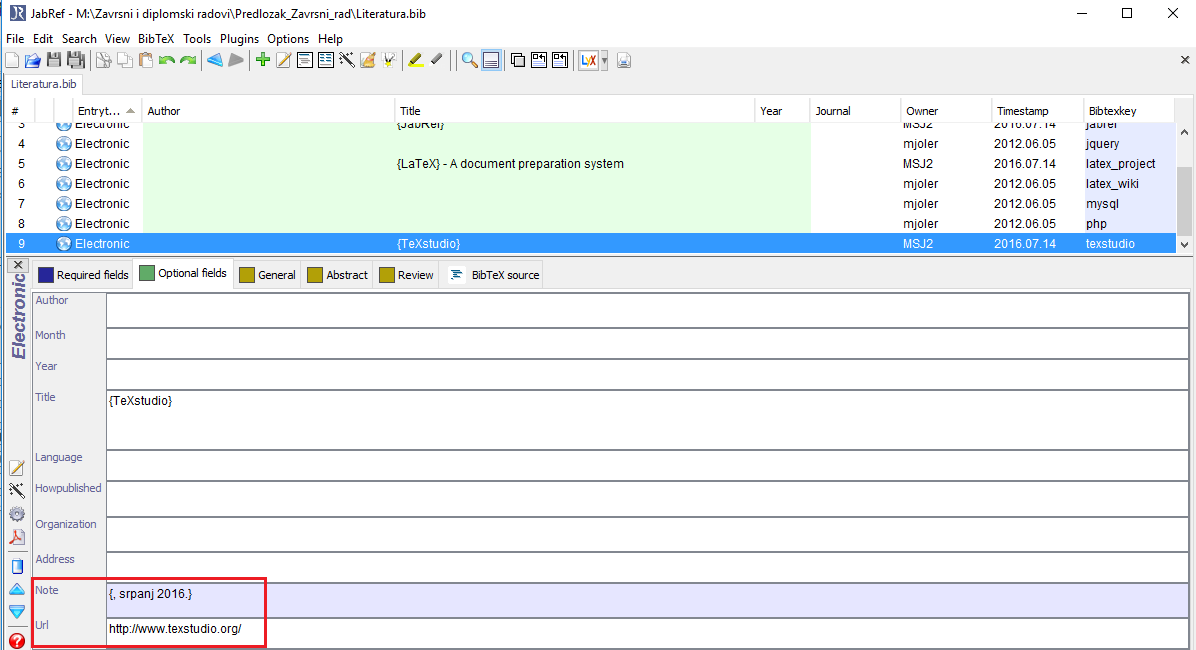
\includegraphics[height=7cm,keepaspectratio=true]{jabref}}
\caption{Primjer ubacivanja vi�e podslika. Ovo je opis cijele slike.}
\label{fig:dvije_podslike}
	  \end{center}
\end{figure}



\section{Ubacivanje tabele} 
Vi�e detalja o kreiranju tabela pro�itajte u literaturi, a sljede�i blok vam omogu�ava kreiranje jednostavne tabele, kao �to je prikazano u Tabeli~\ref{tab:prva}.
\begin{verbatim}
\begin{table}[!htbp]
\renewcommand{\arraystretch}{1.2}
\caption{Ovo je primjer izrade tabele.}
\centering
\begin{tabular}{|c|c|c|}
\hline
variabla & vrijednost 1 & vrijednost 2  \\ [0.5ex]
\hline \hline  
A & 5 & 3 \\ [0.5ex] % razmak do iducega retka
B & 4 & 2 \\ [0.5ex]
\hline
\end{tabular}
\label{tab:prva}
\end{table}
\end{verbatim}

\begin{table}[!htbp]
\renewcommand{\arraystretch}{1.2}
\caption{Ovo je primjer izrade tabele.}
\centering
\begin{tabular}{|c|c|c|}
\hline
variabla & vrijednost 1 & vrijednost 2  \\ [0.5ex]
\hline \hline 
A & 5 & 3 \\ [0.5ex] % razmak do iducega retka
B & 4 & 2 \\ [0.5ex]
\hline
\end{tabular}
\label{tab:prva}
\end{table}
%
Podaci koji su u stupcima se u tabeli razdvajaju znakom \&. Novi redak se na kraju aktualnoga retka formira znakom \verb|\\|. Broj stupaca se definira iza \emph{tabular} time �to se navedu slova koja ozna�avaju poravnavanje teksta u svakom stupcu, a broj slova zna�i broj stupaca koji �e biti kreiran u tabeli. Vertikalni razmak izme�u redaka u tabeli mo�ete za cijelu tabelu prilagoditi uporabom sljede�e sintakse prije strukture za tabelu:\\
\verb| \renewcommand{\arraystretch}{1.2} | gdje broj u zagradi na kraju (ovdje je 1.2) prilagodite sukladno va�oj preferenciji. Mo�e se prilagoditi i razmak za svaki pojedini redak (uo�ite \verb|[0.5ex]| na kraju redaka), ali to je manje od interesa jer tipi�no �elimo da svi retci imaju jednaki razmak jedni od drugih.

Sli�no mo�ete u�initi i za razmak izme�u stupaca tabele navo�enjem sljede�e sintakse prije bloka tabele:\\
\verb| \renewcommand{\tabcolsep}{0.3cm} |.



\section{Uporaba kratica u tekstu. Automatsko generiranje popisa kratica.}  \label{sec:kratice}
Listu kratica definirajte u datoteci \verb|Kratice.tex| (vidjeti predlo�ak unutar datoteke). U redovitom tekstu, kraticu  mo�ete ubaciti kori�tenjem naredbe \verb|\gls{ID_kratice}| gdje je \verb|ID_kraticE| identifikator kratice kako je definiran u datoteci \emph{Kratice.tex}. Pri prvoj uporabi naredbe \verb|\gls|, ispisat �e se najprije puni naziv pojma pa u zagradi kratica, a kod svake sljede�e uporabe, ispisat �e se samo kratica. Na primjer, kada (nakon prethodnog deklariranja u datoteci \verb|Kratice.tex|) upotrijebite \verb|\gls{gsm}| prvi puta, u tekstu �e se ispisati \gls{gsm}, a kada upotrijebite \verb|\gls{gsm}| drugi puta i dalje, u tekstu �e se ispisati samo \gls{gsm} (usporedi s definicijom kratice u datoteci \verb|Kratice.tex|). 
 
{\color{red} Listu kratica generirate sljede�im postupkom:} \label{generiranje_liste_kratica}
\begin{enumerate}
	\item Pokrenite kompilaciju cijeloga teksta jedanputa (to �e generirati neke datoteke koje su potrebne za daljnju obradu, specifi�no one s ekstenzijama .ist i .glo).
	\item Otvorite \emph{Command Prompt} aplikaciju na va�em ra�unalu i postavite se u radnu mapu gdje su vam datoteke za diplomski rad. 
	\item Potom pokrenite \emph{makeindex} rutinu (ona �e tipi�no biti ve� prisutna na va�em ra�unalu) upisuju�i sljede�u sintaksu: \\
	\verb|makeindex   -s myDoc.ist  -o myDoc.gls   myDoc.glo| \\
	gdje naziv datoteke \emph{myDoc} treba zamijeniti nazivom va�e glavne .tex datoteke, (npr. \verb|JMBAG_Ime_Prezime.tex|).
	\item Pokrenite \LaTeX{} jo� jednom ili dva puta, ako treba, dok se u uvodu pdf dokumenta ne pojavi lista kratica (pod naslovom \emph{Pojmovnik}).	
\end{enumerate}

Mo�da isprva zvu�i slo�eno, ali zapravo nije (bar ne uz ovako precizne upute!). Svaki puta kada dodate nove definicije kratica, potrebno je ponoviti ovaj postupak da bi se a�urirale odgovaraju�e datoteke i uredno prikazala potpuna lista u pdf-u (a i izbjegle poruke o pogre�kama tijekom kompajliranja teksta). 

Nije te�ko nakon �to prvi puta pro�ete ovaj postupak i omogu�ava vam u tekstu biti dosljedan u uporabi odre�ene kratice. Da izbjegnete �u�enje, va�no je jo� re�i da �e se ovim postupkom automatski stvoriti tek lista kratica koje ste u tekstu upotrijebili uporabom sintakse \verb|\gls|, a ne na temelju liste definicija koje ste naveli u datoteci \verb|Kratice.tex|. Zato, ako nijednom u tekstu ne upotrijebite sintaksu \verb|\gls|, ne�e biti ispisan ni popis kratica tj.\ \emph{Pojmovnik}. {\color{blue} Kako \LaTeX{} na kraju uvijek nagradi trud koji je ulo�en u savladavanje njegove sintakse, pogodnost ovakvoga automatskoga kreiranja Pojmovnika je i to �to uz svaki kraticu \LaTeX{} automatski ispi�e i brojeve stranica na kojima se doti�na kratica pojavljuje!} U elektroni�kom pdf dokumentu, brojevi stranica su ujedno i hiper-veze na te stranice pa se tako mo�e odmah sko�iti na stranicu gdje je pojedina kratica upotrijebljena.

Ukoliko vam se prethodno opisani postupak �ini preslo�enim, popis kratica mo�ete napraviti i ru�no, isto pomo�u datoteke Kratice.tex, u kojoj tako�er postoji kratki predlo�ak i za takav pristup. Za to je onda u osnovnoj datoteci \verb|JMBAG_Ima_Prezime.tex| potrebno deaktivirati liniju koda koja po�inje sa \verb|\printglossary|, a aktivirati blok koji po�inje sa \verb|\begin{glossary}| i zavr�ava sa \verb|end{glossary}|.



\section{Nagla�avanje teksta}
\subsection{Navodnici}
Za navodnike s lijeve strane fraze (otvaranje navodnika) koristi se 2x jednostruki navodnik koji se na tipkovnici nalazi lijevo od broja 1, a za navodnike s desne strane fraze (zatvaranje navodnika), koristi se 2x jednostruki navodnik koji se na tipkovnici nalazi na tipki \emph{�}, �to proizvede npr.\ ``abc''.

{\color{blue} Alternativno, u ovom paketu je pripremljena i naredba {\color{red} \verb|\navod{abc}|} gdje je \emph{abc} tekst koji se stavlja izme�u navodnika, tj.\ \navod{abc}.}

\subsection{Kosa i podebljana slova}
Nagla�avanje neke rije�i ili fraze pomo�u kosih (italic) slova mo�emo dobiti uporabom naredbe {\color{red} \verb|\emph{abc}|} ili pomo�u  {\color{red}\verb|\textit{abc}|} gdje je \emph{abc} neki tekst koji se �eli naglasiti.

\textbf{Podebljana slova} mo�emo posti�i uporabom naredbe {\color{red} \verb|\textbf{abc}|} gdje je \textit{abc} neki tekst koji �elimo podebljati.

\section{Verbatim: okru�enje za doslovni tekst}
Verbatim okru�enje omogu�ava ispis teksta u izvornom obliku, bez da ga \LaTeX{} tuma�i po svojiim sintakti�kim pravilima. To je pogodno kada se na stranicu  npr.\ �eli kopirati dio programskoga koda iz nekog jezika i kada �elimo zadr�ati sve izvorne znakove u nekoj frazi, bez da \LaTeX{} po�ne javljati pogre�ke kod kompajliranja, �to bi se moglo pojaviti kada se ne bi koristilo \emph{verbatim okru�enje}, po�to bi neke znakove interpretirao kao pogre�ke u sintaksi.

Postoji kra�i i du�i oblik verbatima. Kra�i slu�i za kra�u frazu od jedne ili par rije�i, a du�i za vi�e redaka.

\noindent Kra�i oblik verbatima ima sintaksu: \verb+\verb|neka fraza|+

\noindent Du�i oblik verbatima ima sintaksu:\\
\verb|\begin{verbatim}| \\
\verb|neki tekst| \\
\verb|\end{verbatim}| \\


\section{Kreiranje jedne jednad�be ili serije jednad�ba}

\subsection{Kreiranje jedne jednad�be}
Jednad�ba se napi�e u posebnom matemati�kom modu koji se kreira pomo�u bloka:
\begin{verbatim}
	\begin{equation}
		 A = B + C   \label{eq:prva}
	\end{equation}
\end{verbatim}
�to �e dati sljede�i izgled:
\begin{equation}
	 A = B + C   \label{eq:prva}
\end{equation}
Da bi se na nju referenciralo, na �eljenom mjestu u tekstu upi�emo \verb|\eqref{eq:prva}|, �ime �e se uvrstiti njezin pripadni (automatski generirani) broj, a za potpuniji smisao mo�emo npr.\ napisati \verb| Jednad�ba~\eqref{eq:prva}|, rezultat �ega je da �e u tekstu pisati Jednad�ba~\eqref{eq:prva}. 
Ako ju se ne �eli numerirati, onda se nakon rije�i \emph{begin} stavi zvjezdica, tj.\ \verb|begin*{equation}|.

\subsection{Kreiranje grupe jednad�ba}
Grupa jednad�ba se kreira uporabom \emph{subequations} sintakse. Na primjer, sljede�i blok �e definirati dvije podjednad�be u grupi, gdje �e svaka biti numerirana istim brojem, a razlikovati slovom iza broja.
\begin{verbatim}
	\begin{subequations}
		\begin{align}
		        A &= B + C  	\label{subeq:prva} \\
		        D &= F + G		\label{subeq:druga}
		\end{align}
	\label{subeq:obje}
	\end{subequations}
\end{verbatim}

To �e u izlaznom dokumentu rezultirati sljede�im izgledom:
\begin{subequations}
\begin{align}
        A &= B + C  	\label{subeq:prva} \\
        D &= F + G		\label{subeq:druga}
\end{align}
\label{subeq:obje}
\end{subequations}
U \eqref{subeq:prva} je prikazano dobivanje vrijednosti $A$, a u \eqref{subeq:druga} je prikazano dobivanje vrijednosti $D$. Jednad�ba~\eqref{subeq:obje} je \emph{�uveni studentov zakon}!



\section{Liste}
Liste su �este forme u tekstu kojima se na pregledni na�in nabrajaju neke stavke. Stavke obi�no navodimo ili s to�kama na po�etku, s brojevima ili sa slovima. U \LaTeX-u su upravo ta tri stila unaprijed definirana, a mogu�e su i slo�enije definicije stilova i kombinacije lista.

\subsection{Lista s to�kama}
Lista s to�kama se postigne blokom
\begin{verbatim}
\begin{itemize}
    \item prva nenumerirana stavka
    \item druga nenumerirana stavka
\end{itemize}
\end{verbatim}
�to na ekranu proizvede:
\begin{itemize}
% \setlength\itemsep{1ex}   % za lokalnu prilagodbu
	\item prva nenumerirana stavka
	\item druga nenumerirana stavka
\end{itemize}

\subsection{Lista s brojevima}
Numerirana lista s brojevima se postigne blokom
\begin{verbatim}
\begin{enumerate}[itemsep=1ex, topsep=4pt, partopsep=0pt]
     \item prva numerirana stavka
     \item druga numerirana stavka
\end{enumerate}
\end{verbatim}
U uglatoj zagradi su tri parametra kojima se to�no mo�e kontrolirati vertikalni razmak izme�u stavki u listi (\emph{itemsep}), razmak izme�u prethodnoga teksta i prve stavke u listi (\emph{topsep}) i dodatni prostor izme�u liste i prethodnoga paragrafa kada lista zapo�inje novi paragraf (\emph{partopsep}), ali te parametre \textbf{ne morate navoditi} tj.\ tu uglatu zagradu ne morate pisati. Tada �e se primijeniti vrijednosti parametara koje su definirane za cijeli dokument, a ove parametre se mo�e upotrijebiti tek da u nekom pojedinom slu�aju prilagodite razmake.
Za osjetiti efekte ovih parametara, najbolje se malo sam poigrati razli�itim vrijednostima parametara i vidjeti posljedice toga na listu (pri tome se uz brojeve kao prikladne jedinice za razmak mogu koristiti \emph{pt}, \emph{ex} ili \emph{em}).

\subsection{Proizvoljno ozna�ena lista}
Takva se lista mo�e posti�i u sklopu op�enitije forme koja omogu�uje proizvoljni opis ispred pojedine stavke, pomo�u sljede�ega bloka:
\begin{verbatim}
\begin{description}
     \item[a)] prva opisna stavka
     \item[b)] druga opisna stavka
\end{description}
\end{verbatim}
�to na ekranu proizvede:
\begin{description}%[itemsep=1ex, topsep=4pt, partopsep=0pt] za lokalnu prilagodbu
	\item[a)] prva opisna stavka
	\item[b)] druga opisna stavka \\
\end{description}
%
Kod ove strukture, u uglatu zagradu iza naredbe \verb|\item|, navodi se proizvoljna oznaka kojom se �eli na neki na�in ``numerirati'' listu.
%:::::::::::::::::::::::::::::::::::::::::::::::::::
\chapter{Dodatne informacije}
\section{Primjeri uporabe sintakti�kih struktura}
\begin{enumerate}
	\item Za uvid u kontekstualnu primjenu raznih sintakti�kih struktura, mo�ete otvoriti datoteku \href{run:Intro.tex}{{\color{blue}Intro.tex}}, unutar koje su napisane i ove upute. 
	\item Primjere slo�enijih sintakti�kih struktura, kao �to su ubacivanje slike, tabele ili jednad�be, mo�ete na�i u datoteci \href{run:sintaksa_cestih_struktura.tex}{{\color{blue}sintaksa\_cestih\_struktura.tex}} koja je dio paketa. Odabrane se strukture mo�e kopirati i zalijepiti u va� tekst, uz minimalne prilagodbe kao �to su naziv slike, veli�ina slike, opis i ID slike, a analogno i za tabele i jednad�be.
	\item Kona�no, za vi�e detalja o bilo �emu, potra�ite informacije u dvama priru�nicima koji su prilo�eni u mapi \href{run:prirucnici}{{\color{blue}prirucnici}} ili na webu, gdje se, me�u obiljem drugih informacija, nalaze i korisne wiki stranice \cite{latex_wiki,tex_exchange} o \LaTeX-u pomo�u kojih se obi�no brzo prona�e upute i zadovoljavaju�e rje�enje kakvom sintaksom se mo�e urediti �eljeni dio teksta.
\end{enumerate}

\section{Savjeti za lak�e ure�ivanje teksta}
Vjerujem da vam ovaj dokument mo�e uvelike pomo�i u pripremi teksta va�ega zavr�nog/diplomskog rada i omogu�iti da glavninu vremena tro�ite na sadr�aj rada, a manje na formatiranje rada jer to �e za vas sada obaviti \LaTeX{}! 

No, korektnosti radi, potrebno je napomenuti i sljede�e: \LaTeX{} je vrlo osjetljiv na pogre�ke u sintaksi naredbi (da, ba� kao �to su i programski jezici) pa vas mo�e povremeno ugnjaviti javljanjem pogre�ke koju nikako ne uspijevate uo�iti gdje je. Iskustvo kojim se izbjegava ta nelagoda jest sljede�e:
\begin{itemize}
	\item svako poglavlje napi�ite u novoj datoteci (da biste koli�inu teksta razdvojili na preglednije i manje cjeline) koju imenujte prikladnim imenom (bez razmaka u imenu). Potom te datoteke samo pozivajte iz glavnoga dokumenta \verb|JMBAG_Ime_Prezime.tex| pomo�u naredbe \verb|\include{ime_datoteke}|. Takav je pristup upravo i kori�ten u pripremi ovoga paketa.
	%
	\item {\color{red} budite koncentrirani dok pi�ete \LaTeX{} naredbe, poglavito zagrade, posebne znakove i matemati�ki tekst gdje se zahtijeva uporaba znaka \$!}
	%
	\item kompajlirajte tekst prije nego se skupi puno teksta jer tako �ete imati manje teksta za prekontrolirati u slu�aju pogre�ke. Tako�er vam za provjeru tek manjega dijela dokumenta mo�e pomo�i paket \verb|\usepackage{syntonly}| i naredba \verb|syntaxonly|, a isto tako i naredba \verb|\includeonly{ime_datoteke}| kojom �ete kompajlirati samo tu navedenu datoteku, �ime  ispred ``ne�eljenih'' datoteka ne morate stavljati znak ``komentara'' (\%).
	%
	\item ako niste sigurni ho�e li vam raditi neka naredba nakon pisanja, radije tekst kompajlirajte odmah po pisanju te naredbe---da vidite �to �ete dobiti i rije�ite dvojbu, nego da �ekate da se skupi jo� dubioznih mjesta u tekstu, kada �e nakon kompajliranja biti te�e detektirati koja linija teksta zapravo izaziva probleme (\LaTeX-ov prozor s porukama �esto nije odve� precizan u lociranju i opisu pogre�aka, ovisno o editoru teksta koji koristite).
\end{itemize}


\section{Zavr�ne napomene}
Ovime zaklju�ujemo uvodne upute koje �e najve�em broju studenata biti dovoljne (ili barem dovoljna osnova) za uspje�no pisanje zavr�nog odnosno diplomskog rada.

Prije nego prije�ete na kreiranje vlastitoga sadr�aja u�inite jo� sljede�e akcije kojima �ete deaktivirati dio paketa koji �e biti nepotreban:
\begin{enumerate}
	\item u mapi \href{run:slike}{{\color{blue}slike}}, obri�ite datoteke \verb|HPMsystem.png| i \verb|jabref.png| jer su one slu�ile tek za ilustracije u ovim Uputama.
	%
	\item u glavnoj datoteci  \href{run:JMBAG\_Ime\_Prezime.tex}{{\color{blue}JMBAG\_Ime\_Prezime.tex}} stavite znak komentara ``\%'' ispred linije \verb|\include{Intro}| kojom se pozivaju ove upute ili obri�ite tu liniju koda, �ime to vi�e ne�e biti uklju�eno u tekst va�eg vlastitoga rada.
\end{enumerate}

Budite slobodni emailati svoje dojmove o razumljivosti i prakti�nosti ovoga materijala, kao i informacije o uo�enim pogre�kama u tekstu. \\

\noindent Ugodan rad! \\

\noindent Miroslav Joler	\\	
\href{mailto:mjoler@riteh.hr}{mjoler@riteh.hr}	\\ \\


{\color{red} A sada, prije�ite na kreiranje vlastitoga sadr�aja, pri �emu �e vam, za po�etak, pomo�i vodi� iz sljede�ega poglavlja.}


\chapter{Vodi� za pisanje vlastitoga teksta}

\section{Upis uvodnih podataka}
\begin{enumerate}
	\item {\color{red} \textbf{Otvaranje glavne datoteke.}} Pokrenite va� editor \LaTeX{} teksta i iz njega otvorite sredi�nju datoteku ovoga predlo�ka za pisanje rada, koja je nazvana \href{run:JMBAG\_Ime\_Prezime.tex}{{\color{blue}JMBAG\_Ime\_Prezime.tex}} i nalazi se u sredi�njoj mapi unutar ovoga paketa (ili probajte klikom na prethodnu poveznicu u tekstu).
	%
	\item {\color{red} \textbf{Upis uvodnih podataka.}} U gornjem dijelu dokumenta nemate ni�ta za mijenjati, nego skrolajte prema dolje do linije koja glasi: \verb|\begin{document}|. Specifi�ni podaci koje student/ica nakon toga treba upisati bit �e uz sljede�e naredbe:
	\begin{itemize}
		\item \verb|\degreesubject|: upisati razinu studija koji poha�ate (npr.\ Preddiplomski studij ra�unarstva ili Diplomski studij ra�unarstva i sl.)
		\item \verb|\documenttype|: upisati \emph{Zavr�ni rad} ili \emph{Diplomski rad}
		\item \verb|\title|: upisati naslov rada kako je zadano u slu�benom zadatku
%\item \verb|\date|: upisati samo mjesec predaje rada. Godina se upisuje automatski.
		\item \verb|\author|: upisati svoje ime i prezime
		\item \verb|\jmbag|: zamijeniti postoje�i broj vlastitim JMBAG brojem 
		\item \verb|\mentor|: upisati titulu te ime i prezime svojega mentora
	\end{itemize}
	%
	\item {\color{red} \textbf{Prva kompilacija teksta.}} \label{encoding2} \textbf{POZOR: prije prve kompilacije teksta, uvjerite se da vam je kodna stranica postavljena na ``windows-1250'' (alternativni naziv: ``cp1250''). Ona je kod kompilacije klju�na za ispravno ispisivanje hrvatskih dijakriti�kih znakova u izlaznom PDF dokumentu! Vidite stranicu~\pageref{encoding1} za dodatne upute o postavljanju te kodne stranice.} 
	
	Za prvu probu nakon une�enih podataka, kompajlirajte dokument na na�in da unutar va�ega \emph{TeXstudio} editora odaberete opciju izbornika \emph{Tools} koja je nazvana \emph{Build \& View} ili, kra�e, samo stisnete tipku F5 ili kliknete na ikonu dvostrukog zelenog trokuta u glavnoj traci alata. To pokrene postupak kompajliranja svega i rezultat bi trebao biti \emph{PDF} datoteka u kojoj �ete vidjeti lijepo formatirane po�etne stranice rada. \\
	Za prvu kompilaciju budite strpljivi jer \LaTeX{} �e mo�da tijekom postupka kompilacije povla�iti neke vanjske pakete koji mu trebaju, a nisu jo� prisutni na va�em ra�unalu nakon instalacije \LaTeX-a. U takvom slu�aju, tipi�no se dovoljno strpjeti oko 30~s prije nego se pojavi PDF dokument kao rezultat kompilacije. Ukoliko se to ne dogodi, u prozoru s porukama �e vam \LaTeX{} mo�ebitno napisati da mu nedostaje neka datoteka sa .sty ekstenzijom, �to zna�i da automatsko povla�enje ili nije namje�teno kao opcija u va�oj \LaTeX{} instalaciji (ali mo�e se namjestiti u postavkama \LaTeX-a) ili nije uspjelo pa tra�eni paket mo�ete sami na webu potra�iti i povu�i na va�e ra�unalo (najjednostavnije je uvrstiti ga u glavnu mapu va�ega projekta). Pozor: 
		\begin{itemize}
			\item TeXstudio u startu ve� ima postavljen \emph{PDF} kao format izlaznoga dokumenta, ali ukoliko to iz nekog razloga ne bude slu�aj, mo�e se postaviti u izborniku i opcijama za konfiguraciju TeXstudia. 
			%
			\item ponekada je potrebno 2-3 puta pokrenuti \emph{Build} operaciju da bi sve promjene bile a�urirane u \emph{PDF} dokumentu kao �to su npr.\ brojevi referenca, popis literature i sl. (TeXstudio, po potrebi, �esto sam automatski pokrene kompajliranje dva puta zaredom, ali po�to to ne mora biti slu�aj svaki puta, dobro je za znati pa onda vi ru�no pokrenete drugi puta.)
		\end{itemize}
	%
	\item {\color{red} \textbf{Promjena naziva glavne datoteke.}} Zatvorite \verb|JMBAG_Ime_Prezime.tex| datoteku (i svaku drugu ako je jo� neka \emph{tex} datoteka otvorena) i u mapi {\color{red} promijenite ime \verb|JMBAG_Ime_Prezime.tex| datoteke} na na�in da {\color{red} JMBAG, ime i prezime zamijenite va�im specifi�nim podacima}. Potom ponovo otvorite tu datoteku jer ona je sredi�nja datoteka koja slu�i za kompajliranje cijeloga projekta i mora biti otvorena uvijek kada se kompajlira tekst (drugim rije�ima, tu datoteku kompajlirate). \textbf{(Nakon �to idu�i put kompjalirate projekt pod novim imenom, obri�ite u va�oj radnoj mapi sve datoteke koje nose staro ime!)}
	%
	\item {\color{red} \textbf{Definiranje \emph{Posvete}.}} (Neobavezno). Ako �elite napisati kratku posvetu (pazi, posveta nije isto �to i zahvala, koju imate priliku definirati nakon toga) nekome (majci, ocu, roditeljima i sl.), u glavnoj datoteci va�ega rada (stari naziv \verb|JMBAG_Ime_Prezime.tex| koji ste zamijenili novim nazivom) prona�ite blok koji po�inje tekstom \verb|\begin{dedication}| i u liniji ispod toga tekst predlo�ka zamijenite nekim va�im tekstom suvisle posvete. \\
	Ukoliko nemate potrebu upisati neku Posvetu, u tom slu�aju (o)stavite znakove komentara \verb|%| ispred te tri linije koda, da biste to deaktivirali kod kompilacije teksta.
	%
	\item {\color{red} \textbf{Definiranje \emph{Zahvale}.}} (Neobavezno). Ako �elite napisati zahvalu nekome (npr.\ mentoru za savjete, roditeljima ili bliskoj osobi za potporu tijekom studija, kolegama za pomo� pri radu i sl.), otvorite datoteku \href{run:Zahvala.tex}{{\color{blue}Zahvala.tex}} i zamijenite tekst predlo�ka nekim va�im osobnim tekstom. Ostale linije predlo�ka ne mijenjajte. Potom snimite datoteku (Ctrl+S) i zatvorite.\\ 
	Ukoliko nemate potrebu pisati neku zahvalu, prona�ite u glavnoj datoteci blok koji po�inje tekstom \verb|\begin{acknowledgments}| i sve linije toga bloka stavite u komentar. \\
	Naknadne izmjene i prilagodbe teksta Zahvale mo�ete u�initi izmjenama u datoteci \verb|Zahvala.tex|, a aktiviranje ili deaktiviranje teksta Zahvale uklanjanjem ili postavljanjem komentara na taj blok koda u glavnoj datoteci.
	%
	\item {\color{red} \textbf{Ure�enje \emph{Izjave o samostalnoj izradi rada}.}} (Obavezno). Otvorite datoteku \href{run:Izjava.tex}{{\color{blue}Izjava.tex}} i:
	\begin{enumerate}
		\item po �elji, prilagodite tekst izjave s obzirom na rod glagola (``izradio'' ili ``izradila'')
		\item  u retku gdje pi�e \verb|Ime Prezime|, umjesto toga upi�ite svoje ime i prezime.
		\item pomo�u linije \verb+\verb|  |+ regulirajte poravnanje imena i prezimena s gornjom crtom.
	\end{enumerate}
	Snimite datoteku na disk i zatvorite.
\end{enumerate}

\section{Po�etak pisanja glavnoga dijela rada}
\begin{enumerate}
	\item {\color{red} \textbf{Pisanje prvoga poglavlja.}} Otvorite datoteku  \href{run:Poglavlje\_1.tex}{{\color{blue}Poglavlje\_1.tex}} i po�nite pisati svoj vlastiti tekst uz postavljanje naslova poglavlja i sekcija (tj. potpoglavlja) po vlastitom izboru, a na kraju proizvoljno mo�ete promijeniti ime te datoteke u ne�to �to odgovara sadr�aju va�ega poglavlja i to ime stavite u \verb|\include| naredbu umjesto inicijalnoga naziva \verb|Poglavlje_1| (ako vas ne smeta, mo�ete i ostaviti naziv \verb|Poglavlje_1|).\\ Da bi se tekst toga \verb|Poglavlja_1| uspje�no kompajlirao u izlazni dokument, uklonite znak komentara ``\%'' ispred \verb|\include{Poglavlje_1}| naredbe u glavnoj datoteci (stari naziv datoteke bio je  \href{run:JMBAG\_Ime\_Prezime.tex}{{\color{blue}JMBAG\_Ime\_Prezime.tex}}). Tako u�inite i za sva nova poglavlja koja �ete potom kreirati.
	%
	\item {\color{red} \textbf{Definiranje \emph{Literature.}}} Popis literature se gradi sukcesivno tijekom pisanja rada. Kao �to je opisano u Sekciji~\ref{sec:RefLit} na stranici \pageref{sec:RefLit}, popis literature mo�ete graditi na dva na�ina---sa i bez uporabe JabRef programa, a oba na�ina su omogu�ena u datoteci \href{run:Literatura.tex}{{\color{blue}Literatura.tex}}.\\ 
	Za onaj na�in za koji ste se odlu�ili, uklonite komentare ispred toga bloka naredbi u datoteci \verb|Literatura.tex|, a za onaj drugi na�in postavite znakove komentara, da biste taj drugi na�in onesposobili kod kompajliranja teksta.\\
	\emph{Spoznajte da se u popisu literature smiju na�i samo one stavke koje su referencirane u radu}! Drugim rije�ima, ne mo�ete definirati popis literature, a da se na pojedinu stavku nijednom ne referencirate u tekstu rada! S druge strane, na pojedinu se literaturu mo�ete u radu referencirati koliko god puta ho�ete, ali u popisu literature ju se navodi samo jedanput!
	
	{\color{red} POZOR: ponekada se dogodi da postupak kompajliranja teksta (tvrdoglavo) ne�e osvje�iti popis literature nakon �to je u njemu bilo izmjena (npr. redoslijed stavki, redni brojevi i sl.), �ak ni nakon dvaju pokretanja kompajlera. \textbf{Tada je najbolje obrisati pomo�ne datoteke (me�u kojima je i \emph{.bbl} datoteka koja je ``zadu�ena'' za popis literature) uporabom naredbe ``Clean Auxiliary Files\dots'', koja se nalazi pod izbornikom \emph{Tools}, pa ponovo pokrenuti kompajler dva puta.}} Brisanje pomo�nih datoteka ima efekt ``�istoga starta'' i uglavnom �e dati �eljeni rezultat, a kada ni to ne bi pomoglo, onda se mo�e ru�nim intervencijama u datoteci \emph{.bbl} izvr�iti potrebne promjene.
	%
	\item {\color{red} \textbf{Definiranje \emph{kratica}}} za pojmove kori�tene u tekstu (neobavezno). Kratice i pripadaju�e pune nazive pojmova definirajte u datoteci \href{run:Kratice.tex}{{\color{blue}Kratice.tex}}, prema po�etnom predlo�ku koji je u njoj dan. Listu mo�ete sukcesivno pro�irivati svaki puta kada na�ete potrebu definirati neki novi pojam s kraticom.\\
	Uporaba kratica u tekstu je opisana u Sekciji~\ref{sec:kratice}, ali popis kratica (u tekstu zvan \emph{Pojmovnik}) ne�e automatski biti pro�iren novim kraticama, ve� za to trebate provesti postupak za \hyperref[generiranje_liste_kratica]{{\color{blue} generiranje liste kratica}} koji je opisan u Sekciji~\ref{sec:kratice}.
	%
	\item {\color{red} \textbf{Pisanje ostalih dijelova rada.}} Nastavite pisati rad definiranjem \emph{Poglavlja~2}, \emph{Poglavlja~3} itd.\, analogno kako ste �inili za \emph{Poglavlje~1}\dots
	%
	\item {\color{red} \textbf{Upis Sa�etka rada.}}\\
	Na kraju rada, a prije mo�ebitnih (neobaveznih) priloga, potrebno je napisati \emph{Sa�etak} rada i \emph{klju�ne rije�i} na hrvatskom i engleskom (gdje je to naslovljeno s \emph{Abstract} odnosno \emph{keywords}). \\
	Sa�etak je forma kratkoga teksta (1-3 paragrafa ukupne du�ine manje od pola stranice) u kojemu navedete \emph{�to} je u radu prikazano i \emph{ne ulazite u daljnja obja�njavanja}.\\
	Za upis \emph{Sa�etka} i \emph{klju�nih rije�i} odnosno \emph{Abstract}-a i \emph{keywords}-a, otvorite datoteku \href{Sazetak.tex}{{\color{blue}Sazetak.tex}} i tekst predlo�ka zamijenite vlastitim tekstom sa�etaka i klju�nih rije�i na hrvatskom i engleskom, a ostatak strukture koda nemojte mijenjati.
\end{enumerate}

\vspace{10pt}

\begin{flushright}
	Sretno! \\
	Miroslav Joler \\
	\href{mailto:mjoler@riteh.hr}{mjoler@riteh.hr}
\end{flushright}

| kojom se pozivaju ove upute ili obri�ite tu liniju koda, �ime to vi�e ne�e biti uklju�eno u tekst va�eg vlastitoga rada.
\end{enumerate}

Budite slobodni emailati svoje dojmove o razumljivosti i prakti�nosti ovoga materijala, kao i informacije o uo�enim pogre�kama u tekstu. \\

\noindent Ugodan rad! \\

\noindent Miroslav Joler	\\	
\href{mailto:mjoler@riteh.hr}{mjoler@riteh.hr}	\\ \\


{\color{red} A sada, prije�ite na kreiranje vlastitoga sadr�aja, pri �emu �e vam, za po�etak, pomo�i vodi� iz sljede�ega poglavlja.}


\chapter{Vodi� za pisanje vlastitoga teksta}

\section{Upis uvodnih podataka}
\begin{enumerate}
	\item {\color{red} \textbf{Otvaranje glavne datoteke.}} Pokrenite va� editor \LaTeX{} teksta i iz njega otvorite sredi�nju datoteku ovoga predlo�ka za pisanje rada, koja je nazvana \href{run:JMBAG\_Ime\_Prezime.tex}{{\color{blue}JMBAG\_Ime\_Prezime.tex}} i nalazi se u sredi�njoj mapi unutar ovoga paketa (ili probajte klikom na prethodnu poveznicu u tekstu).
	%
	\item {\color{red} \textbf{Upis uvodnih podataka.}} U gornjem dijelu dokumenta nemate ni�ta za mijenjati, nego skrolajte prema dolje do linije koja glasi: \verb|\begin{document}|. Specifi�ni podaci koje student/ica nakon toga treba upisati bit �e uz sljede�e naredbe:
	\begin{itemize}
		\item \verb|\degreesubject|: upisati razinu studija koji poha�ate (npr.\ Preddiplomski studij ra�unarstva ili Diplomski studij ra�unarstva i sl.)
		\item \verb|\documenttype|: upisati \emph{Zavr�ni rad} ili \emph{Diplomski rad}
		\item \verb|\title|: upisati naslov rada kako je zadano u slu�benom zadatku
%\item \verb|\date|: upisati samo mjesec predaje rada. Godina se upisuje automatski.
		\item \verb|\author|: upisati svoje ime i prezime
		\item \verb|\jmbag|: zamijeniti postoje�i broj vlastitim JMBAG brojem 
		\item \verb|\mentor|: upisati titulu te ime i prezime svojega mentora
	\end{itemize}
	%
	\item {\color{red} \textbf{Prva kompilacija teksta.}} \label{encoding2} \textbf{POZOR: prije prve kompilacije teksta, uvjerite se da vam je kodna stranica postavljena na ``windows-1250'' (alternativni naziv: ``cp1250''). Ona je kod kompilacije klju�na za ispravno ispisivanje hrvatskih dijakriti�kih znakova u izlaznom PDF dokumentu! Vidite stranicu~\pageref{encoding1} za dodatne upute o postavljanju te kodne stranice.} 
	
	Za prvu probu nakon une�enih podataka, kompajlirajte dokument na na�in da unutar va�ega \emph{TeXstudio} editora odaberete opciju izbornika \emph{Tools} koja je nazvana \emph{Build \& View} ili, kra�e, samo stisnete tipku F5 ili kliknete na ikonu dvostrukog zelenog trokuta u glavnoj traci alata. To pokrene postupak kompajliranja svega i rezultat bi trebao biti \emph{PDF} datoteka u kojoj �ete vidjeti lijepo formatirane po�etne stranice rada. \\
	Za prvu kompilaciju budite strpljivi jer \LaTeX{} �e mo�da tijekom postupka kompilacije povla�iti neke vanjske pakete koji mu trebaju, a nisu jo� prisutni na va�em ra�unalu nakon instalacije \LaTeX-a. U takvom slu�aju, tipi�no se dovoljno strpjeti oko 30~s prije nego se pojavi PDF dokument kao rezultat kompilacije. Ukoliko se to ne dogodi, u prozoru s porukama �e vam \LaTeX{} mo�ebitno napisati da mu nedostaje neka datoteka sa .sty ekstenzijom, �to zna�i da automatsko povla�enje ili nije namje�teno kao opcija u va�oj \LaTeX{} instalaciji (ali mo�e se namjestiti u postavkama \LaTeX-a) ili nije uspjelo pa tra�eni paket mo�ete sami na webu potra�iti i povu�i na va�e ra�unalo (najjednostavnije je uvrstiti ga u glavnu mapu va�ega projekta). Pozor: 
		\begin{itemize}
			\item TeXstudio u startu ve� ima postavljen \emph{PDF} kao format izlaznoga dokumenta, ali ukoliko to iz nekog razloga ne bude slu�aj, mo�e se postaviti u izborniku i opcijama za konfiguraciju TeXstudia. 
			%
			\item ponekada je potrebno 2-3 puta pokrenuti \emph{Build} operaciju da bi sve promjene bile a�urirane u \emph{PDF} dokumentu kao �to su npr.\ brojevi referenca, popis literature i sl. (TeXstudio, po potrebi, �esto sam automatski pokrene kompajliranje dva puta zaredom, ali po�to to ne mora biti slu�aj svaki puta, dobro je za znati pa onda vi ru�no pokrenete drugi puta.)
		\end{itemize}
	%
	\item {\color{red} \textbf{Promjena naziva glavne datoteke.}} Zatvorite \verb|JMBAG_Ime_Prezime.tex| datoteku (i svaku drugu ako je jo� neka \emph{tex} datoteka otvorena) i u mapi {\color{red} promijenite ime \verb|JMBAG_Ime_Prezime.tex| datoteke} na na�in da {\color{red} JMBAG, ime i prezime zamijenite va�im specifi�nim podacima}. Potom ponovo otvorite tu datoteku jer ona je sredi�nja datoteka koja slu�i za kompajliranje cijeloga projekta i mora biti otvorena uvijek kada se kompajlira tekst (drugim rije�ima, tu datoteku kompajlirate). \textbf{(Nakon �to idu�i put kompjalirate projekt pod novim imenom, obri�ite u va�oj radnoj mapi sve datoteke koje nose staro ime!)}
	%
	\item {\color{red} \textbf{Definiranje \emph{Posvete}.}} (Neobavezno). Ako �elite napisati kratku posvetu (pazi, posveta nije isto �to i zahvala, koju imate priliku definirati nakon toga) nekome (majci, ocu, roditeljima i sl.), u glavnoj datoteci va�ega rada (stari naziv \verb|JMBAG_Ime_Prezime.tex| koji ste zamijenili novim nazivom) prona�ite blok koji po�inje tekstom \verb|\begin{dedication}| i u liniji ispod toga tekst predlo�ka zamijenite nekim va�im tekstom suvisle posvete. \\
	Ukoliko nemate potrebu upisati neku Posvetu, u tom slu�aju (o)stavite znakove komentara \verb|%| ispred te tri linije koda, da biste to deaktivirali kod kompilacije teksta.
	%
	\item {\color{red} \textbf{Definiranje \emph{Zahvale}.}} (Neobavezno). Ako �elite napisati zahvalu nekome (npr.\ mentoru za savjete, roditeljima ili bliskoj osobi za potporu tijekom studija, kolegama za pomo� pri radu i sl.), otvorite datoteku \href{run:Zahvala.tex}{{\color{blue}Zahvala.tex}} i zamijenite tekst predlo�ka nekim va�im osobnim tekstom. Ostale linije predlo�ka ne mijenjajte. Potom snimite datoteku (Ctrl+S) i zatvorite.\\ 
	Ukoliko nemate potrebu pisati neku zahvalu, prona�ite u glavnoj datoteci blok koji po�inje tekstom \verb|\begin{acknowledgments}| i sve linije toga bloka stavite u komentar. \\
	Naknadne izmjene i prilagodbe teksta Zahvale mo�ete u�initi izmjenama u datoteci \verb|Zahvala.tex|, a aktiviranje ili deaktiviranje teksta Zahvale uklanjanjem ili postavljanjem komentara na taj blok koda u glavnoj datoteci.
	%
	\item {\color{red} \textbf{Ure�enje \emph{Izjave o samostalnoj izradi rada}.}} (Obavezno). Otvorite datoteku \href{run:Izjava.tex}{{\color{blue}Izjava.tex}} i:
	\begin{enumerate}
		\item po �elji, prilagodite tekst izjave s obzirom na rod glagola (``izradio'' ili ``izradila'')
		\item  u retku gdje pi�e \verb|Ime Prezime|, umjesto toga upi�ite svoje ime i prezime.
		\item pomo�u linije \verb+\verb|  |+ regulirajte poravnanje imena i prezimena s gornjom crtom.
	\end{enumerate}
	Snimite datoteku na disk i zatvorite.
\end{enumerate}

\section{Po�etak pisanja glavnoga dijela rada}
\begin{enumerate}
	\item {\color{red} \textbf{Pisanje prvoga poglavlja.}} Otvorite datoteku  \href{run:Poglavlje\_1.tex}{{\color{blue}Poglavlje\_1.tex}} i po�nite pisati svoj vlastiti tekst uz postavljanje naslova poglavlja i sekcija (tj. potpoglavlja) po vlastitom izboru, a na kraju proizvoljno mo�ete promijeniti ime te datoteke u ne�to �to odgovara sadr�aju va�ega poglavlja i to ime stavite u \verb|\include| naredbu umjesto inicijalnoga naziva \verb|Poglavlje_1| (ako vas ne smeta, mo�ete i ostaviti naziv \verb|Poglavlje_1|).\\ Da bi se tekst toga \verb|Poglavlja_1| uspje�no kompajlirao u izlazni dokument, uklonite znak komentara ``\%'' ispred \verb|\chapter{Uvod}

Detekcija sudara temelji se u na preklapanju primitiva(trokut, kvadrat, poligon,...)\cite{1}, tj. točaka primitiva objekata. U praksi danas postoji cijeli niz algoritama koji omogućuju brzu detekciju sudara između objekata \cite{1}. Oni se mogu podijeliti na 2 dijela:
\begin{itemize}
	\item Algoritme za podjelu objekata
	\item Algoritme za podjelu prostora
\end{itemize}
Postoje i još neki drugi algoritmi, no u ovom radu usredotočiti ćemo se na ova 2 najčešća pristupa. Ovisno o našim potrebama, odabiremo algoritam koji nam najviše odgovara. U ovom radu bit će opisana oba pristupa i prednosti i mane svakoga.

Prilikom sudara, objekti imaju i neku fizikalnu reakciju na sudar. Ovisno o tome, događa se i gubitak energije na objektima. U ovome radu biti će posvećena posebna pažnja u prijenosu energije gibanja prilikom sudara neovisno o tome događa li se sudar od zida, ili od drugog objekta. U početku je zamišljeno da objekti u ovome radu budu kuglice s obzirom na jednostavnu implementaciju i vjerni prikaz detekcije sudara. Na objekte također mora djelovati neka vanjska sila, objekti se ne mogu kretati u prostoru sami od sebe. Odlučeno je da će na cijeloj sceni djelovati gravitacijska sila koja vuče objekte prema "podlozi" od koje se zatim objekti odbijaju. Kako je i već spomenuto, objekti prilikom odbijanja prenose energiju.

Smisao ovog rada bio je vjerno prikazati i usporediti efikasnost algoritma u odnosu na primitivnu detekciju sudara gdje se provjerava sudar jednog objekta u odnosu na sve ostale. U konačnosti, kada se efikasnost algoritma svede do zadovoljavajuće razine, objekti dobivaju neka svojstva da animacije dobiju smisao i vizualni izgled (npr. sudari kuglica na biljarskom stolu, kapljice vode, ...).


%%%%  POGLAVLJE ZAVRSENO  %%%%%
| naredbe u glavnoj datoteci (stari naziv datoteke bio je  \href{run:JMBAG\_Ime\_Prezime.tex}{{\color{blue}JMBAG\_Ime\_Prezime.tex}}). Tako u�inite i za sva nova poglavlja koja �ete potom kreirati.
	%
	\item {\color{red} \textbf{Definiranje \emph{Literature.}}} Popis literature se gradi sukcesivno tijekom pisanja rada. Kao �to je opisano u Sekciji~\ref{sec:RefLit} na stranici \pageref{sec:RefLit}, popis literature mo�ete graditi na dva na�ina---sa i bez uporabe JabRef programa, a oba na�ina su omogu�ena u datoteci \href{run:Literatura.tex}{{\color{blue}Literatura.tex}}.\\ 
	Za onaj na�in za koji ste se odlu�ili, uklonite komentare ispred toga bloka naredbi u datoteci \verb|Literatura.tex|, a za onaj drugi na�in postavite znakove komentara, da biste taj drugi na�in onesposobili kod kompajliranja teksta.\\
	\emph{Spoznajte da se u popisu literature smiju na�i samo one stavke koje su referencirane u radu}! Drugim rije�ima, ne mo�ete definirati popis literature, a da se na pojedinu stavku nijednom ne referencirate u tekstu rada! S druge strane, na pojedinu se literaturu mo�ete u radu referencirati koliko god puta ho�ete, ali u popisu literature ju se navodi samo jedanput!
	
	{\color{red} POZOR: ponekada se dogodi da postupak kompajliranja teksta (tvrdoglavo) ne�e osvje�iti popis literature nakon �to je u njemu bilo izmjena (npr. redoslijed stavki, redni brojevi i sl.), �ak ni nakon dvaju pokretanja kompajlera. \textbf{Tada je najbolje obrisati pomo�ne datoteke (me�u kojima je i \emph{.bbl} datoteka koja je ``zadu�ena'' za popis literature) uporabom naredbe ``Clean Auxiliary Files\dots'', koja se nalazi pod izbornikom \emph{Tools}, pa ponovo pokrenuti kompajler dva puta.}} Brisanje pomo�nih datoteka ima efekt ``�istoga starta'' i uglavnom �e dati �eljeni rezultat, a kada ni to ne bi pomoglo, onda se mo�e ru�nim intervencijama u datoteci \emph{.bbl} izvr�iti potrebne promjene.
	%
	\item {\color{red} \textbf{Definiranje \emph{kratica}}} za pojmove kori�tene u tekstu (neobavezno). Kratice i pripadaju�e pune nazive pojmova definirajte u datoteci \href{run:Kratice.tex}{{\color{blue}Kratice.tex}}, prema po�etnom predlo�ku koji je u njoj dan. Listu mo�ete sukcesivno pro�irivati svaki puta kada na�ete potrebu definirati neki novi pojam s kraticom.\\
	Uporaba kratica u tekstu je opisana u Sekciji~\ref{sec:kratice}, ali popis kratica (u tekstu zvan \emph{Pojmovnik}) ne�e automatski biti pro�iren novim kraticama, ve� za to trebate provesti postupak za \hyperref[generiranje_liste_kratica]{{\color{blue} generiranje liste kratica}} koji je opisan u Sekciji~\ref{sec:kratice}.
	%
	\item {\color{red} \textbf{Pisanje ostalih dijelova rada.}} Nastavite pisati rad definiranjem \emph{Poglavlja~2}, \emph{Poglavlja~3} itd.\, analogno kako ste �inili za \emph{Poglavlje~1}\dots
	%
	\item {\color{red} \textbf{Upis Sa�etka rada.}}\\
	Na kraju rada, a prije mo�ebitnih (neobaveznih) priloga, potrebno je napisati \emph{Sa�etak} rada i \emph{klju�ne rije�i} na hrvatskom i engleskom (gdje je to naslovljeno s \emph{Abstract} odnosno \emph{keywords}). \\
	Sa�etak je forma kratkoga teksta (1-3 paragrafa ukupne du�ine manje od pola stranice) u kojemu navedete \emph{�to} je u radu prikazano i \emph{ne ulazite u daljnja obja�njavanja}.\\
	Za upis \emph{Sa�etka} i \emph{klju�nih rije�i} odnosno \emph{Abstract}-a i \emph{keywords}-a, otvorite datoteku \href{Sazetak.tex}{{\color{blue}Sazetak.tex}} i tekst predlo�ka zamijenite vlastitim tekstom sa�etaka i klju�nih rije�i na hrvatskom i engleskom, a ostatak strukture koda nemojte mijenjati.
\end{enumerate}

\vspace{10pt}

\begin{flushright}
	Sretno! \\
	Miroslav Joler \\
	\href{mailto:mjoler@riteh.hr}{mjoler@riteh.hr}
\end{flushright}

| kojom se pozivaju ove upute ili obri�ite tu liniju koda, �ime to vi�e ne�e biti uklju�eno u tekst va�eg vlastitoga rada.
\end{enumerate}

Budite slobodni emailati svoje dojmove o razumljivosti i prakti�nosti ovoga materijala, kao i informacije o uo�enim pogre�kama u tekstu. \\

\noindent Ugodan rad! \\

\noindent Miroslav Joler	\\	
\href{mailto:mjoler@riteh.hr}{mjoler@riteh.hr}	\\ \\


{\color{red} A sada, prije�ite na kreiranje vlastitoga sadr�aja, pri �emu �e vam, za po�etak, pomo�i vodi� iz sljede�ega poglavlja.}


\chapter{Vodi� za pisanje vlastitoga teksta}

\section{Upis uvodnih podataka}
\begin{enumerate}
	\item {\color{red} \textbf{Otvaranje glavne datoteke.}} Pokrenite va� editor \LaTeX{} teksta i iz njega otvorite sredi�nju datoteku ovoga predlo�ka za pisanje rada, koja je nazvana \href{run:JMBAG\_Ime\_Prezime.tex}{{\color{blue}JMBAG\_Ime\_Prezime.tex}} i nalazi se u sredi�njoj mapi unutar ovoga paketa (ili probajte klikom na prethodnu poveznicu u tekstu).
	%
	\item {\color{red} \textbf{Upis uvodnih podataka.}} U gornjem dijelu dokumenta nemate ni�ta za mijenjati, nego skrolajte prema dolje do linije koja glasi: \verb|\begin{document}|. Specifi�ni podaci koje student/ica nakon toga treba upisati bit �e uz sljede�e naredbe:
	\begin{itemize}
		\item \verb|\degreesubject|: upisati razinu studija koji poha�ate (npr.\ Preddiplomski studij ra�unarstva ili Diplomski studij ra�unarstva i sl.)
		\item \verb|\documenttype|: upisati \emph{Zavr�ni rad} ili \emph{Diplomski rad}
		\item \verb|\title|: upisati naslov rada kako je zadano u slu�benom zadatku
%\item \verb|\date|: upisati samo mjesec predaje rada. Godina se upisuje automatski.
		\item \verb|\author|: upisati svoje ime i prezime
		\item \verb|\jmbag|: zamijeniti postoje�i broj vlastitim JMBAG brojem 
		\item \verb|\mentor|: upisati titulu te ime i prezime svojega mentora
	\end{itemize}
	%
	\item {\color{red} \textbf{Prva kompilacija teksta.}} \label{encoding2} \textbf{POZOR: prije prve kompilacije teksta, uvjerite se da vam je kodna stranica postavljena na ``windows-1250'' (alternativni naziv: ``cp1250''). Ona je kod kompilacije klju�na za ispravno ispisivanje hrvatskih dijakriti�kih znakova u izlaznom PDF dokumentu! Vidite stranicu~\pageref{encoding1} za dodatne upute o postavljanju te kodne stranice.} 
	
	Za prvu probu nakon une�enih podataka, kompajlirajte dokument na na�in da unutar va�ega \emph{TeXstudio} editora odaberete opciju izbornika \emph{Tools} koja je nazvana \emph{Build \& View} ili, kra�e, samo stisnete tipku F5 ili kliknete na ikonu dvostrukog zelenog trokuta u glavnoj traci alata. To pokrene postupak kompajliranja svega i rezultat bi trebao biti \emph{PDF} datoteka u kojoj �ete vidjeti lijepo formatirane po�etne stranice rada. \\
	Za prvu kompilaciju budite strpljivi jer \LaTeX{} �e mo�da tijekom postupka kompilacije povla�iti neke vanjske pakete koji mu trebaju, a nisu jo� prisutni na va�em ra�unalu nakon instalacije \LaTeX-a. U takvom slu�aju, tipi�no se dovoljno strpjeti oko 30~s prije nego se pojavi PDF dokument kao rezultat kompilacije. Ukoliko se to ne dogodi, u prozoru s porukama �e vam \LaTeX{} mo�ebitno napisati da mu nedostaje neka datoteka sa .sty ekstenzijom, �to zna�i da automatsko povla�enje ili nije namje�teno kao opcija u va�oj \LaTeX{} instalaciji (ali mo�e se namjestiti u postavkama \LaTeX-a) ili nije uspjelo pa tra�eni paket mo�ete sami na webu potra�iti i povu�i na va�e ra�unalo (najjednostavnije je uvrstiti ga u glavnu mapu va�ega projekta). Pozor: 
		\begin{itemize}
			\item TeXstudio u startu ve� ima postavljen \emph{PDF} kao format izlaznoga dokumenta, ali ukoliko to iz nekog razloga ne bude slu�aj, mo�e se postaviti u izborniku i opcijama za konfiguraciju TeXstudia. 
			%
			\item ponekada je potrebno 2-3 puta pokrenuti \emph{Build} operaciju da bi sve promjene bile a�urirane u \emph{PDF} dokumentu kao �to su npr.\ brojevi referenca, popis literature i sl. (TeXstudio, po potrebi, �esto sam automatski pokrene kompajliranje dva puta zaredom, ali po�to to ne mora biti slu�aj svaki puta, dobro je za znati pa onda vi ru�no pokrenete drugi puta.)
		\end{itemize}
	%
	\item {\color{red} \textbf{Promjena naziva glavne datoteke.}} Zatvorite \verb|JMBAG_Ime_Prezime.tex| datoteku (i svaku drugu ako je jo� neka \emph{tex} datoteka otvorena) i u mapi {\color{red} promijenite ime \verb|JMBAG_Ime_Prezime.tex| datoteke} na na�in da {\color{red} JMBAG, ime i prezime zamijenite va�im specifi�nim podacima}. Potom ponovo otvorite tu datoteku jer ona je sredi�nja datoteka koja slu�i za kompajliranje cijeloga projekta i mora biti otvorena uvijek kada se kompajlira tekst (drugim rije�ima, tu datoteku kompajlirate). \textbf{(Nakon �to idu�i put kompjalirate projekt pod novim imenom, obri�ite u va�oj radnoj mapi sve datoteke koje nose staro ime!)}
	%
	\item {\color{red} \textbf{Definiranje \emph{Posvete}.}} (Neobavezno). Ako �elite napisati kratku posvetu (pazi, posveta nije isto �to i zahvala, koju imate priliku definirati nakon toga) nekome (majci, ocu, roditeljima i sl.), u glavnoj datoteci va�ega rada (stari naziv \verb|JMBAG_Ime_Prezime.tex| koji ste zamijenili novim nazivom) prona�ite blok koji po�inje tekstom \verb|\begin{dedication}| i u liniji ispod toga tekst predlo�ka zamijenite nekim va�im tekstom suvisle posvete. \\
	Ukoliko nemate potrebu upisati neku Posvetu, u tom slu�aju (o)stavite znakove komentara \verb|%| ispred te tri linije koda, da biste to deaktivirali kod kompilacije teksta.
	%
	\item {\color{red} \textbf{Definiranje \emph{Zahvale}.}} (Neobavezno). Ako �elite napisati zahvalu nekome (npr.\ mentoru za savjete, roditeljima ili bliskoj osobi za potporu tijekom studija, kolegama za pomo� pri radu i sl.), otvorite datoteku \href{run:Zahvala.tex}{{\color{blue}Zahvala.tex}} i zamijenite tekst predlo�ka nekim va�im osobnim tekstom. Ostale linije predlo�ka ne mijenjajte. Potom snimite datoteku (Ctrl+S) i zatvorite.\\ 
	Ukoliko nemate potrebu pisati neku zahvalu, prona�ite u glavnoj datoteci blok koji po�inje tekstom \verb|\begin{acknowledgments}| i sve linije toga bloka stavite u komentar. \\
	Naknadne izmjene i prilagodbe teksta Zahvale mo�ete u�initi izmjenama u datoteci \verb|Zahvala.tex|, a aktiviranje ili deaktiviranje teksta Zahvale uklanjanjem ili postavljanjem komentara na taj blok koda u glavnoj datoteci.
	%
	\item {\color{red} \textbf{Ure�enje \emph{Izjave o samostalnoj izradi rada}.}} (Obavezno). Otvorite datoteku \href{run:Izjava.tex}{{\color{blue}Izjava.tex}} i:
	\begin{enumerate}
		\item po �elji, prilagodite tekst izjave s obzirom na rod glagola (``izradio'' ili ``izradila'')
		\item  u retku gdje pi�e \verb|Ime Prezime|, umjesto toga upi�ite svoje ime i prezime.
		\item pomo�u linije \verb+\verb|  |+ regulirajte poravnanje imena i prezimena s gornjom crtom.
	\end{enumerate}
	Snimite datoteku na disk i zatvorite.
\end{enumerate}

\section{Po�etak pisanja glavnoga dijela rada}
\begin{enumerate}
	\item {\color{red} \textbf{Pisanje prvoga poglavlja.}} Otvorite datoteku  \href{run:Poglavlje\_1.tex}{{\color{blue}Poglavlje\_1.tex}} i po�nite pisati svoj vlastiti tekst uz postavljanje naslova poglavlja i sekcija (tj. potpoglavlja) po vlastitom izboru, a na kraju proizvoljno mo�ete promijeniti ime te datoteke u ne�to �to odgovara sadr�aju va�ega poglavlja i to ime stavite u \verb|\include| naredbu umjesto inicijalnoga naziva \verb|Poglavlje_1| (ako vas ne smeta, mo�ete i ostaviti naziv \verb|Poglavlje_1|).\\ Da bi se tekst toga \verb|Poglavlja_1| uspje�no kompajlirao u izlazni dokument, uklonite znak komentara ``\%'' ispred \verb|\chapter{Uvod}

Detekcija sudara temelji se u na preklapanju primitiva(trokut, kvadrat, poligon,...)\cite{1}, tj. točaka primitiva objekata. U praksi danas postoji cijeli niz algoritama koji omogućuju brzu detekciju sudara između objekata \cite{1}. Oni se mogu podijeliti na 2 dijela:
\begin{itemize}
	\item Algoritme za podjelu objekata
	\item Algoritme za podjelu prostora
\end{itemize}
Postoje i još neki drugi algoritmi, no u ovom radu usredotočiti ćemo se na ova 2 najčešća pristupa. Ovisno o našim potrebama, odabiremo algoritam koji nam najviše odgovara. U ovom radu bit će opisana oba pristupa i prednosti i mane svakoga.

Prilikom sudara, objekti imaju i neku fizikalnu reakciju na sudar. Ovisno o tome, događa se i gubitak energije na objektima. U ovome radu biti će posvećena posebna pažnja u prijenosu energije gibanja prilikom sudara neovisno o tome događa li se sudar od zida, ili od drugog objekta. U početku je zamišljeno da objekti u ovome radu budu kuglice s obzirom na jednostavnu implementaciju i vjerni prikaz detekcije sudara. Na objekte također mora djelovati neka vanjska sila, objekti se ne mogu kretati u prostoru sami od sebe. Odlučeno je da će na cijeloj sceni djelovati gravitacijska sila koja vuče objekte prema "podlozi" od koje se zatim objekti odbijaju. Kako je i već spomenuto, objekti prilikom odbijanja prenose energiju.

Smisao ovog rada bio je vjerno prikazati i usporediti efikasnost algoritma u odnosu na primitivnu detekciju sudara gdje se provjerava sudar jednog objekta u odnosu na sve ostale. U konačnosti, kada se efikasnost algoritma svede do zadovoljavajuće razine, objekti dobivaju neka svojstva da animacije dobiju smisao i vizualni izgled (npr. sudari kuglica na biljarskom stolu, kapljice vode, ...).


%%%%  POGLAVLJE ZAVRSENO  %%%%%
| naredbe u glavnoj datoteci (stari naziv datoteke bio je  \href{run:JMBAG\_Ime\_Prezime.tex}{{\color{blue}JMBAG\_Ime\_Prezime.tex}}). Tako u�inite i za sva nova poglavlja koja �ete potom kreirati.
	%
	\item {\color{red} \textbf{Definiranje \emph{Literature.}}} Popis literature se gradi sukcesivno tijekom pisanja rada. Kao �to je opisano u Sekciji~\ref{sec:RefLit} na stranici \pageref{sec:RefLit}, popis literature mo�ete graditi na dva na�ina---sa i bez uporabe JabRef programa, a oba na�ina su omogu�ena u datoteci \href{run:Literatura.tex}{{\color{blue}Literatura.tex}}.\\ 
	Za onaj na�in za koji ste se odlu�ili, uklonite komentare ispred toga bloka naredbi u datoteci \verb|Literatura.tex|, a za onaj drugi na�in postavite znakove komentara, da biste taj drugi na�in onesposobili kod kompajliranja teksta.\\
	\emph{Spoznajte da se u popisu literature smiju na�i samo one stavke koje su referencirane u radu}! Drugim rije�ima, ne mo�ete definirati popis literature, a da se na pojedinu stavku nijednom ne referencirate u tekstu rada! S druge strane, na pojedinu se literaturu mo�ete u radu referencirati koliko god puta ho�ete, ali u popisu literature ju se navodi samo jedanput!
	
	{\color{red} POZOR: ponekada se dogodi da postupak kompajliranja teksta (tvrdoglavo) ne�e osvje�iti popis literature nakon �to je u njemu bilo izmjena (npr. redoslijed stavki, redni brojevi i sl.), �ak ni nakon dvaju pokretanja kompajlera. \textbf{Tada je najbolje obrisati pomo�ne datoteke (me�u kojima je i \emph{.bbl} datoteka koja je ``zadu�ena'' za popis literature) uporabom naredbe ``Clean Auxiliary Files\dots'', koja se nalazi pod izbornikom \emph{Tools}, pa ponovo pokrenuti kompajler dva puta.}} Brisanje pomo�nih datoteka ima efekt ``�istoga starta'' i uglavnom �e dati �eljeni rezultat, a kada ni to ne bi pomoglo, onda se mo�e ru�nim intervencijama u datoteci \emph{.bbl} izvr�iti potrebne promjene.
	%
	\item {\color{red} \textbf{Definiranje \emph{kratica}}} za pojmove kori�tene u tekstu (neobavezno). Kratice i pripadaju�e pune nazive pojmova definirajte u datoteci \href{run:Kratice.tex}{{\color{blue}Kratice.tex}}, prema po�etnom predlo�ku koji je u njoj dan. Listu mo�ete sukcesivno pro�irivati svaki puta kada na�ete potrebu definirati neki novi pojam s kraticom.\\
	Uporaba kratica u tekstu je opisana u Sekciji~\ref{sec:kratice}, ali popis kratica (u tekstu zvan \emph{Pojmovnik}) ne�e automatski biti pro�iren novim kraticama, ve� za to trebate provesti postupak za \hyperref[generiranje_liste_kratica]{{\color{blue} generiranje liste kratica}} koji je opisan u Sekciji~\ref{sec:kratice}.
	%
	\item {\color{red} \textbf{Pisanje ostalih dijelova rada.}} Nastavite pisati rad definiranjem \emph{Poglavlja~2}, \emph{Poglavlja~3} itd.\, analogno kako ste �inili za \emph{Poglavlje~1}\dots
	%
	\item {\color{red} \textbf{Upis Sa�etka rada.}}\\
	Na kraju rada, a prije mo�ebitnih (neobaveznih) priloga, potrebno je napisati \emph{Sa�etak} rada i \emph{klju�ne rije�i} na hrvatskom i engleskom (gdje je to naslovljeno s \emph{Abstract} odnosno \emph{keywords}). \\
	Sa�etak je forma kratkoga teksta (1-3 paragrafa ukupne du�ine manje od pola stranice) u kojemu navedete \emph{�to} je u radu prikazano i \emph{ne ulazite u daljnja obja�njavanja}.\\
	Za upis \emph{Sa�etka} i \emph{klju�nih rije�i} odnosno \emph{Abstract}-a i \emph{keywords}-a, otvorite datoteku \href{Sazetak.tex}{{\color{blue}Sazetak.tex}} i tekst predlo�ka zamijenite vlastitim tekstom sa�etaka i klju�nih rije�i na hrvatskom i engleskom, a ostatak strukture koda nemojte mijenjati.
\end{enumerate}

\vspace{10pt}

\begin{flushright}
	Sretno! \\
	Miroslav Joler \\
	\href{mailto:mjoler@riteh.hr}{mjoler@riteh.hr}
\end{flushright}

   % ovo poslije staviti pod komentar kada se nau�i koristiti
\chapter{Uvod}

Detekcija sudara temelji se u na preklapanju primitiva(trokut, kvadrat, poligon,...)\cite{1}, tj. točaka primitiva objekata. U praksi danas postoji cijeli niz algoritama koji omogućuju brzu detekciju sudara između objekata \cite{1}. Oni se mogu podijeliti na 2 dijela:
\begin{itemize}
	\item Algoritme za podjelu objekata
	\item Algoritme za podjelu prostora
\end{itemize}
Postoje i još neki drugi algoritmi, no u ovom radu usredotočiti ćemo se na ova 2 najčešća pristupa. Ovisno o našim potrebama, odabiremo algoritam koji nam najviše odgovara. U ovom radu bit će opisana oba pristupa i prednosti i mane svakoga.

Prilikom sudara, objekti imaju i neku fizikalnu reakciju na sudar. Ovisno o tome, događa se i gubitak energije na objektima. U ovome radu biti će posvećena posebna pažnja u prijenosu energije gibanja prilikom sudara neovisno o tome događa li se sudar od zida, ili od drugog objekta. U početku je zamišljeno da objekti u ovome radu budu kuglice s obzirom na jednostavnu implementaciju i vjerni prikaz detekcije sudara. Na objekte također mora djelovati neka vanjska sila, objekti se ne mogu kretati u prostoru sami od sebe. Odlučeno je da će na cijeloj sceni djelovati gravitacijska sila koja vuče objekte prema "podlozi" od koje se zatim objekti odbijaju. Kako je i već spomenuto, objekti prilikom odbijanja prenose energiju.

Smisao ovog rada bio je vjerno prikazati i usporediti efikasnost algoritma u odnosu na primitivnu detekciju sudara gdje se provjerava sudar jednog objekta u odnosu na sve ostale. U konačnosti, kada se efikasnost algoritma svede do zadovoljavajuće razine, objekti dobivaju neka svojstva da animacije dobiju smisao i vizualni izgled (npr. sudari kuglica na biljarskom stolu, kapljice vode, ...).


%%%%  POGLAVLJE ZAVRSENO  %%%%%
  % dati neko logicno ime umjesto ``Poglavlje_1''
\chapter {Ograničavajući volumeni (eng. Bounding volumes)}

Prije nego što krenemo u bilo kakvu priču o algoritmima, važno je upoznati se da volumenima koji mogu "ograničiti" objekt i na taj način olakšati detekciju sudara. Ponekad, u praksi, imamo objekte i poligone između kojih je teško detektirati sudar. U tom slučaju, primitivi kojima ograničimo objekt, mogu nam znatno olakšati detektiranje sudara \cite{1}. Umjesto da provjeramo sudar između objekata, mi provjeravamo sudar između volumena koji ograničavaju objekt. Prednost toga je, kao što je već rečeno, znatno lakše detektiranje sudara, a mana je u tome što nikada ne možemo točno ograničiti objekt pa ćemo i ponekad detektirati sudar koji se nije dogodio.
\begin{figure}[!http]
	\begin{center}
		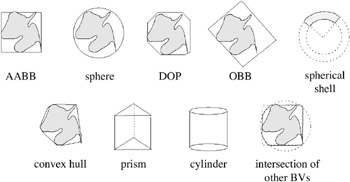
\includegraphics[height=6 cm, width = 6 cm, keepaspectratio = true]{bounding_volumes}
		\caption{Primjeri ograničavajućih volumena}
		\label{fig:1}
	\end{center}
\end{figure}

Kako je prikazano na Slici 2.1 postoji puno ograničavajućih volumena\cite{1}. U ovom radu biti će objašnjen AABB tj. Axis Aligned Bounding Box. Razlog tomu je AABB stablo koje se koristilo kasniej kao Bouning Volume Hierarchy, no o tome će biti riječi kasnije.

\section{AABB - Axis Aligned Bounding Box}

Kao što i samo ime govori, AABB je ograničavajući kvadrat koji je poravnat sa koordinatnim osima. Ovo je i ujedno najjednostavniji, ali i najbrži ograničavajući volumen\cite{1}.U 3D geometriji, kvadrat ima 6 stranica, a u 2D geometriji to je pravokutnik (sa 2 strane) \cite{1}. 
\begin{figure}[!http]
	\begin{center}
		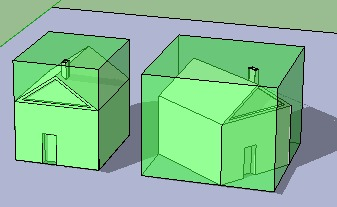
\includegraphics[height = 8 cm, width = 8 cm, keepaspectratio = true]{aabb}
		\caption{Axis Aligned Bounding Box prikazan zelenom bojom}
		\label{fig:2}
	\end{center}
\end{figure}

S obzirom da je AABB najjednostavniji oblik volumena, on nije uvijek točan. Ograničeni smo na korištenje pravokutnika pa iz toga slijedi da nećemo moći ograničiti objekt na onaj način na koji bismo željeli tj. postojati će neki "offset". U tom slučaju može se dogoditi da detektiramo sudar između objekata iako se on nije dogodio kao što je prikazano na slici.

\begin{figure}[!http]
	\begin{center}
		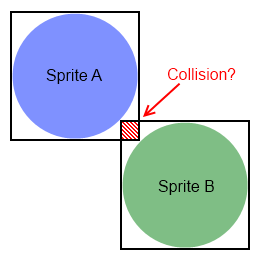
\includegraphics[height = 8 cm, width = 8 cm, keepaspectratio = true]{AABB_collision}
		\caption{Detektirani sudar između AABB-a koji se nije dogodio između objekata}
		\label{fig:2-1}
	\end{center}
\end{figure}

AABB u kodu možemo prikazati na nekoliko načina. Postoje 3 različite reprezentacije\cite{1} te ćemo u nastavku proći kroz sve te pobliže opisati opisati onu koja se koristila u ovome radu.

\subsection{Reprezentacije AABB-a}\label{sec::AABB_representation}

Prva i ona najčešća reprezentacija je reprezentacija koja koristi minimalnu i maksimalnu točku objekta.
Ukratko, pronađemo minimalnu i maksimalnu točku x,y i z koordinate te od tih točki napravimo kvadrat ako smo u 3D geometriji, tj. pravokutnik ako smo u 2D\cite{1}.

\begin{lstlisting}[style = {myC++},label ={code:1}, caption = {Struktura AABB-a koji koristi min i max točke}]
struct AABB{
	float min[3];
	float max[3];
}

\end{lstlisting}
\begin{figure}[!http]
 	\begin{center}
 		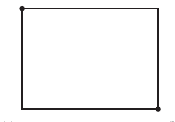
\includegraphics[height = 5 cm, width = 5 cm, keepaspectratio = true]{AABB_min-max}
 		\caption{AABB min-max reprezentacija u 2D geometriji}
 		\label{fig:3}
 	\end{center}
 \end{figure}
\newpage
Detektiranje sudara za ovu reprezentaciju je trivijalna. Provjerava se je li jedna koordinata minimalne točke jednog AABB-a veća od maksimalne koordinate točke drugog AABB-a ili obrnuto. Ukoliko to nije slučaj u sve 3 dimenzije, događa se sudar\cite{1}.

\begin{lstlisting}[style = {myC++},label={code:2}, caption = {Provjeravanje sudara za min-max reprezentaciju AABB-a\cite{1}}]
bool Collision(AABB a, AABB b)
{
	if (a.max[0] < b.min[0] || a.min[0] > b.max[0]) return 0;
	if (a.max[1] < b.min[1] || a.min[1] > b.max[1]) return 0;
	if (a.max[2] < b.min[2] || a.min[2] > b.max[2]) return 0;
	return 1;
}

\end{lstlisting}

Druga reprezentacija je korištenje minimalne točke i dijametra tj. udaljenosti do ostalih vrhova. Određivanje ovakvog volumena malo je kompliciranije nego u prethodnom slučaju upravo zbog dijametra koji moramo odrediti da bi ograničili objekt.

\begin{lstlisting}[style={myC++},label={code:3}, caption = {Struktura AABB-a koji koristi min točku i dijametar}]
struct AABB{
	float min[3];
	float dx,dy,dz; //udaljenost od minimalne tocke
}
\end{lstlisting}
 
 \begin{figure}[!http]
 	\begin{center}
 		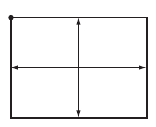
\includegraphics[height = 5 cm, width = 5 cm, keepaspectratio = true]{AABB_min-diametar}
 		\caption{AABB min-dijametar reprezentacija u 2D geometriji}
 		\label{fig:4}
 	\end{center}
 \end{figure}


Detekcija sudara za ovu reprezentaciju je također nešto kompliciranija nego u prethodnom slučaj i najmanje je "privlačna" od sve 3 reprezentacije \cite{1}.


\begin{lstlisting}[style = {myC++},label={code:4}, caption = {Provjeravanje sudara za min-width reprezentaciju AABB-a\cite{1}}]
bool Collision(AABB a, AABB b)
{
	float t;
	if ((t = a.min[0]- b.min[0]) > b.d[0] || -t > a.d[0]) return 0;
	if ((t = a.min[1]- b.min[1]) > b.d[1] || -t > a.d[1]) return 0;
	if ((t = a.min[2]- b.min[2]) > b.d[2] || -t > a.d[2]) return 0;
	return 1;
}
\end{lstlisting}

Posljednja reprezentacija, i ona koju smo koristili u radu, jest centar i radijus. Odredimo središnju točku našeg AABB-a i radijus u svim osima kojima izradimo AABB. Ova reprezentacija je najučinkovitija u terminima uštede memorije\cite{1}. 

\begin{lstlisting}[style = {myC++},label={code:5}, caption = {Struktura AABB-a koji koristi centar i radijus}]
struct AABB{
float center[3];
float rad[3]; //radijus
}
\end{lstlisting}

 \begin{figure}[!http]
 	\begin{center}
 		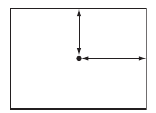
\includegraphics[height = 5 cm, width = 5 cm, keepaspectratio = true]{AABB_center-rad}
 		\caption{AABB centar-radijus reprezentacija u 2D geometriji}
 		\label{fig:5}
 	\end{center}
 \end{figure}
 \newpage
 Detektiranje sudara za ovu reprezentaciju je trivijalno. Za svaku dimenziju provjeravamo odnose centara i radijusa u svakoj dimenziji.
 
\begin{lstlisting}[style={myC++},label={code:6},caption={Provjeravanje sudara za centar-radijus reprezentaciju AABB-a\cite{1}}]
bool Collision(AABB a, AABB b)
{
	 if (Abs(a.c[0] - b.c[0]) > (a.r[0] + b.r[0])) return 0;
	 if (Abs(a.c[1] - b.c[1]) > (a.r[1] + b.r[1])) return 0;
	 if (Abs(a.c[2] - b.c[2]) > (a.r[2] + b.r[2])) return 0;
	 return 1;
}
\end{lstlisting}

Razlog biranja ove reprezentacije AABB-a leži u tome što smo odabrali kuglice kao objekte između kojih ćemo provjeravati sudar. S obzirom da je sfera, kao objekta, definirana centralnom točkom i radijusom, ova reprezentacija je odabrana kao najpogodnija.

\section{Kuglice}\label{sec:balls}

Kao što je već ranije spomenuto, objekti koji će se koristiti za detektiranje sudara u prostoru su kuglice tj. sfere. Kuglice su odabrane iz razloga što se vrlo jednostavno može odrediti fizikalna reakcija na sudar i što se na njih mogu lijepo primijeniti vanjske sile kao gravitacija i slično. Samim korištenjem kuglica i prijašnjim odabirom AABB-a kao ograničavajućih volumena javljaju se pojedini problemi.

Prvi i najveći problem u ovome slučaju je već spomenut. Naime, kako je to i prikazano na \ref{fig:2-1}, AABB ograniči prostor koji sfera ne pokriva tj. prostor koji je izvan sfere. To se može objasniti vrlo jednostavnom matematikom. Ako prikažemo stranicu kvadrata kao:
\begin{equation}
a = 2*r \label{eq:stranica}
\end{equation}
gdje nam je r radijus sfere tj. kuglice. Dalje, dijagonala kvadrata iznosi:
\begin{equation}
diag = a * \sqrt{2} \label{eq:dijagonala}
\end{equation}
može se zaključiti da je udaljenost od presjecišta dijagonala tj. centra kvadrata veća od radijusa sfere za $\sqrt{2}$. Što je veća sfera to je pogreška u ograničavajućem volumenu također veća. Zbog toga sigurno će se događati da ćemo otkrivati sudare i onda, kada se oni ne događaju, a pri vrlo velikim sferama to može stvarati puno nelogičnosti i čudnih fizikalnih reakcija na sudar.Kada su sfere vrlo malog radijusa, ta pogreška se u principu i ne primjeti, ali je ipak prisutna.

Na sreću ovome problemu se može uskočiti na vrlo dobar način. Naime, kako je prikazano na \ref{fig:1}, sfera sama po sebi može biti ograničavajući volumen \cite{1}. To proizlazi iz činjenice da se na vrlo jednostavan i elegantan način može detektirati sudar između 2 sfere. 

\begin{lstlisting}[style = {myC++},label={code:6-1}, caption = {Detekcija sudara između 2 sfere\cite{1}}]
bool SphereCollision(Sphere a, Sphere b)
{
// Calculate squared distance between centers
Vector d = a.c - b.c;
float dist2 = Dot(d, d);
// Spheres intersect if squared distance is less than squared sum of radii
float radiusSum = a.r + b.r;
return dist2 <= radiusSum * radiusSum;
}
\end{lstlisting}
U stvarnom kodu, implementacija ove funkcije izgleda nešto drugačije nego što je opisana ovdje i u literaturi, ali u principu algoritam i pristup su jednaki.
\newpage
\subsection{Implementacija klase za kuglice}

Implementacija klase za kuglice u principu je prilično jednostavna. Ona je prikazana sljedećim kodom:

\begin{lstlisting}[style = {myC++},label={code:7}, caption = {Implementacija klase za kuglice}]
public:
	Vector3D vecDir;
	AABB_box bBox;
	
	Ball() = default;
	Ball(const Point center, const float r, const float vecX, const float vecY,
		const float vecZ, const float m, const uint i);
	Ball(const float x, const float y, const float z, const float r,
		const float vecX, const float vecY, const float vecZ, const float m,
		const uint i);	
	void drawSphere();;
	void updatePosition(const float dt);
	bool collision(Ball &collider);
	template <typename T> bool collision(T &collider) {
		return isOverlap(this->bBox, collider.bBox);
	}
	void resolveCollision(Ball &collider);
	void resolveCollision(Wall &wall);
	Point &getCenter() { return this->center; }
	const float &x() const { return this->center.x; }
	const float &y() const { return this->center.y; }
	const float &z() const { return this->center.z; }
	const float &rad() const { return this->r; }
	const float &getMass() const { return this->mass; }
	const uint &getI() const { return this->i; }
private:
	Point center;
	float r;
	float mass;
	uint i;
};

\end{lstlisting}

U principu, da se primjetiti da se u samoj deklaraciji klase uglavnom nalaze konstruktori i get metode za dobivanje privatnih varijabli. Get i template metode su definirane u samoj deklaraciji klase zbog svoje jednostavnosti i veće brzine pristupanja.

U privatnim varijablama klase definirali smo najvažnije informacije o kuglici, a to su:

\begin{itemize}
	\item Center - točka centra za svaku kuglicu
	\item r - radijus sfere
	\item mass - masa sfere koja se kasnije koristi za količinu gibanja
	\item i - pozicija kuglice u listi kojom se osigurava da kuglica ne provjerava sudar sa samom sobom 

\end{itemize}

U javnim varijablama odredili smo:
\begin{itemize}
	\item bBox - odgovarajući AABB koji je opisan prethodno
	\newline
	U ovom slučaju bBox dobiva vrijednosti radijusa i centra od sfere kroz konstruktor
	\item vecDir - vektor definiran u klasi Vector3D koja sadrži osnovne operacije nad vektorima (skalarni produkt, oduzimanje, normaliziranje i sl.)
	\newline
	Ovaj objekt nam omogućava kretanje kuglice i olakšava izračunavanje sudara od zida i druge kuglice. Implementacija same klase biti će pokazana u kasnijim poglavljima.
	
\end{itemize}

Metode koje su definirane, u konačnosti govore same za sebe:
\begin{itemize}
	\item collision - detektira sudar kuglice ovisno o tipu s kojim se sudara.\newline
	Ukoliko se događa sudar sa drugom kuglicom, sudar se detektira na ranije opisani način. Sudar sa zidom i bilo kojim drugim objektom se detektira preko pridodanih AABB-a.
	\item resolveCollision - u metodama ovog imena definiramo fizikalnu reakciju kuglice na sudar. Ovisno o objektu s kojim se kuglica sudara, tako se i poziva određena resolveCollision funkcija
	\item drawSphere - funkcija za crtanje kuglica
	\newline
	Kuglice u prvom trenutku crtamo sa \emph{glutSolidSphere} i pomoću \emph{glTranslatef} ih pomičemo po prostoru. Kasnije, pri korištenju Opengl 3.3 kuglice će se crtati na drugačiji način.
	\item updatePosition - metoda kojom definiramo kretanje kuglica po prostoru uz pridodanu gravitaciju. \newline
	Detaljnija implementacija će biti kasnije objašnjena
\end{itemize}

U glavnom programu kuglice smo spremali u  \emph{std::vector}. Na taj način smo jednostavno iterativnim prolaženjem kroz listu iscrtavali kuglice, detektirali sudar između kuglica i zidova i u konačnosti pomicali kuglice po prostoru.
  
\chapter{Hijerarhija ograničavajućih volumena (eng. Bounding volume hierarchy)}\label{cha:BVH}
Prije nego što krenemo sa stvarnom animacijom i detekcijom sudara, trebali bi znati kako u stvarnome životu komplicirane objekte smjestiti u ograničavajući volumen. S obzirom da su objekti inače vrlo komplicirani, sastavljeni od puno različitih primitiva, potrebna nam je struktura podataka koja će na vjeran način ograničiti naš objekt. Ukoliko naš objekt ograničimo manjim volumenima i na pametan način te volumene posložimo u stablo, dobili smo određenu hijerarhiju volumena ili BVH. Možemo to prikazati na ovakav način:
\begin{itemize}
	\item Root element stabla ograniči cijeli objekt
	\item Njegova djeca ograniče lijevu i desnu polovicu objekta
	\item Djeca od ta 2 elementa podijele taj volumen na 2 dijela itd.
	\item Listovi sadrže ograničavajući volumen najmanjeg primitiva ili sami primitiv
\end{itemize}
Tako nešto možemo prikazati slikom.
\newpage
\begin{figure}[!http]
		\begin{center}
			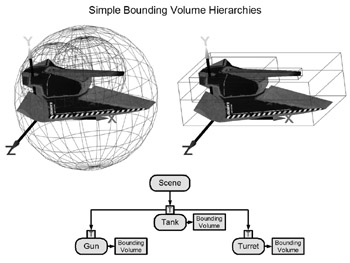
\includegraphics[height = 8 cm, width = 8 cm, keepaspectratio = true]{simple_bvh}
			\caption{Primjer BVH\cite{4}}
			\label{fig:6}
		\end{center}
\end{figure}
Konceptualno naš objekt bi prikazali na takav način. Ograničavajući volumen koji je roditelj u stablu, ograničuje druga 2 volumena i tako sve do listova koji su primitivi. Nešto kompleksnija struktura bila bi prikazana ovako:
\begin{figure}[!http]
	\begin{center}
		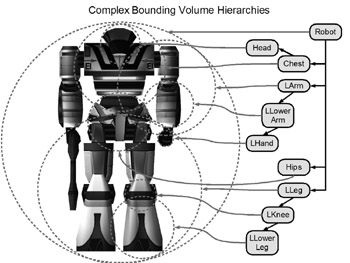
\includegraphics[height = 8 cm, width = 8 cm, keepaspectratio = true]{complex_bvh}
		\caption{Prikaz kompliciranije BVH \cite{4}}
		\label{fig:7}
	\end{center}
	\end{figure}
BVH možemo izgraditi od bilo kojih ograničavajućih volumena. U konačnici izgradnja samog stabla je uvijek proporcionalna broju elemenata od kojih je objekt sastavljen (složenost O(n))\cite{1}. Ono što je u ovom slučaju najbitnije je to da stablo ne moramo graditi u svakom frameu što nam prilično ubrzava posao. Također, važno je da stablo bude balansirano. Ukoliko je stablo dobro balansirano, objekt koji ograničavamo će biti točnije ograničen, nego što bi to bilo u nekom drugom slučaju. Za detektiranje sudara moramo samo provjeriti sudaraju li se u početku root elementi stabala. Ukoliko ne, odmah možemo izaći i prekinuti daljnju pretragu sudara, no sam algoritam i implementacija biti će prikazana kasnije.
	
Za potrebe ovog objekta odabrali smo AABB stablo zbog njegove efikasnosti i jednostavnosti prilikom implementacije. Kako je već i spomenuto, sudar između 2 AABB-a vrlo je jednostavno detektirati i to je glavna prednost ovoga stabla.

\section{AABB stablo}
S obzirom da smo rekli sve važno vezano za BVH, najbolje da uvod u AABB stablo napravimo s jednom slikom.
\begin{figure}[!http]
	\begin{center}
		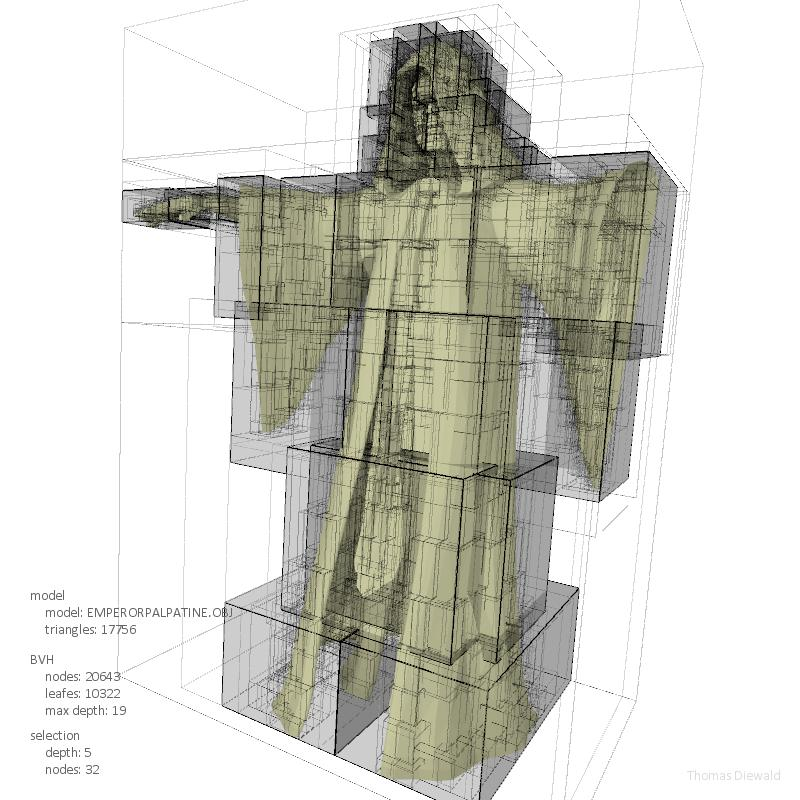
\includegraphics[height = 8 cm, width = 8 cm, keepaspectratio = true]{AABB_tree}
		\caption{Prikaz kompliciranog AABB stabla \cite{5}}
		\label{fig:8}
	\end{center}
\end{figure}
Ovakvo stablo izgleda prilično komplicirano. Ali, već i iz ovakvog kompliciranog objekta možemo vidjeti da se događaju nekakve pogreške. Te pogreške s jedno strane ipak nisu toliko bitne jer kada dođemo do djeteta toga elementa, primjetiti ćemo da se sudar ipak ne događa. Nešto jednostavniji primjer AABB stabla izgledao bi ovako:
\begin{figure}[!http]
	\begin{center}
		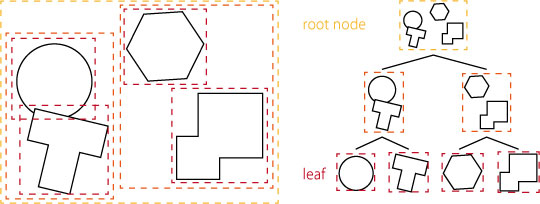
\includegraphics[height = 8 cm, width = 8 cm, keepaspectratio = true]{simple_aabb_tree}
		\caption{Prikaz jednostavnog AABB stabla}
		\label{fig:9}
	\end{center}
\end{figure}
\newline
Ovdje smo cijelu scenu podijelili AABB stablom, ali pristup je isti dijelimo li cijelu scenu ili jedan objekt. Scenu ćemo podijeliti ukoliko želimo provjeriti sudar zrake sa određenim objektom, a objekte ćemo podijeliti ukoliko želimo provjeriti sudar između samih objekata \cite{1}. 
\subsection{Ograničavanje 2 AABB minimalnim volumenom}\label{subsec:combineAABB}
Prije nego što se upustimo u izgradnju samog AABB stabla, potrebno je pronaći način kako 2 AABB ograničiti jednim većim volumenom. Uvjet je da je taj ograničavajući volumen minimalan za 2 AABB čiji ograničavajući volumen tražimo.

\begin{figure}[!http]
	\begin{center}
		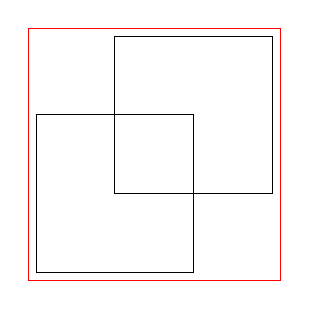
\begin{tikzpicture}
			\draw  (-2,-2) rectangle (0,0);
			\draw (-1,-1) rectangle (1,1);
			\draw[red] (-2.1,-2.1) rectangle (1.1,1.1);
		\end{tikzpicture}
		\label{fig:10}
		\caption{Minimalni ograničavajući volumen označen crvenom bojom}
	\end{center}
\end{figure}

Kako je to spomenuto ranije u \ref{sec::AABB_representation}, koristili smo reprezentaciju AABB-a sa točkom centra i radijusom. Pronalaženje ograničavajućeg volumena za ovakvu reprezentaciju AABB-a malo je zahtjevnije nego u slučaju sa min-max reprezentacijom.
\begin{algorithm}
\caption{Algoritam za izračunavanje minimalnog ograničavajućeg volumena za 2 AABB-a}
\label{alg:fatten_aabb}
\begin{algorithmic}
	\Function {getFattenAABB}{$AABB$ $a$, $AABB$ $b$}
		\State $AABB FattenAABB$ 
		\State$FattenAABB.r =\frac{distance(a.center,b.center)}{2}\ + Max(a.r,b.r)$
		\State$FattenAABB.center = median(a.center,b.center)$
		\State \Return $FattenAABB$
	
	\EndFunction
\end{algorithmic}
\end{algorithm}
\newline
Jednostavnom matematikom izračunamo udaljenost između 2 centra i pribrojimo joj veći od 2 radijusa (u našem slučaju radijusi su jednaki, ali zbog svih slučajeva stavljen je odabir maksimuma) da dobijemo radijus za naš AABB. Centar je jednostavno određen srednjom točkom između 2 centra od ulaznih AABB-a. Veći radijus odabran je iz razloga da s manjim nećemo moći ograničiti oba AABB-a i to zapravo neće biti ograničavajući volumen za 2 željena AABB-a. 
\subsection{Izgradnja AABB stabla}

Za izgradnju AABB stabla postoje 3 načina\cite{3}: 
\begin{itemize}
	\item Top down konstrukcija
	\item Bottom up konstrukcija
	\item Ubacivanje elemenata u stablo
\end{itemize}
Za sva 3 načina, potrebno je odabrati strategiju koja će napraviti što manje stablo. Ukoliko nam je stablo veliko pretraga elemenata u kojima se događa sudar će duže trajati. Zbog toga, potrebno je odabrati strategiju koja će stvoriti dobro balansirano ili približno dobro balansirano stablo\cite{1}. Ukoliko i ne stvorimo dobru strategiju za izgradnju stabla, uvijek možemo balansirati stablo "ručno" tj. putem funkcije. Ovo nikako nije poželjan slučaj. Time se gubi dodatno vrijeme na procesoru i funkcija za balansiranje je sama po sebi komplicirana i zahtjeva O(n) operacija. Za Top down i Bottom up konstrukciju potrebno je odabrati ravninu presijecanja (eng. Partitioning plane). Izgradnja ovoga stabla je u principu kao izgradnja svakog drugog stabla, samo je odabir ravnine presijecanja posao koji zahtjeva veliku količinu znanja i testiranja da u konačnici naše stablo bude minimalno. 
Ravnina presijecanja, kao što joj i samo ime govori, presjeći će listu naših objekata i pripadajućih AABB-a na onaj način kojim ćemo dobiti što manje stablo.Najjednostavniji model ravnine presijecanja je taj da se u listi elemenata odabere median element i da s obzirom na njegov AABB, izrađuje lijeva i desna grana stabla. Kao što je već rečeno, root element stabla će biti cijeli objekt te je potrebno samo odabrati pripadajuću točko centra i radijus (na ranije spomenuti način opisan u \ref{subsec:combineAABB} samo sa listom elemenata).

U ovom radu, odabrali smo treću strategiju za izgradnju stabla. Ubacivanje elemenata u prvom trenutku činilo se kao najlogičniji izbor jer je glavna ideja bila da se stablo elemenata izgrada prilikom sudara kuglica.

\begin{figure}[!http]
	\begin{center}

		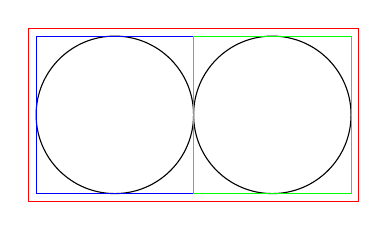
\begin{tikzpicture}
		\draw  (-1,0) circle (1);
		\draw (1,0) circle (1);
		\draw[blue] (-2,1) rectangle (0,-1);
		\draw[green] (0,-1) rectangle (2,1);
		\draw [red] (-2.1,1.1) rectangle (2.1,-1.1);
		\end{tikzpicture}
		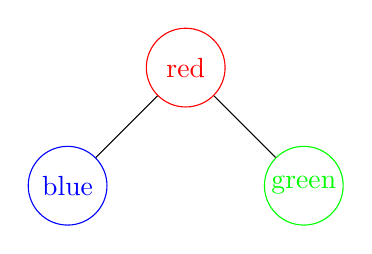
\begin{tikzpicture}[level distance=1.5cm,
		level 1/.style={sibling distance=3cm},
		level 2/.style={sibling distance=1.5cm}]
		\node[draw, circle,inner sep=1pt,minimum size = 1cm,red] {red}
		child {node[draw, circle,inner sep=1pt, minimum size = 1cm,blue] {blue}}
		child {node[draw, circle,inner sep=1pt,minimum size =1cm,green] {green}};
		\end{tikzpicture}		
	\end{center}
	\caption {Prikaz sudara 2 kuglice i pripadajućeg AABB stabla}
	\label{fig:11}
\end{figure}
Prema \ref{fig:11} stablo bi izgradili vrlo jednostavno. Nakon detekcije sudara, stvorili bi novi element, koji bi bio root element stabla (na \ref{fig:11} crvenom bojom). Njegov lijevi element pokazivao bi na lijevi AABB (plavom bojom), a desno dijete bi pokazivalo na desni AABB (zelenom bojom). 

Iako je primjer dosta trivijalan, još uvijek ne znamo kako nam klasa za AABB stablo izgleda, stoga još uvijek je sve prilično apstraktno. Klasa, kao i bilo koja druga klasa za stablo će sadržavati na lijevi i desni element stabla. To smo riješili pomoću "pametnih" pokazivača tj. u C++-u, \texttt{unique\char`_ptr}. Ovakav tip pokazivača nas rasterećuje brige o memoriji i njezinom brisanju. Osim toga, sadržimo "običan" pokazivač na element roditelja. Važan podatak koji nam također treba je i dubina stabla. Osim svega navedenog, ovakav tip stabla gradili smo u konstrukturu. Nema smisla stvarati AABB stablo od jedne kuglice, stoga je ovo bio zgodan način da se olakša sama implementacija algoritma za dodavanje dodatnih elemenata. Jednom kada bi izgradili stablo od 2 elementa, mogli smo dodati u njega bilo koji drugi element ubacivanjem na najbolju poziciju, tj. na poziciju gdje ćemo imati minimalno stablo.

\begin{lstlisting}[style=myC++, label = {code:8}, caption = {Implementacija klase za AABB stablo}]
class Node {
	typedef std::unique_ptr<Node> ptr;
	public:
		Node() = default;
		Node(const AABB_box bbox);
		Node(ptr &left, ptr &right);
	private:
		AABB_box box;
		ptr left;
		ptr right;
		Node *parent;
		int height;
};
\end{lstlisting}

Recimo da je bilo potrebno stvoriti iduću situaciju:

\begin{figure}[!htpb]
	\begin{center}
		
		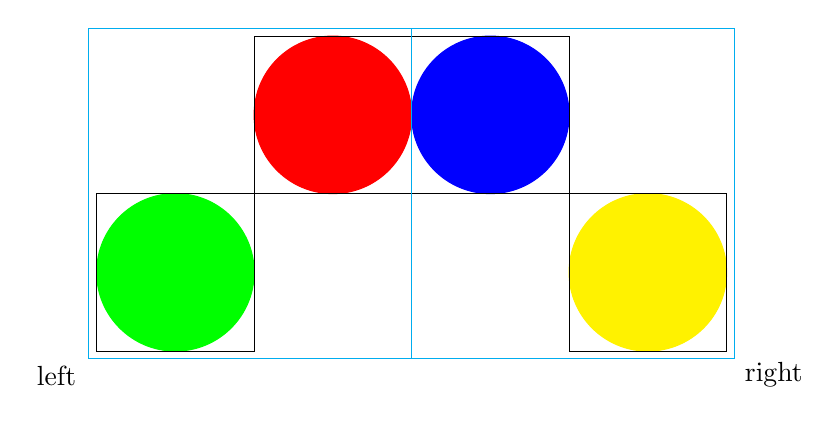
\begin{tikzpicture}
		\draw[red, fill = red]  (-1,0) circle (1);
		\draw[blue, fill = blue] (1,0) circle (1);
		\draw[green, fill = green] (-3,-2) circle (1);
		\draw[yellow, fill = yellow] (3,-2) circle (1);
		\draw (-2,1) rectangle (0,-1);
		\draw (2,1) rectangle (0,-1);
		\draw (-2,-1) rectangle (-4,-3);
		\draw (2,-1) rectangle (4,-3);
		\draw[cyan] (-4.1,-3.1) rectangle (4.1,1.1) node[black, pos = -.05] {left};
		\draw[cyan] (0,1.1) -- (0, -3.1) node[black, xshift = 4.6cm, yshift = -0.2cm] {right};
		\end{tikzpicture}
		\newline
	\end{center}
	\caption {Stablo od 4 kuglice}
	\label{fig:12}
\end{figure}
Prvo se sudare plava i crvena kuglica te se na taj način preko konstruktora izradi stablo sa 2 elementa. Nakon toga prvo udara žuta, a nakon toga zelena kuglica. Stablo koje ćemo dobiti izgledati će:
\newpage
\begin{figure}[!http]
	\begin{center}
		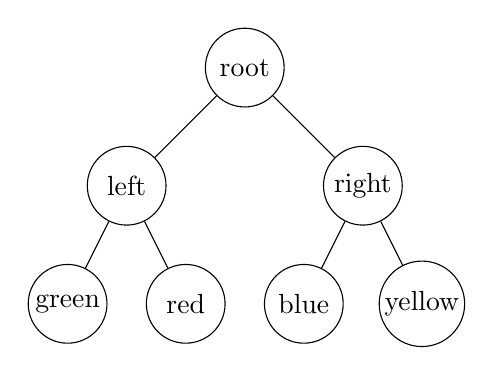
\begin{tikzpicture}[level distance=1.5cm,
		level 1/.style={sibling distance=3cm},
		level 2/.style={sibling distance=1.5cm}]
		\node[draw, circle,inner sep=1pt, minimum size = 1cm] {root}
		child {node[draw, circle,inner sep=1pt, minimum size = 1cm] {left}
			child {node[draw, circle,inner sep=1pt, minimum size = 1cm] {green}}
			child {node[draw, circle,inner sep=1pt, minimum size = 1cm] {red}}
		}
		child {node[draw, circle,inner sep=1pt, minimum size = 1cm] {right}
			child {node[draw, circle,inner sep=1pt, minimum size = 1cm] {blue}}
			child {node[draw, circle,inner sep=1pt, minimum size = 1cm] {yellow}}
		};

		\end{tikzpicture}
	\end{center}
	\caption {Prikaz AABB stabla za \ref{fig:12}}
	\label{fig:12-1}
\end{figure}
Nakon udara svake kuglice, ubacujemo novi AABB u naše stablo. Za to je korišten vrlo jednostavan algoritam. Primjećujemo da svaki element koji ubacujemo u stablo će biti list, stoga možemo slobodno reći da ova funkcija realizira ubacivanje lista u stablo\cite{6}. Prije samog algoritma, treba naglasiti da napisani algoritam možda nije najtočniji i možda ne radi za sve slučajeve. Algoritam je u svakom slučaju nedovoljno testiran, ali za ovako mali primjer poslužio nam je da vrlo dobro prikažemo strukturu AABB stabla. Algoritam radi na jednostavan način. Iteriramo po kreiranom stablu i izračunavamo površinu AABB-a od elementa koji želimo ubaciti i lijevog i desnog djeteta. Ukoliko je površina AABB-a od lijevog djeteta i elementa manja od površine AABB-a i desnog djeteta, iteriramo u lijevu stranu stabla. Ako je obrnuto, iteriramo na desnu stranu i tako sve dok ne dođemo do posljednjeg elementa stabla\cite{6}. S obzirom jesmo li išli lijevo ili desno, tu ubacujemo naš novokreirani element u stablo. U zadnjem koraku, vraćamo se od lista prema root elementu i radimo "update" AABB-a nad svakim elementom stabla.\newpage
\begin{algorithm}
	\caption{Algoritam za ubacivanje lista u AABB stablo}
	\label{alg:leaf_insertion}
	\begin{algorithmic}
		\Function {insertLeaf}{$AABBtree$ $node$, $AABB$ $box$}
		\While {$node$ is not leaf}
		\If{$Surface(node->left->box,box)>Surface(node->right->box,box)$}
		 \State $isLeft = false$
		\State $node = node->right$
		\Else
		\State $isLeft = true$
		\State $node = node->left$
		\EndIf
		\EndWhile
		\If{$isLeft is true$}
		\State $NewNode(box)$
		\State $FatAABB(node->parent->left, box)$
		\State $NewNode->parent = node->parent$
		\State $node->parent->left = NewNode$
		\Else
		\State $NewNode(box)$
		\State $FatAABB(node->parent->right, box)$
		\State $NewNode->parent = node->parent$
		\State $node->parent->right = NewNode$
		\EndIf
		\State Update tree until root with new leaf
		\EndFunction
	\end{algorithmic}
\end{algorithm}\newpage

\subsection{Pronalaženje sudara između dva stabla}
Nakon što smo izgradili naša stabla detektirati sudar između više njih nije nikakav problem. S obzirom da su stabla sagrađena od AABB-a potrebno je provjeriti samo root elemente, i ako se oni sudaraju idemo u daljnju elemenata stabala. Ukoliko sudara između root elemenata nije detektiran, sudar se nije ni dogodio. Ovakav način zahtjeva O(logN) operacija \cite{1}. Za jednostavan primjer možemo promotriti situaciju sa 2 jednostavna stabla koja imaju po 2 elementa. 

\begin{figure}[!http]	
	\begin{center}
		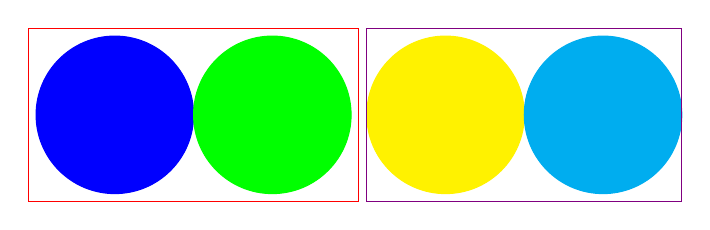
\begin{tikzpicture}
		\draw[fill = blue, blue] (-1,0) circle (1);
		\draw[fill = green, green] (1,0) circle (1);
		\draw[red] (-2.1,1.1) rectangle (2.1,-1.1);
		\draw[fill = yellow, yellow]  (3.2,0) circle (1);
		\draw[fill = cyan, cyan]  (5.2,0) circle (1);
		\draw [violet] (2.2,1.1) rectangle (6.2,-1.1);
		\end{tikzpicture}
	\end{center}
	\caption{Sudar između 2 jednostavna stabla}
	\label{fig:13}
\end{figure}
Za jedno i drugo stablo vrijedi struktura:
\begin{figure}[!http]	
	\begin{center}
		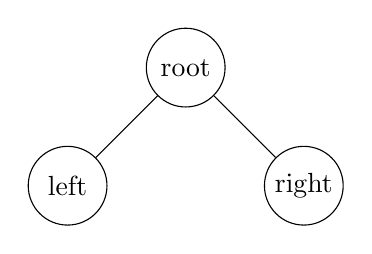
\begin{tikzpicture}[level distance=1.5cm,level 1/.style={sibling distance=3cm},level 2/.style={sibling distance=1.5cm}]
			\node[draw, circle,inner sep=1pt,minimum size = 1cm] {root}
				child {node[draw, circle,inner sep=1pt, minimum size = 1cm] {left}}
				child {node[draw, circle,inner sep=1pt,minimum size =1cm] {right}};
\end{tikzpicture}
	\end{center}
	\caption{Struktura stabla za \ref{fig:13}}
	\label{fig:13-1}
\end{figure}
U nekom trenutku, mi želimo točno znati da se dogodio sudar između zelene i žute kuglice (kuglice su prikazane drugom bojom samo radi razumjevanja). Na već opisani način detektiramo na kojem mjestu će se dogoditi sudar. Kada otkrijemo u kojem se listu dogodio sudar, taj sudar ćemo na neki određeni način riješiti i napraviti update na cijelom stablu. U našem slučaju kuglice su se odbile bez gubitka energije.\newpage
\begin{algorithm}
	\caption{Algoritam za detektciju sudara između 2 AABB stabla}
	\label{alg:search_collision}
	\begin{algorithmic}
		\Function {searchCollision}{$AABBtree$ $a$, $AABBtree$ $b$}
		\If{$isCollision(a,b)$ is false}
		\Return
		\EndIf
		\While{$a$ is not leaf}
		\If{$isCollision(a->left,b)$}
		\State $a = a->left$
		\Else 
		\State $a = a->right$
		\EndIf	
		\EndWhile
		\While{$b$ is not leaf}
		\If{$isCollision(b->left,a)$}
		\State $b = b->left$
		\Else 
		\State $b = b->right$
		\EndIf	
		\EndWhile
		\State $ResolveCollision(a,b)$
		\EndFunction
	\end{algorithmic}
\end{algorithm}\
Kao i \ref{alg:leaf_insertion}, ovaj algoritam također nije istestiran do kraja i vjerovatno u sebi ima neke pogreške, no za ovako jednostavne primjere će raditi. Ovime smo zapravo pokazali da nakon potpunog razumijevanja AABB stabla i strukture možemo vrlo jednostavno napisati kod za izgradnju stabla i detektiranje sudara između 2 ili više stabala.
\newpage

\section{Prednosti i mane BVH-a}
Glavna prednost BVH-a je brzina izgradnje stabala. Ovakvim jednostavnim algoritmima možemo izgraditi stablo i u njemu vrlo brzo provjeriti sudare. Ukoliko imamo puno manjih objekata koji se kreću po sceni, pretraga sudara je vrlo brza. Stablo ne moramo raditi u svakoj sekundi, nego ga je dovoljno izgraditi na početku i zatim samo tokom vremena raditi "update". Nažalost, u prvoj fazi izrade projekta, nije se smislila adekvatna strategija za detektiranje sudara pa je i samo korištenja BVH-a palo u vodu. 

Mana BVH-a je što se vrlo dobro mora razumjeti struktura s kojom se barata. Za razliku od algoritama koji particioniraju prostor i koji su intuitivniji za shvatiti, BVH zahtjeva od nas da dobro razumijemo algoritam i da na pametan način odaberemo os po kojoj ćemo podijeliti objekt ili scenu. 

Zaključno, BVH je struktura podataka kojom ćemo na vrlo jednostavan i jeftin način detektirati sudare na sceni ili među objektima. Uz malo više uloženog vremena, možemo napisati vrlo dobar algoritam koji će vrlo brzo detektirati sve sudare na sceni. Kako je i rečeno, od ovoga se odustalo. S vremenom nakon što je i sama struktura postala jasnija, donijele su se neke druge odluke vezane za sam rad i više nije imalo smisla koristiti i dalje implementirati BVH.

 	
	 % itd.
\chapter{Sudari, fizika i vanjske sile}
U ovom poglavlju, prije implementacije algoritma za podjelu prostora, prvo je potrebno opisati kakve će se uopće reakcije događati među kuglicama prilikom sudara. Potrebno je također i ograničiti našu scenu svojevrsnim zidovima. Vanjska sila je također važan dio ovoga projekta. Bilo je potrebno dodati gravitaciju na cijeloj sceni da se dobije dojam padanja kuglica i odbijanja od podloge. 

Prije početka samog rješavanja sudara među kuglicama potrebno je definirati i njihova kretanja. Kretanja su definirana u pomoćnoj klasi \emph{Vector3D}. Pomoću ove klase također su definirane normale zidova. Ovakav pristup znatno je olakšao samo rješavanje sudara jer se izjeglo korištenje kompliciranih trigonometrijskih jednadžbi i funkcija.\newpage

\section{Implementacija klase Vector 3D}\label{sec:vec3}

\begin{lstlisting}[style = myC++, label = {code:9}, caption={Implementacija klase Vector3D}]
class Vector3D {
public:
	Vector3D() = default;
	Vector3D(float x, float y, float z) {
		this->vec.emplace_back(x);
		this->vec.emplace_back(y);
		this->vec.emplace_back(z);
	}
	Vector3D(Point point) {
		this->vec.emplace_back(point.x);
		this->vec.emplace_back(point.y);
		this->vec.emplace_back(point.z);
	}
	Vector3D operator*(float const &scalar) {
		return Vector3D(this->x() * scalar, this->y() * scalar, this->z() * scalar);
	}
	Vector3D operator-(Vector3D &rhs) {
		return Vector3D(this->x() - rhs.x(), this->y() - rhs.y(),
		this->z() - rhs.z());
	}
	Vector3D normal() {
		float mag = std::sqrt(std::pow(this->x(), 2) + std::pow(this->y(), 2) +
		std::pow(this->z(), 2));
		if (mag == 0) {
			return Vector3D(1, 0, 0);
		}
		return Vector3D(this->x() / mag, this->y() / mag, this->z() / mag);
	}
	const float &x() const { return vec[0]; }
	const float &y() const { return vec[1]; }
	const float &z() const { return vec[2]; }
	void setX(const float &x) { vec[0] = x; 
	void setY(const float &y) { vec[1] = y; }
	void setZ(const float &z) { vec[2] = z; }

private:
	std::vector<float> vec;
};

inline float operator*(const Vector3D &lhs, const Vector3D &rhs) {
	return lhs.x() * rhs.x() + lhs.y() * rhs.y() + lhs.z() * rhs.z();
}

\end{lstlisting}
Ova klasa kako joj i samo ime govori, sadrži implementaciju najvažnijih vektorskih operacija:
\begin{itemize}
	\item Operator * će nam izračunati skalarni produkt između 2 vektora
	\item Funkcija normalize će normalizirati vektor
\end{itemize}
Naravno, za same vektore postoji još niz operacija, no ovdje su nam za sada bile potrebne samo ove dvije. Postavljene su i \emph{Set} metode za postavljanje vrijednosti u koordinate vektora. Ova klasa je header only i napisana je prema literaturi \cite{2}.

\section{Kretanje kuglica}
U ovom kratkom paragrafu objasniti ćemo kako se realiziralo kretanje kuglica po sceni. Kako je to objašnjeno u \ref{sec:balls}, za kretanje smo koristili funkciju pod imenom \emph{updatePosition} koja je za argument primala broj \emph{dt} što u prijevodu znači delta time ili razlika u vremenu između 2 framea. 
Brzinu kretanja kuglice definirali smo kao:
\begin{itemize}
	\item Brzina u X smjeru
	\item Brzina u Y smjeru
	\item Brzina u Z smjeru
\end{itemize}
Informacije o brzinama bile su spremljene u strukturi podataka \emph{Vector3D}, koju smo opisali u prethodnom paragrafu \ref{sec:vec3}. Kretanje kuglica definira se prema klasičnoj formuli iz mehanike:
\begin{equation}
		v = \frac{s}{t} \label{equ:brzina}
\end{equation}
gdje je:
\begin{itemize}
	\item v - brzina
	\item s - prijeđeni put
	\item t - vrijeme 
\end{itemize}
S obzirom da nama ne treba izračun brzine, nego nam je potreban put koji će kuglica prijeći u svakom trenutku, malom izmjenom i prilagodbom jednadžbe dobijemo:
\begin{equation}\label{equ:put}
\begin{aligned}
	s_x = vector.x * dt\\
	s_y = vector.y * dt\\
	s_z = vector.z * dt
	\end{aligned}
\end{equation}
gdje nam je:
\begin{itemize}
	\item vector.(x,y,z) - brzina u danoj koordinati
	\item s (x,y,z) - prijeđeni put u danoj koordinati
	\item dt - razlika vremena između 2 framea
\end{itemize}
Na ovakav jednostavan način dobili smo kretanje kuglice u bilo kojem smjeru, za sad bez nikakve vanjske sile tj. gravitacije.
\begin{figure}[!http]
	\begin{center}
		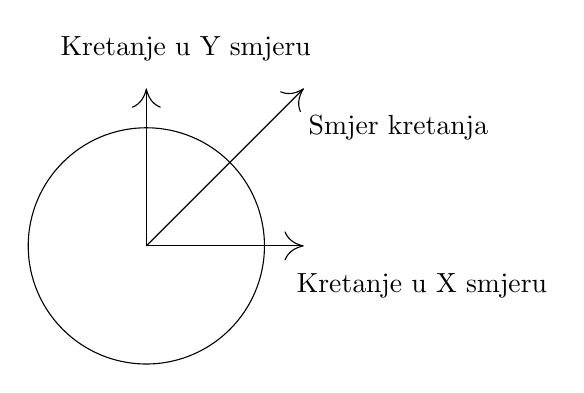
\begin{tikzpicture}
			\draw (0,0) circle (1.5);
			\draw[-{>[scale=3.5,length=2,width=3]},line width=0.4pt] (0,0) to (2,0) node[minimum size = 1pt, xshift = 1.5 cm, yshift = -0.5cm]{Kretanje u X smjeru};
			\draw[-{>[scale=3.5,length=2,width=3]},line width=0.4pt] (0,0) to (0,2) node[minimum size = 1pt, xshift = 0.5 cm, yshift = 0	.5cm]{Kretanje u Y smjeru};
			
			\draw[-{>[scale=3.5,length=2,width=3]},line width=0.4pt] (0,0) to (2,2) node[minimum size = 1pt, xshift = 1.2 cm, yshift = -0.5cm]{Smjer kretanja};
			
		\end{tikzpicture}
	\end{center}
	\caption {Kretanje kuglica realizirano jednostavnim zbrajanjem vektora}
	\label{fig:14}
\end{figure}

Sada kada nam je jasno definirano kretanje kuglica, potrebno je definirati kako će se kuglice ponašati prilikom sudara. S obzirom da su nam sve informacije spremljene u vektoru, to ne bi smjelo predstavljati nikakav problem. Korištenjem jednostavnih formula iz mehanike može se vrlo jednostavno dobiti reakcija kuglice na sudar sa drugom kuglicom ili zidom.

\section{Sudari kuglica}

Sudari su općenito mogu podijeliti u 2 skupine:
\begin{itemize}
	\item Neelastične sudare
	\item Elastične sudare
\end{itemize}
Neelastični sudari su oni sudari kod kojih se energija sustava gubi zbog različitih razloga (deformacija tijela u sudaru, toplina i sl.). Budući da u realnom sudaru najčešće dolazi djelomičnog gubitka energije, ima smisla ukazati i na tu problematiku\cite{9}. Analiza takvog sudara i dalje se temelji na zakonima očuvanja. Kod elastičnih sudara u zatvorenom sustavu nalaze se sva tijela masa m1 i m2 koja se gibaju brzinama v1 i v2 prije sudara, odnosno brzinama v'1 i v'2 poslije sudara\cite{9}.
\subsection{Sudari bez gubitka energije} \label{subsec:no_energy}
U prvom i najosnovnijem slučaju, razmotrili smo situaciju gdje nema nikakvog gubitka energije i gdje izlazne brzine nakon sudara ostaju jednake. Prva situacija je bila sljedeća.

\begin{figure}[!http]
	\begin{center}
		\begin{tikzpicture}
		\draw (-3,0) circle (1.5);
		\draw[-{>[scale=3.5,length=2,width=3]},line width=0.4pt] (-3,0) to (-1,0) node[minimum size = 1pt, xshift = -0.1 cm, yshift = 0.35cm]{v1};
		\draw (3,0) circle (1.5);
		\draw[-{>[scale=3.5,length=2,width=3]},line width=0.4pt] (3,0) to (1,0) node[minimum size = 1pt, xshift = -0.1 cm, yshift = 0.35cm]{v2};
		
		\end{tikzpicture}
	\end{center}
	\caption {Primjer sudara kuglica}
	\label{fig:15}
\end{figure}
Kuglice se kreću jedna prema drugoj, jedan se kreće brzinom v1, a druga brzinom v2. U trenutku sudara, kuglice će se odbiti jedna od druge i nastaviti se kretati brzinom v'1 tj. v'2.
\newpage
\begin{figure}[!http]
	\begin{center}
		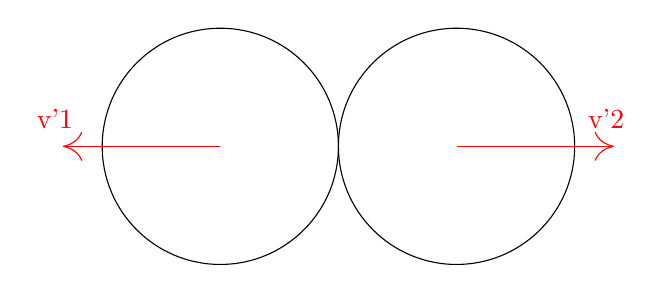
\begin{tikzpicture}
		\draw (-1.5,0) circle (1.5);
		\draw[-{>[scale=3.5,length=2,width=3]},line width=0.4pt,red] (-1.5,0) to (-3.5,0) node[minimum size = 1pt, xshift = -0.1 cm, yshift = 0.35cm]{v'1};
		\draw (1.5,0) circle (1.5);
		\draw[-{>[scale=3.5,length=2,width=3]},line width=0.4pt,red] (1.5,0) to (3.5,0) node[minimum size = 1pt, xshift = -0.1 cm, yshift = 0.35cm]{v'2};
		
		\end{tikzpicture}
	\end{center}
	\caption {Smjer gibanja kuglica nakon sudara}
	\label{fig:15-1}
\end{figure}
Nakon sudara vrijediti će sljedeće:
\begin{itemize}
	\item v'1 = -v1
	\item v'2 = -v2
 
\end{itemize}
Ovakav slučaj je trivijalan i nije problem odrediti smjer kretanja kuglica nakon sudara. Kretanje kuglica je samo u jednoj dimenziji te ukoliko pomnožimo brzinu kretanja kuglice sa (-1) dobiti ćemo rezultatnu brzinu nakon sudara.

Sljedeća situacija je kompliciranija. Kretanje jedne kuglice se događa u 2 dimenzije i to sada dodatno komplicira stvari. Situacija izgleda ovako:
\begin{figure}[!http]
	\begin{center}
		\begin{tikzpicture}
		\draw (-1.5,0) circle (1.5);
		\draw[-{>[scale=3.5,length=2,width=3]},line width=0.4pt] (-1.5,0) to (1,0) node[minimum size = 1pt, xshift = -0.1 cm, yshift = 0.35cm]{v1};
		\draw (3.5,-2) circle (1.5);
		\draw[-{>[scale=3.5,length=2,width=3]},line width=0.4pt] (3.5,-2) to (1.5,-0.5) node[minimum size = 1pt, xshift = 0.2 cm, yshift = -0.5cm]{v2};
		
		\end{tikzpicture}
	\end{center}
	\caption {Primjer sudara kuglica u 2 dimenzije}
	\label{fig:16}
\end{figure}
Primjetimo kako se druga kuglica, koja se giba brzinom v2, giba u 2 dimenzije (ima komponentu brzine u X smjeru i komponentu brzine u Y smjeru). Pretpostavimo da su mase kuglica jednake i da se pri njihovom sudare neće izgubiti nikakva energija. Rezultirajući vektori brzina više neće biti samo invertirani. Kuglica koja se giba samo po X osi (brzinom v1) nakon sudara dobiti će i neku svoju Y komponentu brzine.
\begin{figure}[!http]
	\begin{center}
		\begin{tikzpicture}
		\draw (-0.35,0) circle (1.5);
		\draw[-{>[scale=3.5,length=2,width=3]},line width=0.4pt,red] (-0.35,0) to (-2.5,1.5) node[minimum size = 1pt, xshift = -0.1 cm, yshift = 0.35cm,red]{v'1};
		\draw (2.5,-1) circle (1.5);
		\draw[-{>[scale=3.5,length=2,width=3]},line width=0.4pt,red] (2.5,-1) to (4.5,0.5) node[minimum size = 1pt, xshift = 0.2 cm, yshift = -0.5cm,red]{v'2};
		
		\end{tikzpicture}
	\end{center}
	\caption {Smjer gibanja kuglica nakon sudara u 2 dimenzije}
	\label{fig:17}
\end{figure}
Pretpostavimo da su i brzine kuglica u X smjeru jednake, pa će rezultat sudara približno jednak kao na \ref{fig:15}. Ovakav rezultat sudara možemo prikazati u nekoliko matematičkih koraka\cite{2}.

Prvo pronađemo vektor normale. To je vektor čije su komponente razlika između koordinata centara kuglica. Sukladno tome odmah pronađemo vektor tangente te oba vektora pomoću klase \emph{Vector3D} normaliziramo (kako je već i spomenuto pomoću ove klase puno nam je lakše pronaći vektor normale i tangente)\cite{2}.

\begin{figure}[!http]
	\begin{center}
		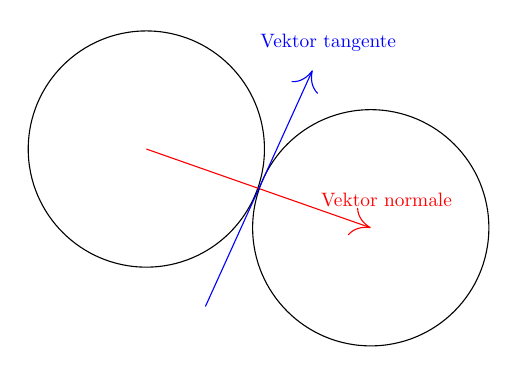
\begin{tikzpicture}
		\draw (-0.35,0) circle (1.5);
		\draw[-{>[scale=3.5,length=2,width=3]},line width=0.4pt,red] (-0.35,0) to (2.5,-1) node[minimum size = 1pt, xshift = 0.2 cm, yshift = 0.35cm,red, scale = 0.7]{Vektor normale};
		\draw (2.5,-1) circle (1.5);
		\draw[-{>[scale=3.5,length=2,width=3]},line width=0.4pt,blue] (0.4,-2) to (1.76,1) node[minimum size = 1pt, xshift = 0.2 cm, yshift = 0.35cm,blue, scale = 0.7]{Vektor tangente};

		\end{tikzpicture}
	\end{center}
	\caption {Vektor normale i tangente}
	\label{fig:18}
\end{figure}
Nakon toga, inicijalne brzine v1 i v2 pomnožimo sa jediničnim vektorima normale i tangente\cite{2}. Pomnožiti u ovome slučaju znači izračunati skalarni produkt između 2 vektora.
\begin{equation}\label{equ:dot_vector}
\begin{aligned}
		v'(1,2)n = un * v(1,2) \\
		v'(1,2)t = ut * v(1,2)
	\end{aligned}
\end{equation}
gdje nam je:
\begin{itemize}
	\item un - jedinični vektor vektora normale
	\item ut - jedinički vektor vektora tangente
	\item v (1,2) - vektori brzine kuglica
	\item v'n - rezultirajuća brzina u smjeru normale
	\item v't - rezultirajuća brzina u smjeru tangente
\end{itemize}
Tangencijalne brzine nakon sudara ostaju jednake što znači da smo u smjeru tangente izračunali brzinu\cite{2}. Nakon što smo odradili sve ove korake, pomoću jednostavne formule izračunamo rezultatne brzine za obje kuglice prema formuli:
\begin{equation}\label{equ:final_vec}
	\begin{aligned}
		v'1 = v'2n * un + v'1t * ut \\
		v'2 = v'1n * un + v'2t * ut
		\end{aligned}
\end{equation}
S ovim jendostavnim matematičkim koracima dobiti ćemo točno odbijanje kuglica nakon sudara kako je i prikazano na \ref{fig:17}. Ovo se može opisati i jednostavnim algoritmom koji je prikazan na idućoj strani.
\newpage
\begin{algorithm}
	\caption{Algoritam za izračunavanje smjera brzina nakon sudara između 2 kuglice}
	\label{alg:resolve_collision_1}
	\begin{algorithmic}
		\Function {resolveCollison}{$Ball$ $a$, $Ball$ $b$}
			\If {Collision($a ,b$) is false}
			\Return
			\EndIf
			\State $normal = (a.center - b.center)$
			\State $un = unitVector(normal)$
			\State $ut(-un.y,un.x)$
			\State $v1n = a.v * un$
			\State $v1t = a.v * ut$
			\State $v2n = b.v * un$
			\State $v2t = b.v * ut$
			\State $a.v = v1n * un + v1t * ut$
			\State $b.v = v2n * un + v1t * ut$
		\EndFunction
	\end{algorithmic}
\end{algorithm}\
Nakon pokretanja animacije primjećuje se jedan problem. Kuglice se slobodno gibaju po sceni i te u vrlo kratkom periodu izađu iz našeg viewporta. Našu scenu sada moramo ograničiti i to sa 4 strane s obzirom da još nismo implementirali gravitaciju. Za to će nam poslužiti klasa \emph{Wall} koju ćemo opisati u sljedećem poglavlju.

\subsection{Zidovi i klasa Wall}
Kako nam i samo ime govori, ova klasa služi za implementaciju granica tj. koji će ograničiti kretanje kuglica. Ove zidove nećemo vidjeti. Oni su nevidljivi i nalaze se na samim rubovima našeg prozora i ovise o \emph{lookAt} vektoru. Prvo bi bilo zgodno objasniti što i je taj \emph{lookAt} vektor. Laičkim rječnikom  možemo reći ovako: \emph{lookAt} vektor je vektor koji nam služi za pozicioniranje kamere na našoj sceni. Na primjer:\newpage
\begin{lstlisting}[style=myC++, label = {code:10}, caption={Primjer lookAt vektora iz glm knjižnice}]
glm::mat4 View = glm::lookAt(
	glm::vec3(0, 0, 50), // Camera is at (0,0,50), in World Space
	glm::vec3(0, 0, -1), // and looks at the origin
	glm::vec3(0, 1, 0)   // Head is up (set to 0,-1,0 to look upside-down)
	);
}
\end{lstlisting}
Prva linija govori nam gdje smo na našoj sceni postavili kameru. Prva linija dakle znači da se kameri nalazi na koordinatama (0,0,50) (udaljeni smo samo u Z smjeru). To znači da je naša X koordinata u rasponu od [-25, 25], a Y u rasponu od [-20,20] (razlog ovome je Aspect ratio koji je 4:3, no u ovome poglavlju to nije jako bitno).

Sada kada znamo konkretne koordinate našeg prozora, možemo proći kroz implementaciju same klase. Ona je u principu vrlo jednostavna, zidovi su zamišljeni kao obični AABB-i s kojima kuglice provjeravaju sudar. Kako je već spomenuto u \ref{sec:balls} kuglice imaju pridodjeljen odgovarajući AABB, pa te objekte možemo iskoristiti za detekciju sudara između zida i kuglice. Naravno i ovdje će se događati neke pogreške prilikom detekcije no to nam u principu nije jako bitno. Ovdje pogreška neće toliko utjecati na kretanje kuglice koliko bi u slučaju sudara između 2 kuglice. Zidovi također imaju pridodjeljen objekt klase \emph{Vector3D}, a u njemu nam je zapisana normala zida. Normala zida nam je vrlo bitna za izračun sudara kuglice i zida. Važno je naglasiti da je normala jedinični vektor.

\begin{figure}[!http]
	\begin{center}
		\begin{tikzpicture}
		\draw (-4,0) -- (4,0);
		\draw[-{>[scale=3.5,length=2,width=3]},line width=0.4pt,red] (0,0) to (0,2) node[minimum size = 1pt, xshift = 0.2 cm, yshift = 0.2cm,red, scale = 0.7]{Vektor normale};
		\end{tikzpicture}
	\end{center}
	\caption {Prikaz jednog zida i normale na zid}
	\label{fig:19}
\end{figure}
Zid ima AABB iste reprezentacije kao što imaju i kuglice, dakle radijus i centar. S obzirom na takvu reprezentaciju morali smo pažljivo izabrati koordinate centra i sam radijus. Vertikalni zidovi imali su Y koordinatu centra 0, a horizontalni zidovi su imali X koordinatu 0. Dalje, trebalo je odrediti radijus. Zidovi koji su vertikalni, imali su samo Y komponentu radijusa, dok su horizontalni imali samo X koordinatu radijusa. Primjer je u 2D, no logika i analogija je ista u sve 3 dimenzije. Samo bi dodali još 2 zida koji nam ograničavaju Z os i to je sve.
\begin{figure}[!http]
	\begin{center}
		\begin{tikzpicture}
		\draw[red] (-3,-2) rectangle (3,2);
		\tkzInit[xmax=4,ymax=4,xmin=-4,ymin=-4]
		\tkzAxeXY
		\end{tikzpicture}
	\end{center}
	\caption {Prikaz zidova u koordinatnom sustavu}
	\label{fig:20}
\end{figure}

Kada znamo sve ove informacije, implementacija same klase je prilično trivijalna. Ona je prikazana na idućoj strani.
\newpage
\begin{lstlisting}[style=myC++, label = {code:11}, caption={Implementacija klase Wall}]
class Wall {
public:
	AABB_box bBox;
	Vector3D vecDir;

	Wall() = default;
	Wall(const Point center, const float rX, const float rY, const float rZ,
		const float vecX, const float vecY, const float vecZ, const float m);
	Wall(const float x, const float y, const float z, const float rX,
		const float rY, const float rZ, const float vecX, const float vecY,
		const float vecZ, const float m);
	const float &x() const { return this->center.x; }
	const float &y() const { return this->center.y; }

	const float &z() const { return this->center.z; }
	const float &getMass() const { return this->mass; }
	Point &getCenter() { return this->center; }

private:
	Point center;
	float r[3];
	float mass;
	unsigned int i;
};

\end{lstlisting}
Primjećujemo da je implementacije klase u principu vrlo trivijalna. Nemamo nikakvih metoda, osim \emph{Get}, koje nam služe za dohvaćanje pojedinih privatnih varijabli. Među varijablama nalazi se i \emph{mass} što definira masu zida. Ovoj varijabli pridodali smo neku vrlo veliku vrijednost, i nju ćemo kasnije koristiti za elastične sudare između zida i kuglica. 
\subsection{Sudari kuglica i zida}
Nakon implementacije klase koje nam definiraju zidove, same sudare nije bio problem izračunati. U prvom trenutku ponovno nismo htjeli da se gubi energija kuglica. Sada će posebno do izražaja doći važnost normale zida. Htjeli smo da se kuglice odbije od zida pod istim kutom pod kojim se i sudarila. Ovakvim definiranjem normala, izbjegli smo korištenje trigonometrije i izračune upadnih i izlaznih kuteva.
\begin{figure}[!http]
	\begin{center}
		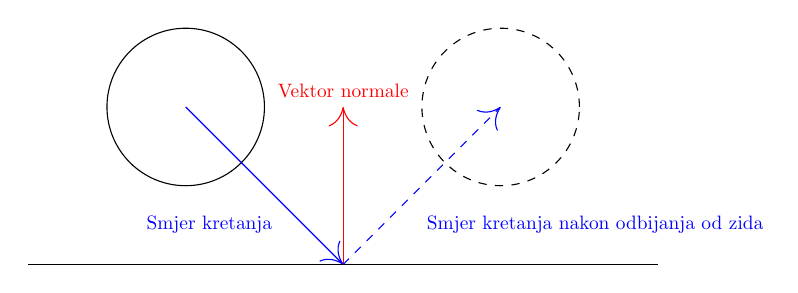
\begin{tikzpicture}
		\draw (-2,2) circle (1);
		\draw[-{>[scale=3.5,length=2,width=3]},line width=0.4pt,blue] (-2,2) to (0,0) node[minimum size = 1pt, xshift = -1.7 cm, yshift =0.5cm,blue, scale = 0.7]{Smjer kretanja};
		\draw (-4,0) -- (4,0);
		\draw[-{>[scale=3.5,length=2,width=3]},line width=0.4pt,red] (0,0) to (0,2) node[minimum size = 1pt, xshift = 0 cm, yshift = 0.2cm,red, scale = 0.7]{Vektor normale};
		\draw [dashed](2,2) circle (1);
		\draw[-{>[scale=3.5,length=2,width=3]},line width=0.4pt,blue,dashed] (0,0) to (2,2) node[minimum size = 1pt, xshift = 1.2cm,yshift =-1.5cm,blue, scale = 0.7]{Smjer kretanja nakon odbijanja od zida};
		\end{tikzpicture}
	\end{center}
	\caption {Reakcija kuglice na sudar sa zidom}
	\label{fig:21}
\end{figure}
Ovakav tip sudara možemo prikazati jednostavnom formulom:
\begin{equation}\label{equ:wall_collision}
		\begin{aligned}
			vector = vector - 2 * Dot(vector, normal) * normal;
		\end{aligned}
\end{equation}
gdje su:
\begin{itemize}
	\item vector - brzina i smjer kretanja kuglice
	\item normal - normala zida
	\item Dot - skalarni produkt
\end{itemize}
Ovo se također može prikazati jednostavni algoritmom koji je prikazan na sljedećoj stranici.\newpage
\begin{algorithm}
	\caption{Algoritam za izračunavanje smjera kretanja kuglice nakon sudara sa zidom}
	\label{alg:resolve_Wallcollision}
	\begin{algorithmic}
		\Function {resolveCollison}{$Ball$ $ball$, $Wall$ $wall$}
		\If {AABBCollision($ball ,wall$) is false}
		\Return
		\EndIf
		\State $DoubleDot = 2 * (ball.vector * wall.normal)$
		\State $collisionNormal = DoubleDot * wall.normal$
		\State $ball.vector = ball.vector - collisionNormal$
		\EndFunction
	\end{algorithmic}
\end{algorithm}

Sada naša animacija izgleda konačno kao nešto smisleno. Možemo dodati puno kuglica i testirati sudari između njih i sudare između kuglica i zidova. Prostor je ograničen i fizika odbijanja je smislena. Idući korak je dodavanje vanjske sile i gravitacije. Želimo da naše kuglice padaju, kao što je to situacija u stvarnome svijetu. Padanje i odbijanje od podloge. U sljedećem poglavlju razmotrit ćemo dodavanje gravitacije na kretanje kuglica i njihovo odbijanje od podloge. U konačnici, odbijanje od podloge će biti isto. No, nakon odbijanja s kuglicama se nešto treba dogoditi. Kuglice se u stvarnom svijetu ne mogu vječno odbijati od podloge. Mora se dogoditi gubitak kinematičke energije što će u nekom trenutku rezultirati da se kuglice prestanu gibati. Sve ove slučajeve razmotriti ćemo u narednim poglavljima.\newpage

\section{Sila teža} 
Sila teže je sila kojom Zemlja privlači neko tijelo mase m, označavamo ju najčešće slovom G. Ta sila privlači sva tijela prema središtu Zemlje pa je stoga tu i usmjerena.
Sila teže razlog je zbog kojeg sva bića i predmeti ne odlete u Svemir, već stoje na površini Zemlje.
Kada pustimo tijelo da slobodno pada s određene visine, ono se giba ubrzanjem g koje iznosi 9.81 $\frac{m}{s\textsuperscript{2}}$ neovisno o njegovoj težini što znači da će istovremeno pasti i iznimno teško i iznimno lagano tijelo ukoliko ih bacimo s iste visine.
No, na Mjesecu npr. ubrzanje kojim tijelo pada kada ga slobodno pustimo 6 je puta manje nego na Zemlji, tako da bi tamo ljudi lebdjeli iznad površine 
Nadalje, težina je posljedica djelovanja sile teže. To je sila kojom predmet djeluje na vodoravnu podlogu na koju je položen, npr. knjiga na stol, ili uteg na nit na koju je obješen.
Sila teža i težina jednake su po iznosu i smjeru djelovanja, ali nisu identični pojmovi.


\begin{figure}[!http]
	\begin{center}
		\begin{tikzpicture}
		\draw (0,3) circle (1);
		\draw[-{>[scale=3.5,length=2,width=3]},line width=0.4pt,red] (0,3) to (0,1) node[minimum size = 1pt, xshift = -1.7 cm, yshift =0.5cm,red, scale = 0.7]{Smjer djelovanja sile teže};
		\draw (-4,0) -- (4,0);

		\end{tikzpicture}
	\end{center}
	\caption {Djelovanje sile teže}
	\label{fig:22}
\end{figure}

Programski, ovo je vrlo jednostavno realizirati. S obzirom da je sila teža vertikalna sila, ona će djelovati samo na Y komponentu brzine kuglice. Opća formula sile teže glasi:
\begin{equation} \label{equ:sila_teza}
	\begin{aligned}
		G = m * g
	\end{aligned}
\end{equation}
gdje je:
\begin{itemize}
	\item m - masa objekta
	\item g - akceleracija sile teže koja iznosi 9.81 $\frac{m}{s\textsuperscript{2}}$
\end{itemize}
Ovo je samo formula sile i ona nam u ovom slučaju nije jako korisna. S obzirom da baratamo samo sa silama moramo iskoristiti drugu fizikalnu veličinu kojom ćemo regulirati brzinu da simuliramo silu težu. 

Fizikalna veličina koja nama zapravo treba je slobodni pad. Brzina slobodnog pada iznosi:
\begin{equation}\label{slobodni_pad}
	\begin{aligned}
		v = g * t
	\end{aligned}
\end{equation}
Slobodni pad je gibanje tijela isključivo pod utjecajem sile teže. Zakonitosti slobodnoga pada prvi je proučavao Galileo Galilei, te ustanovio da je prijeđeni put s proporcionalan kvadratu protekloga vremena t, a brzina v jednoliko raste s proteklim vremenom, te da gibanje ne ovisi o masi tijela koje pada \cite{10}.Uobičajeno je da se slobodni pad uzima kao primjer jednolikog ubrzanog gibanja (gibanja sa stalnim ubrzanjem). Pritom se pretpostavlja da nema otpora zraka ili trenja \cite{10}.

Sama implementacija slobodnog pada je trivijalna:
\begin{algorithm}
	\caption{Algoritam za implementaciju slobodnog pada}
	\label{alg:free_fall}
	\begin{algorithmic}
		\Function {updateBallPosition}{$Ball$ $ball$, $time$ $dt$}
		\State $ball.x += ball.vector.x * dt$
		\State $ball.y += ball.vector.y * dt - 9.81 * dt$
		\State $ball.z += ball.vector.z * dt$
		\EndFunction
	\end{algorithmic}
\end{algorithm}

U \ref{alg:free_fall} dt nam označava vrijeme koje je dobiveno između 2 framea. Na primjer, ukoliko imamo 60 sličica po sekundi, dt nam iznosi 16.6667 ms. Dobivanje razlike vremena između 2 framea je vrlo jednostavno. U nastavku ćemo prikazati implementaciju funkcije koja nam omogućuje izračunavanje proteklog vremena i kretanje kuglica po prostoru. \newpage
\begin{lstlisting}[style = myC++, label = {code:12}, caption = {Implementacije update funkcija}]

void Ball::updatePosition(float dt) {
double acc = -9.81;
this->vecDir.setY(this->vecDir.y() + acc * dt);
this->center.x += this->vecDir.x() * dt;
this->center.y += this->vecDir.y() * dt;
this->center.z += this->vecDir.z() * dt;
}

void update(int) {
nt = glutGet(GLUT_ELAPSED_TIME) / 1000.0f; //new time
dt = nt - ot; //delta time = new time - old time
ot = nt; //old time = new time

for (uint i = 0; i < balls.size(); i++) {
balls[i].updatePosition(dt);
}

glutPostRedisplay();
glutTimerFunc(16, update, 0);
}
\end{lstlisting}

Funkcija \emph{glutGet(\texttt{GLUT\_ELAPSED\_TIME})} će nam vratit broj milisekudni koje su prošle od \emph{glutInit} poziva (koji se stalno poziva na početku main petlje). Funkcija \emph{glutTimerFunc} će nam odrediti najmanji broj milisekundi koji će proći do idućeg poziva Update funkcije.

Stvari s gravitacijom gledane na ovakav način su zapravo dosta jasne. Na ovakav način možemo dodati bilo koju vanjsku silu koja će djelovati na kuglice. Iduće što želimo je da kuglice prilikom sudara izgube energiju. To će biti dodatno objašnjeno u idućem poglavlju.\newpage
\section{Elastični sudari}
U svim poglavljima do sada stalno se spominjala nekakva fizikalna reakcija kuglice na sudar. Svaka kuglica prilikom svog kretanja ima nekakvu kinetičku energiju. Opća formula kinetičke energije glasi:
\begin{equation}\label{equ:kinetic}
	\begin{aligned}
	E_{k} = \frac{m * v^2}{2}
	\end{aligned}
\end{equation}
gdje je:
\begin{itemize}
	\item m - masa kuglice 
	\item v - brzina kuglice
\end{itemize}
Prilikom sudara između 2 kuglice, dio kinetičke energije će se izgubiti, tj. prijeći će u iz jedne kuglice na drugu i obrnuto. S obzirom da vrijedi ZAKON OČUVANJA ENERGIJE, zbroj energije 2 kuglice se neće promijeniti. Zakon očuvanja energije nam govori da u u zatvorenom sustavu zbroj svih oblika energije (mehaničke, toplinske, električne, magneske i tako dalje) konstantan. Drugim riječima, u zatvorenom sustavu jedan oblik energije može prelaziti u druge oblike, a da se pri tom energija niti stvara niti poništava\cite{11}.

Iduća fizikalna pojava koju ćemo analizirati je količina gibanja. Količina gibanja ili zalet (oznaka p) je vektorska fizikalna veličina u klasičnoj mehanici koja opisuje gibanje čestice ili sustava čestica\cite{12}:
\begin{equation}\label{equ:impuls}
\begin{aligned}
	p = m * v
\end{aligned}
\end{equation}
gdje je:
\begin{itemize}
	\item m - masa čestice
	\item v - brzina čestice
\end{itemize}
Svaka kuglica koja se na sceni kreće, imati će količinu gibanja. Prilikom sudara količina gibanja količina gibanja jedne kuglice prenijeti će se na drugu kuglicu i obrnuto. Slično, kao i kod zakona o očuvanju energije, zakon očuvanja količine gibanja nam govori da količina gibanja izoliranog sustava je konstantna, odnosno, ukupna promjena količine gibanja u vremenu unutar izoliranog sustava jednaka je nuli\cite{12}.

Sada kada smo objasnili 2 važna fizikalna zakona, možemo definirati što je to elastični sudar zapravo. Kako smo i ranije rekli, elastični sudar je sudar tijela ulaze nekom brzinom v1 i v2, a izlazna brzina iz sudara im je v'1 i v'2. Kombinirajući zakon o očuvanju energije i zakon o očuvanju količine gibanja možemo reći slijedeće. Ukupna energija i ukupna količina gibanja prilikom sudara se ne mijenjaju, ali energija i količina gibanja određene kuglice se mijenja\cite{13}. Pokažimo to na jednom jednostavnom primjeru.
\begin{figure}[!http]
	\begin{center}
		\begin{tikzpicture}
		\draw (-3,0) circle (1.5) node[xshift = -1.5cm, yshift = 1.5cm]{m1};
		\draw[-{>[scale=3.5,length=2,width=3]},line width=0.4pt] (-3,0) to (-1,0) node[minimum size = 1pt, xshift = -0.1 cm, yshift = 0.35cm]{v1};
		\draw (3,0) circle (1) node[xshift = 1cm, yshift = 1cm]{m2};
		\draw[-{>[scale=3.5,length=2,width=3]},line width=0.4pt] (3,0) to (1,0) node[minimum size = 1pt, xshift = -0.1 cm, yshift = 0.35cm]{v2};
		
		\end{tikzpicture}
	\end{center}
	\caption {Primjer sudara kuglica različite mase i brzine}
	\label{fig:23}
\end{figure}
\newline
gdje je:
\begin{itemize}
	\item m1 \textgreater m2
	\item v2 \textgreater v1
\end{itemize}
S obzirom na mase i brzine možemo reći slijedeće. Kuglice će se nastaviti gibati u suprotnim smjerovima. Brzina v1 će se smanjiti s obzirom da je masa te kuglice veća. Brzina v2 će se povećati i kuglica će se kretati u suprotnom smjeru s većom brzinom.\newpage
\begin{figure}[!http]
	\begin{center}
		\begin{tikzpicture}
		\draw (-3,0) circle (1.5) node[xshift = -1.5cm, yshift = 1.5cm]{m1};
		\draw[-{>[scale=3.5,length=2,width=3]},line width=0.4pt,red] (-3,0) to (-5,0) node[minimum size = 1pt, xshift = -0.1 cm, yshift = 0.35cm,red]{v'1};
		\draw (3,0) circle (1) node[xshift = 1cm, yshift = 1cm]{m2};
		\draw[-{>[scale=3.5,length=2,width=3]},line width=0.4pt,red] (3,0) to (6,0) node[minimum size = 1pt, xshift = -0.1 cm, yshift = 0.35cm,red]{v'2};
		
		\end{tikzpicture}
	\end{center}
	\caption {Primjer sudara kuglica različite mase i brzine}
	\label{fig:24}
\end{figure} 
Iako su se brzine promijenile, ukupna količina gibanja ostala je jednaka. Sukladno tome vrijedi:
\begin{equation}\label{equ:kol_gib}
	m1 * v1 + m2 * v2 = m1 * v'1 + m2 * v'2
\end{equation}
Naravno, rekli smo da i ukupna količina energije ostaje jednaka, pa vrijedi:
\begin{equation}\label{equ:kol_energ}
\frac{1}{2} * (m1 * v1^2 + m2 * v2^2) = \frac{1}{2} * (m1 * v'1^2 + m2 * v'2^2)
\end{equation}
gdje su u obje jednadžbe:
\begin{itemize}
	\item m1, m2 - mase kuglica
	\item v1, v2 - brzine kuglica prije sudara
	\item v'1, v'2 - brzine kuglica nakon sudara
\end{itemize}
Nakon niza matematičkih operacija i skraćivanja izraza možemo donijeti konačne izraze koji će nam izračunati brzine kuglica nakon sudara. Oni glase\cite{13}:
\begin{equation}\label{equ:elastic_coll}
	\begin{aligned}
		v'1 = \frac{v1 * (m1 - m2) + 2 * m2 *v2}{m1 + m2}\\
		v'2 = \frac{v2 * (m2 - m1) + 2 * m1 *v1}{m1 + m2}
	\end{aligned}
\end{equation}
Ovi sudari vrijede samo za 1 dimenziju, ali to je u redu\cite{13}. Prema onome što smo ranije naveli u poglavlju \ref{subsec:no_energy} nama i trebaju samo 1D sudari. Objasnimo zašto. Ranije u \ref{subsec:no_energy} smo opisali jednadžbe kojima ćemo dobiti smjer kretanja kuglica nakon sudara bez gubitka količine energije i količine gibanja. U ovome poglavlju, objasnili smo kako će se ponašati samo vrijednosti brzina nakon sudara. Sve što mi trebamo sada napraviti je, ove 2 jednadžbe iz \ref{equ:elastic_coll} dodati u kod za rješavanje sudara kuglica. Prema \ref{alg:resolve_collision_1} možemo iznijeti slijedeći algoritam za to:\newpage
\begin{algorithm}
	\caption{Algoritam za izračunavanje smjera i iznosa brzina sudara između 2 kuglice uz promjenu količine gibanja jedne kuglice}
	\label{alg:resolve_collision_2}
	\begin{algorithmic}
		\Function {resolveCollison}{$Ball$ $a$, $Ball$ $b$}
		\If {Collision($a ,b$) is false}
		\Return
		\EndIf
		\State $normal = (a.center - b.center)$
		\State $un = unitVector(normal)$
		\State $ut(-un.y,un.x)$
		\State $v1n = a.v * un$
		\State $v1t = a.v * ut$
		\State $v2n = b.v * un$
		\State $v2t = b.v * ut$
		\State $v1(x,y,z) = \frac{v1n * (m1 - m2) + 2 * m2 *v2n}{m1 + m2}$
		\State $v2(x,y,z) = \frac{v2n * (m2 - m1) + 2 * m1 *v1n}{m1 + m2}$
		\State $a.v = v1 * un + v1t * ut$
		\State $b.v = v2 * un + v1t * ut$
		\EndFunction
	\end{algorithmic}
\end{algorithm}\

Ovime smo zaokružili cjelinu o kretanjima i sudaranjima kuglica. Ipak, problem je to što nam je sama detekcija sudara između svih kuglica prespora. Kako smo opisali ranije u poglavlju 2, postoje algoritmi za ubrzavanja same detekcije sudara. U narednim poglavljima cilj je opisati algoritam s kojim smo na zadovoljavajući način detektirali sve sudare na sceni i prema gore navedenim jednadžbama, iste sudare izračunali.


\chapter{Particioniranje prostora}
Kako je spomenuto u Uvodu, postoje razni algoritmi za detekciju sudara. Najvažniji od njih su oni kojima dijelimo objekte (BVH), i one kojima dijelimo prostor. Algoritam s kojim dijelimo objekt smo već prošlu u poglavlju \ref{cha:BVH}. Kako smo u nekom trenutku odustali od BVH-a bilo je potrebno pronaći dobar i brz način za detektiranje sudara na cijeloj sceni. Detekcija sudara sama po sebi, komplicirana je operacija i potrebno je da bude manje složena od O(n\texttt{$^2$}) operacija. Kako smo to opisali u poglavlju \ref{cha:BVH}, BVH-u je ptorebno O{logN} operacija sa detekciju sudara na sceni, iako je nekada prije potrebno napraviti dodatne kalkulacije i ažuriranja strukture da bi ona bila funkcionalna. To dodatno komplicira stvari, ali je vrlo efikasno. U ovom poglavlju, pokazati ćemo da je particioniranje prostora također jedna efikasna i lako razumljiva strategija za detekciju sudara.

\section{Primitivna detekcija sudara}
U prošlom poglavlju objašnjeno je kako sudare, nakon što ih detektiramo, kalkulirati. Nigdje nismo spomenuli kako smo i te sudare detektirali. Koristili smo za to vrlo primitivan i jednostavan algoritam. Za svaki objekt na sceni, iterativno bi tražili s kojim se objektom sudara. Ovo u principu nije problem kada je situacija sa zidovima jer u konačnici imamo 4 zida pa je sama složenost te operacije O(4 * N). Problem se javlja kada imamo kuglica. Do 50 kuglica ovaj algoritam će raditi, no nakon prelaska na veći broj kuglica javlja se problem. Za 500 kuglica potrebno je napraviti isto toliko provjera. To nas dovodi do brojke od 250 000 tisuća provjera i složenosti O(n\texttt{$^2$}). Kako smo ranije opisali ovo smo željeli izbjeći. Takav algoritam bi glasio ovako:
\begin{algorithm}
	\caption{Algoritam za primitivnu detekciju sudara između kuglica}
	\label{alg:primitive_collision}
	\begin{algorithmic}
		\Function {searchCollisions}{$Ball$ $list[N]$}
		\State $i = 1$
		\For {$ball$ in $list$}
		\While{$i < N$}
		\If {$ifCollision(ball, list[i])$}
		\State $resolveCollision(ball,list[i])$
		\EndIf
		\State $i++$
		\EndWhile
		\EndFor
		\EndFunction
	\end{algorithmic}
\end{algorithm}
gdje je:
\begin{itemize}
	\item list - lista kuglica
	\item N - broj kuglica
\end{itemize}
Kako je već spomenuto, za listu smo koristili \emph{std::vector} u C++. Ovakav pristup smo koristili samo pri početku projekta. Za mali broj kuglica i za provjeru ispravnosti proračuna, ovakav pristup je bio dovoljan. \newpage
\section{k-dimenzionalno stablo (K-dimensional tree - k-d)}
Složenost koju želimo postići pri detektiranju sudara najmanje O(NlogN) (za N objekata na sceni). Da bi to postigli prostor se mora podijeliti u smislene regije u kojima ćemo provjeravati sudar. Promotrimo to na jednom primjeru:
\begin{figure}[!http]	
	\begin{center}
		\begin{tikzpicture}
		\draw (0,-2) rectangle (10,10);
		\draw (5,4) circle(0.7) node {1};
		\draw (9,6) circle(0.7) node {3};
		\draw (4,7) circle(0.7) node{2};
		\draw (8,1) circle(0.7) node {5};
		\draw (7,2) circle(0.7) node {4};
		\draw (2,3) circle(0.7) node {6};
		\end{tikzpicture}
	\end{center}
	\caption{Primjer kuglica na sceni}
	\label{fig:26}
\end{figure}\newline
gdje su koordinate centara:\newpage
\begin{itemize}
	\item 1 - (5,4)
	\item 2 - (4,7)
	\item 3 - (9,6)
	\item 4 - (7,2)
	\item 5 - (8,1)
	\item 6 - (2,3)
\end{itemize}
Na slici \ref{fig:25} vidimo da ne treba u svim situacijama provjeravati sudar. Na primjer za kuglicu 2 i 6 znamo da se sudar neće dogoditi te tu provjeri ne moramo uzimati u obzir dok između kuglica 5 i 4 te 1 i 2 znamo da bi se mogao dogoditi sudar u skorom vremenu, te, te sudare moramo provjeriti.

Postoje mnoge tehnike za podijeliti prostor, no ona koju smo mi koristili je k-d stablo. K-d stablo je binarno stablo gdje je svaki čvor k-dimenzionalna točka\cite{14}. Svaki čvor koji nije list, može se shvatit kao ravnina koja dijeli prostor. Točke koje se nalaze lijevo od ravnine predstavlja lijeva strana stabla, dok desne točke predstavlja desna strana stabla\cite{14}. Konkretno, ukoliko odaberemo X os za os podijele, točke manje od vrijednosti X bit će nam u lijevoj grani stabla, dok točke veće od X vrijednosti će biti na desnoj strani stabla\cite{14}. U 3D prostoru intuitivno je da ćemo imat 3 dimenzije. Dakle, root čvor stabla će podijeliti prostor prema X koordinati, zatim njegova djeca prema Y koordinati, djeca djece po Z koordinati itd. .
\begin{figure}[!http]
	\begin{center}
		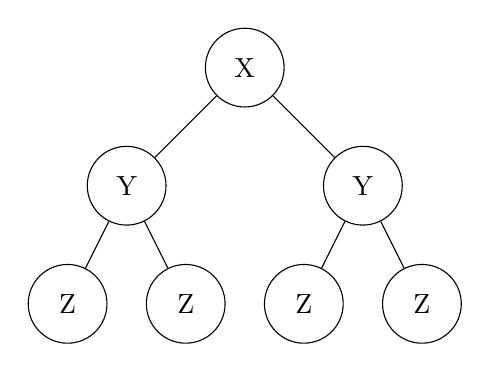
\begin{tikzpicture}[level distance=1.5cm,
		level 1/.style={sibling distance=3cm},
		level 2/.style={sibling distance=1.5cm}]
		\node[draw, circle,inner sep=1pt, minimum size = 1cm] {X}
		child {node[draw, circle,inner sep=1pt, minimum size = 1cm] {Y}
			child {node[draw, circle,inner sep=1pt, minimum size = 1cm] {Z}}
			child {node[draw, circle,inner sep=1pt, minimum size = 1cm] {Z}}
		}
		child {node[draw, circle,inner sep=1pt, minimum size = 1cm] {Y}
			child {node[draw, circle,inner sep=1pt, minimum size = 1cm] {Z}}
			child {node[draw, circle,inner sep=1pt, minimum size = 1cm] {Z}}
		};
		
		\end{tikzpicture}
	\end{center}
	\caption {Prikaz k-d stabla za 3 dimenzije}
	\label{fig:25}
\end{figure} \newline
Nakon što smo došli do Z dimenzije, ponovno dijelimo prostor po $x$ koordinati, i tako se vrtimo dok ne podijelimo cijeli prostor. 
Sada se možemo vratiti na situaciju iz slike \ref{fig:26}. k-d stablo će nam onakav prostor podijeliti na sljedeći način\cite{14}:
\begin{figure}[!http]
	\begin{center}
		\begin{tikzpicture}
		\draw (0,0) rectangle (10,10);
		\draw (5,4) circle(0.7) node {1};
		\draw[blue] (0,4) -- (7,4);
		\draw (9,6) circle(0.7) node {3};
		\draw[blue] (7,6) -- (10,6);
		\draw (4,7) circle(0.7) node{2};
		\draw[red] (4,4) -- (4,10);
		\draw (8,1) circle(0.7) node {5};
		\draw[red] (8,0) -- (8,6);
		\draw (7,2) circle(0.7) node {4};
		\draw[red] (7,0) -- (7,10);
		\draw (2,3) circle(0.7) node {6};
		\draw[red] (2,0) -- (2,4);
		\tkzInit[xmax=10,ymax=10,xmin=-2,ymin=-2]
		\tkzAxeXY

		\end{tikzpicture}
	\end{center}
	\caption {Podjela prostora k-d stablom}
	\label{fig:27}
\end{figure}\newline
Primjetimo da smo prostor podijelili po koordinatama centra svake kuglice.Crvene linije prikazuju podjelu prostora po X koordinati, dok plave ukazuju na podjelu prostora po Y koordinati. Da smo imali još Z koordinatu, analogija je ista, imali bi dodatnu dimenziju, no zbog jednostavnosti dovoljno je ovo prikazati u 2D prostoru.\newpage

\subsection{Izgradnja k-d stabla}
U prijašnjem poglavlju podijelili smo prostor bez da znamo zapravo kako je to napravljeno, niti da znamo kako će struktura stabla izgledati za takvu situaciju. Općenito, znamo kako struktura stabla izgleda. Svaka razina stabla particionirala je prostor po nekoj koordinati. Jedino pitanje koje se postavlja je, kako izabrati točke na način da dobijemo kvalitetno podijeljen prostor i balansirano stablo. S obzirom da postoji puno načina na koji možemo odabrati osi presijecenja koje su poravnate s koordinatnim osima, postoji i puno načina da izgradimo k-d stablo. Kanonski način izgradnje je onaj koji smo već opisali\cite{14}:
\begin{itemize}
	\item Kako se krećemo po stablu, kružno biramo osi presijecanja
	\item Točke odabiremo tako da odaberemo median element s obzirom na os presijecanja
\end{itemize}
Ovakva metoda će nas dovesti do balansiranog stabla, iako za sve aplikacije to nije nužan uvjet \cite{14}.

S obzirom na sve ovo možemo napisati jednostavan algoritam za izgradnju samog k-d stabla.

\begin{algorithm}
	\caption{Algoritam za izgradnju k-d stabla\cite{14}}
	\label{alg:k-d_tree_build}
	\begin{algorithmic}
		\Function {K-d tree}{$Point$ $pointList[N]$, $depth$}
		\State $axis = depth\mod{k}$ 
		\State $Sort(list)$
		\State Select $median$ by $axis$ from $pointList$
		\State $Node.point = median$
		\State $Node.left(pointList[0...Median-1], depth+1)$
		\State $Node.right(pointList[Median+1...pointList.size], depth+1)$
		\EndFunction
	\end{algorithmic}
\end{algorithm}
\newpage
Sada kada znamo izgraditi stablo možemo prikazati kako bi stablo konkretno izgledalo za situaciju na slici \ref{fig:27} it prošlog poglavlja:
\begin{figure}[!http]
	\begin{center}
		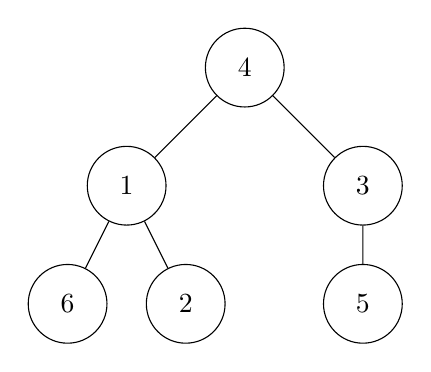
\begin{tikzpicture}[level distance=1.5cm,
		level 1/.style={sibling distance=3cm},
		level 2/.style={sibling distance=1.5cm}]
		\node[draw, circle,inner sep=1pt, minimum size = 1cm] {4}
		child {node[draw, circle,inner sep=1pt, minimum size = 1cm] {1}
			child {node[draw, circle,inner sep=1pt, minimum size = 1cm] {6}}
			child {node[draw, circle,inner sep=1pt, minimum size = 1cm] {2}}
		}
		child {node[draw, circle,inner sep=1pt, minimum size = 1cm] {3}
			child {node[draw, circle,inner sep=1pt, minimum size = 1cm] {5}}
		};
		
		\end{tikzpicture}
	\end{center}
	\caption {Prikaz strukture k-d stabla za sliku \ref{fig:27}}
	\label{fig:28}
\end{figure}
Prikažimo ovo isto stablo sa koordinatama centara\cite{14}:
\begin{figure}[!http]
	\begin{center}
		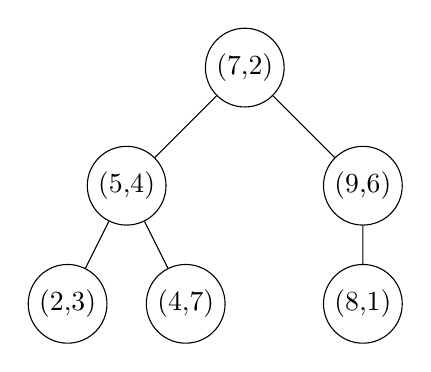
\begin{tikzpicture}[level distance=1.5cm,
		level 1/.style={sibling distance=3cm},
		level 2/.style={sibling distance=1.5cm}]
		\node[draw, circle,inner sep=1pt, minimum size = 1cm] {(7,2)}
		child {node[draw, circle,inner sep=1pt, minimum size = 1cm] {(5,4)}
			child {node[draw, circle,inner sep=1pt, minimum size = 1cm] {(2,3)}}
			child {node[draw, circle,inner sep=1pt, minimum size = 1cm] {(4,7)}}
		}
		child {node[draw, circle,inner sep=1pt, minimum size = 1cm] {(9,6)}
			child {node[draw, circle,inner sep=1pt, minimum size = 1cm] {(8,1)}}
		};
		
		\end{tikzpicture}
	\end{center}
	\caption {Prikaz strukture k-d stabla za sliku \ref{fig:27}}
	\label{fig:28-1}
\end{figure}

Složenost ovog algoritma ovisi o složenosti operacije sortiranja i pretrage za median elementom. Pozicija median elementa se pronalazi kao:
\begin{equation}
	Median =\frac{N}{2}
\end{equation}
gdje je:
\begin{itemize}
	\item N - broj elemenata
\end{itemize}
Algoritmi koji se uglavnom koriste za sortiranje su \emph{Mergesort} (implementiran u C++ STL-u) i \emph{Heapsort}. Složenost ovih algoritama u općem slučaju je O(NlogN). Sukladno tome to je i najbolja složenost koja se može postići s ovim algoritmima sortiranja. Složenost izgradnje stabla u najgorem slučaju može biti O(kNlogN) operacija što ćemo mi i imati s obzirom da u svakoj od k dimenzija moramo sortirati točke i odabrati median element. S obzirom da se kuglice na sceni kreću, stablo moramo graditi u svakom frameu pa je i ovakav način detekcije sudara sam po sebi dosta složen, no još uvijek je brži od onog opisanog u algoritmu \ref{alg:primitive_collision}. 

Sada je potrebno pretražiti sve potencijalne sudare na sceni. Dobra osobina k-d stabla je ta što će nam podijeliti prostor po gustoći točaka. Tako možemo vrlo jednostavno detektirati sudare na sceni i izračunati ih ukoliko se sudar dogodio.

\subsection{Pretraga sudara u k-d stablu}
Pretraga sudara u k-d stablu nakon izgradnje je trivijalna stvar. Sve se svodi na jednostavno "šetanje" po stablu. Da dodatno ne povećavamo složenost, šetanje će uključiti samo onu granu stabla koja je bliže u prostoru i/ili onu s kojom se kuglica sudara. Da se izbjegne korištenje funkcije korijena (\emph{sqrt}) koristiti će se kvadrirana udaljenost (eng. \emph{squared distance}). Ukoliko detektiramo sudar, u istom trenutku ga i računamo. Algoritam je rekurzivan i glasi:\newpage
\begin{algorithm}
	\caption{Algoritam za pretragu sudara u k-d stablu}
	\label{alg:serch_collisions_kd}
	\begin{algorithmic}	
		\Function {searchCollisions}{$Ball ball$, $K-dTreeNode Node$}
		\If {$Node$ is leaf}
		\If {$isCollision(ball, node)$}
		\State $resolveCollision(ball,node)$
		\EndIf
		\Return
		\EndIf
		\If {$isCollision(ball, node)$}
			$resolveCollision(ball,node)$
		\EndIf
		\If{$distance(Node.left,ball) > distance(Node.right,ball)$ or
		\State $isCollision(ball, node.right)$}
		\State $searchCollisions(ball, node.right)$
		\ElsIf{$distance(Node.right,ball) > distance(Node.left,ball)$ or \State $isCollision(ball, node.left)$}
		\State $searchCollisions(ball, node.left)$
		\EndIf
		\EndFunction
		
		\Function {checkAllBalls}{$Ball listBall[N]$, $K-dTreeNode Node$}
		\For {$ball$ in $listBall$}
		\State $searchCollisions(ball,Node)$
		\EndFor
		\EndFunction

	\end{algorithmic}
\end{algorithm}
Na ovakav ćemo način jednostavno na cijeloj sceni detektirati sudare i izračunati. S obzirom da je kuglica uvijek u sudaru sama sa sobom, potrebno je izbjeći računanje takvog sudara. Prilikom implementacije klase za kuglice, u kodu \ref{code:7}, spomenuli smo atribut \emph{i} tipa integer. Ovaj atribut označava poziciju kuglice u listi i na taj način ćemo vrlo jednostavno izbjeći računanje sudara kuglice same sa sobom. Testiranjem je utvrđeno da se prilikom takvog računanja mogu pojaviti anomalije i ponašanje kuglica koje ne želimo.\newpage
\subsection{Implementacija klase za k-d stablo}
U ovome poglavlju nećemo prikazivati implementaciju svih funkcija. Opisati ćemo samo odluke i strukturu same klase.
\begin{lstlisting}[style = myC++, label = {code:13}, caption={Implementacija klase za k-d stablo}]

template <class T> class KDtreeNode {
static bool sortbyX(T lhs, T rhs) 
static bool sortbyY(T lhs, T rhs) 
static bool sortbyZ(T lhs, T rhs) 

public:
	KDtreeNode *left()
	KDtreeNode *right() 
	unsigned long childSize() 
	unsigned int getPlane()
	void build_tree(std::vector<T> &v, int depth) 
	void treeTraverse() 
	template <class T1> void searchCollisions(T1 &ball)
private:
	std::vector<KDtreeNode> child;
	T object;
	unsigned int plane;
};

\end{lstlisting}

U početku bila je dilema koristiti li normalnu klasu koja bi radila samo na temelju kuglica, ili \emph{template} klasu koja bi onda radila za sve tipove objekata koje bi stavili scenu. Odabrana je \emph{template} klasa upravo iz tog razloga, da prilikom dodavanja nekih drugih objekata koji nisu kuglice, ne moramo raditi novu strukturu za samo taj specifični objekt. Točnost ove tvrdnje pokazana je kada se ista klasa za k-d stablo koristila i za particioniranje zidova. Jednom strukturom smo odradili posao za sve moguće objekte na sceni. Postoji i bolji pristup da se koriste samo točke objekata, ali za nas je ovakav bio dovoljan. Klase \emph{sortby(x,y,z)} poslužile su za sortiranje cijele liste prema određenoj osi. Ostale funkcije koje smo koristili su ili već opisane (\emph{build\texttt{\_}tree}, \emph{searchCollisions}) ili su samo \emph{Get} funkcije za dohvat privatnih varijabli. \newpage
\section{Prednosti i mane korištenja algoritama za particioniranje prostora (k-d stabla)}

K-d stablo svakako pronalazi svoju uporabu u stvarnome svijetu. Vrlo jednostavna implementacija i razumijevanje same strukture omogućuje široku primjenu u svijetu igara. Skladno tome, jasno je da je k-d stablo dobar način kojim ćemo pretraživati sudare na sceni. Vrlo je efikasno iako ima svoje mane. 

Prva od njih je ta da u svakom koraku izgradnje stabla moramo sortirati cijelu listu točaka i to nam uvijek zahtjeva najmanje O(NlogN) operacija. Na taj način smo ograničeni i tu ne možemo napraviti dodatne optimizacije iako one postoje. Postoji bolji način odabira ravnine presjecanja i točke koja će biti čvor (npr. metoda fiksne točke ili odabir slučajne točke)\cite{14}. Ove metode nam ipak neće dati balansirano stablo, ali to s druge strane ovisi o našim potrebama. Balansirano stablo u praksi nije uvijek prijeko potrebno pa se možemo spasiti od silnog sortiranja u svakom koraku izgradnje stabla. 

S druge strane, ukoliko nam treba balansirano stablo, sortiranje ne možemo izbjeći. Zato se k-d stablo u praksi često koristi za statične objekte koji se ne gibaju\cite{14}. Tako možemo izvršiti izgradnju stabla prije pokretanja animacije. Dobar primjer iskorišten je i kod nas gdje smo izgradili stablo od zidova. Iako zida postoje samo 4 na sceni, zgodno je bilo pokazati da je k-d stablo zapravo puno efikasnije kod statičnih objekata.

Kod kuglica se događao problem s velikim brojem kuglica (500+), jer unutar 30-60 FPS-a nismo uspjeli izvršiti sve provjere sudara i izračunati iste. Ovdje se može uvesti jedna optimizacija da se u svakoj pretragi sudara računa i vrijeme do idućeg sudara, no mi je nismo koristili.




%I) rucno upisati svaku referencu redoslijedom kojim se prvi puta pozivaju u tekstu
%\begin{thebibliography}{99}
%
%\bibitem{html} .....opis reference .........
%
%\bibitem{php} .......opis reference ........
%
%\bibitem{ajax}  .........opis reference..........
%
%\end{thebibliography}


%II) bolji nacin: pomocu programa JabRef opisati svoje reference i pohraniti u datoteku ``Literatura.bib''. U tekstu samo pozivati zeljene reference, a lista se sama formira.

\bibliographystyle{tex_aux/IEEEtranHR}  % ``unsrt'', ``IEEEtran'', ``ieeetr''
% argument is your BibTeX string definitions and bibliography database(s)

\bibliography{Literatura}
  % ovo je ime Bibtex datoteke koju korisnik kreira


%:::::::::: ukljucenje popisa kratica u tekst ::::::::
% Blok linija koda ispod ovoga generira ukljucenje popisa kratica u tekstu. Za uporabu, vidjeti Upute.
% Nije obavezno. Ako se ne zeli koristiti, onda ovaj blok staviti u komentar pomocu znaka %
\printglossary[type=\acronymtype]
\pagestyle{plain}
\begin{glossary}{Longest string}
	%%%%%%%%%%%%%%%%%%%%%%%%%%%%%%%%%%%%%%%%%%%%%%%%%%%%%%%%%%%%%%%%%%%%%%%%%%%%%%%%%%%%%%%%%%%%%%%%%
%% ovo je jednostavniji (ali neautomatski) primjer definiranja liste akronima, a student neka to zamijeni svojim kraticama i doda sve koje zeli
%% ako se ne zeli deklarirati popis kratica, onda ga staviti pod komentar u glavnoj datoteci
%
%   \item[{\bf HTML}]	Hypertext Markup Language
%   \item[{\bf AJAX}]	Asynchronous JavaScript and XML

%%%%%%%%%%%%%%%%%%%%%%%%%%%%%%%%%%%%%%%%%%%%%%%%%%%%%%%%%%%%%%%%%%%%%%%%%%%%%%%%%%%%%%%%%%

%%%%%%%%%%%%%%%%%%%%%%%%%%%%%%%%%%%%%%%%%%%%%%%%%%%%%%%%%%%%%%%%%%%%%%%%%%%%%%%%%%%%%%%%%%
% Sofisticiraniji nacin definiranja i uporabe kratica je preko sljede�e sintakse

 \addcontentsline{toc}{chapter}{Pojmovnik}
% primjeri definicije kratica
% ove pojmove zamijenite nekim svojima i po tom predlosku nadogradite listu po potrebi
\newacronym{nfc}{NFC}{Near Field Communication}
\newacronym{wlan}{WLAN}{Wireless Local Area Network} 
\newacronym{gsm}{GSM}{Global System for Mobile (Communications)}


%::::::::: UPORABA KRATICA U TEKSTU :::::::::::::::::
% u tekstu jednostavno na mjestu gdje �elite koristiti odre�enu kraticu, upotrijebite naredbu 
%  \gls{id_kratice}, kao npr. \gls{nfc}
% i u tekstu �e vam automatski biti uba�ena kratica kako je definirana u drugoj zagradi u gornjim definicijama, a ako je u uporabi prvi puta, tada �e prvo biti naveden puni naziv, kako je definiran u tre�oj zagradi, a potom kratica. Za sve ostale slu�ajeve uporabe, bit �e navedena samo kratica.

%:::::::::::::::::::::::::::::::::::::::::::::::::::::
%  podsjetnik nekoliko mogu�ih oblika sintakse
% op�a uporaba: \gls{nfc} % mo�e i za rje�nik i za kratice. Prvi poziv daje dugi i kratki naziv (redoslijedom koji je specificiran u preambuli pomocu \setacronymstyle, a od drugi puta nadalje samo kraticu.
% ako �elite nametnuti ba� neki oblik kori�tenja kratice, imate sljede�e naredbe
%\acrshort{nfc} \\  % samo akronim
%\acrfull{nfc} \\   % akronim i puni naziv
%\acrlong{nfc} \\   % samo puni naziv

%::::::::::::::::::::::::::::::::::::::::::::::::::::
% Kako se generira Pojmovnik u tekstu:
%1. pokrenite LaTeX kompilaciju 1x
%2. u Command Promptu odite radnu mapu gdje su vam datoteke diplomskog rada i utipkajte
%	makeindex -s myDoc.ist -o myDoc.gls   myDoc.glo
%	
%	gdje myDoc zamijenite imenom svoje glavne .tex datoteke (JMBAG_Ime_Prezime.tex)
%3. pokrenite LaTeX kompilaciju jos jednom

%::::::::::::::::::::::::::::::::::::::::::::::::::::
\end{glossary}

%:::::::::::: blok za definiranje Sazetka/Abstracta rada 
\begin{abstract}
	\vspace{5pt}

%:::::::::::::::::::::::::::::::::::::::::::::::::::::
%:::::::::::: HRVATSKI :::::::::::::::::::::::::::::::
\noindent
Ovo je tekst u kojem se opiše sažetak vašeg rada. Tekst treba imati duh rekapitulacije što je prikazano u radu, nakon čega slijedi 3-5 ključnih riječi (zamijenite dolje postavljene općenite predloške riječi nekim suvislim vlastitim ključnim riječima).
%:::::::::::::::::::::::::::::::::::::::::::::::::::::

\vspace{5pt}
%
\noindent \textbf{\textit{Ključne riječi} --- Ključna riječ 1, Ključna riječ 2, Ključna riječ 3} 

%:::::::::::: KRAJ HRVATSKOG DIJELA :::::::::::::::::::


%::::::::::::::::::::::::::::::::::::::::::::::::::::::
%:::::::::::: ENGLESKI ::::::::::::::::::::::::::::::::

%\vspace{-10pt}
\section*{Abstract}
\vspace{-10pt}
This is a text where a brief summary of your work is outlined. The text should have a sense of recap of what was presented in the thesis, followed by 3-5 keywords (replace the general keyword templates below with some meaningful keywords of your own) .
%:::::::::::::::::::::::::::::::::::::::::::::::::::::::

\vspace{5pt}
%
\noindent \textbf{\textit{Keywords} --- keyword 1, keyword 2, keyword 3}

%::::::::::::::::::::::::::::::::::::::::::::::::::::::
%:::::::::::: KRAJ ENGLESKOG DIJELA :::::::::::::::::::

	  % sazetak rada i kljucne rijeci na HR i EN
\end{abstract}


%:::::::::::: PRILOZI (neobavezno) ::::::::::::::::::::
% ispod \appendix zaglavlja pomocu \include dodati poglavlja s prilozima
% ukoliko nemate priloga, ovaj blok linija staviti u komentar
\appendix
%\chapter{Naslov priloga}

\section{Naslov sekcije}

\section{Naslov sekcije}

% itd.

%%%%  POGLAVLJE ZAVRSENO  %%%%%
  % dati neko suvislo ime umjesto ovoga
%\include{Prilog_2}  % itd.


\end{document}
\grid
